%%%%%%%%% Beginning of the Preamble %%%%%%%%%
\documentclass[11pt,twoside,a4paper,english]{article}

\def\eg{e.g.,}
\def\ie{i.e.,}
\def\og{``}
\def\fg{"}

\newcommand{\myparagraph}[1]{{\vspace{0cm}\textbf{#1}\vspace{-0.3cm}}}
\usepackage{graphicx}
\graphicspath{{figures/}}

\usepackage[affil-it]{authblk}
\usepackage[space]{grffile}
\usepackage{latexsym}
\usepackage{textcomp}
\usepackage{longtable}
\usepackage{multirow,booktabs}
\usepackage{amsfonts,amsmath,amssymb}
\usepackage{url}
\usepackage{hyperref}
%\usepackage{subcaption}
\hypersetup{colorlinks=false,pdfborder={0 0 0}}
%\usepackage{latexml}
\usepackage[utf8]{inputenc}
\usepackage[english]{babel}
\usepackage{lipsum}
\usepackage{fancyhdr}
% Added packages Moret
%\usepackage{fixltx2e} % not necessary for the latest releases
\usepackage[usenames,dvipsnames]{color} % for color text
\usepackage{comment} % To comment out blocks of text
\usepackage{float} % To put figures/tables exactly where I want them
\usepackage{tablefootnote} % To add footnotes below tables
\usepackage{scrextend} % to use \footref: multiple reference to the same table footnote
\usepackage{pbox} % to have new line inside table cells
\usepackage{fullpage} % To use extended margins 
\usepackage{gensymb} % to have the ¡ symbol
\usepackage{epstopdf}
\usepackage{subfigure}
\usepackage{multirow}
\usepackage{mathtools} % To use mathclap in equations
\usepackage{bm} % To use \bm in order to get bold math symbols


% Bibliography: only initials
\usepackage[natbib = true,backend=bibtex,  sorting=none,giveninits=true,style=numeric-comp,maxcitenames=1,maxbibnames=6]{biblatex}
\bibliography{supplementary/Biblio}


\usepackage{titlesec} % to associate numbers to paragraphs (mimicking subsubsubsections)
\setcounter{secnumdepth}{4} % to associate numbers to paragraphs (mimicking subsubsubsections)
%%%%%%%%% End of the Preamble %%%%%%%%%

	
%%%%%%%%% GL Packages   %%%%%%%%%%%
\usepackage[acronym,nonumberlist]{glossaries} 
\usepackage{glossary-mcols}  
\usepackage{glossary-longragged}
%\usepackage{amssymb}
\usepackage{lineno}
\usepackage{longtable}
\usepackage[font=small,skip=2pt]{caption}
%\usepackage{amsmath}
%\usepackage{amssymb}
%\usepackage{eurosym}
%\usepackage{graphics}
%\usepackage{multirow}
%\usepackage{url}
%\usepackage{booktabs}
\usepackage[version=4]{mhchem}
\usepackage{siunitx}
%\usepackage{glossaries}
%\usepackage{varioref}
%\usepackage{hyperref}
\usepackage{cleveref}
%\usepackage{subfigure}
%
%\usepackage{lscape}
%\usepackage{rotating}
%\usepackage{pdflscape} 
\usepackage{pifont}% http://ctan.org/pkg/pifont
\usepackage{pdfrender}
\newcommand*{\boldcheckmark}{%
  \textpdfrender{
    TextRenderingMode=FillStroke,
    LineWidth=.8pt, % half of the line width is outside the normal glyph
  }{\checkmark}%
}
\usepackage[titletoc]{appendix}% http://ctan.org/pkg/appendices
\newcommand{\xmark}{\ding{55}}%

%SM
\usepackage{pdflscape} % to use landscape environment

% Definition of Symbols
\newglossary[slg]{symbolslist}{syi}{syg}{List of Symbols}

%\newglossaryentry{e}{name=\emph{e},description={Error factor}, user1={}, type=symbolslist, sort=error}
%\newglossaryentry{theta}{name=$\theta$,description={Parameter}, user1={}, type=symbolslist, sort=hz}

%% A
\newacronym{AEO}{AEO}{Annual Energy Outlook}

%% B
\newacronym{BAU}{BAU}{Business-As-Usual}
\newacronym{BEV}{BEV}{Battery Electric Vehicles}

%% C
\newacronym{CAPEX}{CAPEX}{Capital Expenditure}
\newacronym{CCGT}{CCGT}{Combined Cycle Gas Turbine}
\newacronym{CCS}{CCS}{Carbon Capture and Storage}
\newacronym{CEPCI}{CEPCI}{Chemical Engineering's Plant Cost Index}
\newacronym{CHP}{CHP}{Combined Heat and Power}
\newacronym{CNG}{CNG}{Compressed Natural Gas}
\newacronym{CO2}{CO\textsubscript{2}}{Carbon Dioxyde}
\newacronym{COP}{COP}{Coefficient of Performance}

%% D
\newacronym{DEC}{DEC}{Decentralized}
\newacronym{DHN}{DHN}{District Heating Network}
\newacronym{DM}{DM}{Decision-Maker}

%% E
\newacronym{EE}{EE}{Elementary Effect}
\newacronym{EIA}{EIA}{Energy Information Administration}
\newacronym{ES}{EnergyScope}{EnergyScope}
\newacronym{ESTD}{EnergyScope TD}{EnergyScope Typical Days}
\newacronym{EO}{EO}{Expert Opinion}
\newacronym{ESOM}{ESOM}{Energy System Optimisation Models}
\newacronym{EU}{EU}{European Union}
\newacronym{EUD}{EUD}{End-Use Demand}
\newacronym{EUT}{EUT}{End-Use Type}
\newacronym{EV}{EV}{Electric Vehicle}

%% F
\newacronym{FC}{FC}{Fuel Cell}
\newacronym{FEC}{FEC}{Final Energy Consumption}

%% G
\newacronym{GHG}{GHG}{Greenhouse Gas}
\newacronym{GSA}{GSA}{Global Sensitivity Analysis}
\newacronym{GtP}{GtP}{Gas-to-Power}
\newacronym{GWP}{GWP}{Global Warming Potential}

%% H
\newacronym{H2}{H2}{Hydrogen}
\newacronym{HEV}{HEV}{Hybrid Electric Vehicle}
\newacronym{HH}{HH}{households}
\newacronym{HP}{HP}{Heat Pump}
\newacronym{HT}{HT}{High-Temperature}
\newacronym{HVC}{HVC}{High Value Chemicals}
\newacronym{HW}{HW}{Hot Water}

%% I
\newacronym{ICE}{ICE}{Internal Combustion Engine}
\newacronym{IEA}{IEA}{International Energy Agency}
\newacronym{IGCC}{IGCC}{Integrated Gasification Combined Cycle}
\newacronym{IPCC}{IPCC}{Intergovernmental Panel for Climate Change}

%% J

%% K
\newacronym{KPI}{KPI}{Key Performance Indicator}

%% L
\newacronym{LCA}{LCA}{Life Cycle Assessment}
\newacronym{LCOE}{LCOE}{Levelised Cost of Energy}
\newacronym{LFO}{LFO}{Light Fuel Oil}
\newacronym{LHV}{LHV}{Lower Heating Value}
\newacronym{LNG}{LNG}{Liquified Natural Gas}
\newacronym{LOO}{LOO}{Leave-One-Out}
\newacronym{LP}{LP}{Linear Programming}
\newacronym{LT}{LT}{Low-Temperature}

%% M
\newacronym{MILP}{MILP}{Mixed-Integer Linear Programming}
\newacronym{MOB}{MOB}{Mobility}
\newacronym{MPG}{MPG}{miles-per-gallon}
\newacronym{MSW}{MSW}{Municipal Solid Waste}
\newacronym{MTO}{MTO}{Methanol-to-Olefins}

%% N
\newacronym{NED}{NED}{Non-Energy Demand}
\newacronym{NG}{NG}{Natural Gas}

%% O
\newacronym{OM}{O\&M}{Operation and Maintenance}
\newacronym{Openmod}{Openmod}{Open Energy Modelling Initiative}
\newacronym{OPEX}{OPEX}{Operational Expenditure}
\newacronym{ORC}{ORC}{Organic Rankine cycle}

%% P
\newacronym{PCE}{PCE}{Polynomial Chaos Expansion}
\newacronym{PDF}{PDF}{Probability Density Function}
\newacronym{PF}{PF}{Perfect Foresight}
\newacronym{PHEV}{PHEV}{Plug-in Hybrid Electric Vehicle}
\newacronym{PHS}{PHS}{Pumped Hydro Storage}
\newacronym{pkm}{pkm}{passenger-kilometer}
\newacronym{PtG}{PtG}{Power-to-Gas}
\newacronym{PtH}{PtH}{Power-to-Heat}
\newacronym{PV}{PV}{Photovoltaic}

%% Q

%% R


%% S
\newacronym{SFOE}{SFOE}{Swiss Federal Office of Energy}
\newacronym{SFOS}{SFOS}{Swiss Federal Office of Statistics}
\newacronym{SH}{SH}{Space Heating}
\newacronym{SMR}{SMR}{Small Modular Reactor}
\newacronym{SNG}{SNG}{Synthetic Natural Gas}
\newacronym{SPC}{SPC}{Sparse Polynomial Chaos}

%% T
\newacronym{TCO}{TCO}{Total Cost of Ownership}
\newacronym{TD}{TD}{Typical Day}
\newacronym{tkm}{tkm}{ton-kilometer}
\newacronym{TS}{TS}{Thermal Storage}
\newacronym{TSO}{TSO}{Transmission System Operator}

%% U
\newacronym{U-S}{U-S}{Ultra-Supercritical}
\newacronym{UQ}{UQ}{Uncertainty Quantification}

%% V
\newacronym{V2G}{V2G}{Vehicle-to-Grid}
\newacronym{VRES}{VRES}{Variable Renewable Energy Sources}

%% W

%% X

%% Y

%% Z


%\usepackage{subcaption}

\usepackage{tablefootnote}

\usepackage{makecell}


\makeglossaries

%%%%%%%%% End of the Glossary Stuff %%%%%%%%%

%%%%%%%%% Beginning of the Report %%%%%%%%%
\begin{document}

%%%%%%%%% Beginning of the Title Page %%%%%%%%%
\begin{titlepage}

% To add the logos
%\begin{figure*}[!htb]
%\centering
%\subfigure{\includegraphics[width=4cm]{figures/logos/logo_epfl.eps}}\hfill
%\quad
%\subfigure{\includegraphics[width=4.6cm]{figures/logos/logo_ipese.eps}}
%\end{figure*}

% To add the title
\title{The atom-molecules dilemma of a whole-energy system with low local renewable potentials: deterministic and global sensitivity analyses}

% To add the authors
\author[1]{Xavier Rixhon\thanks{xavier.rixhon@uclouvain.be}}
\author[1]{Hervé Jeanmart}
\author[1]{Francesco Contino}


%To add the affiliations
\affil[1]{Institute of Mechanics, Materials and Civil Engineering, 
Université catholique de Louvain, Belgium}





\date{} %add date if you want to display it in the cover page
{\let\newpage\relax\maketitle}

% To add content to the title page
%\setcounter{tocdepth}{2}
\tableofcontents
\printglossaries
% To add footnote to the title page

\end{titlepage}


%%%%%%%%%%%%%%%%%%%%%%%%%%%%%%%%%%%%%%%%%%%%%%%%%%%%%%%%%%%%%%%%%%%%%%%%%%%%%%%%%%%%%%%%%%%%%%%%%%%%%%%%%%%%%%%%%%%%%%%%%%%%%           CORE TEXT           %%%%%%%%%%%%%%%%%%%%%%%%%%%%%%%%
%%%%%%%%%%%%%%%%%%%%%%%%%%%%%%%%%%%%%%%%%%%%%%%%%%%%%%%%%%%%%%%%%%%%%%%%%%%%%%%%%%%%%%%%%%%%%%
%\linenumbers
%\linenumbers

\section*{Abstract}
% Background, Methods, Results, and Conclusions

%%%%%%%%%%%%%%%%%%%%%%%%%%%%%%%%%%%%%%%%%%%%%%%%%%%%%%%%%%%%%%%%%%%%%%%%%%%%%%%%%%%%%%%%%%%%%%%%%%%%%%%%%%%%%%%%%%%%%%%%%%%%%           INTRO           %%%%%%%%%%%%%%%%%%%%%%%%%%%%%%%%
%%%%%%%%%%%%%%%%%%%%%%%%%%%%%%%%%%%%%%%%%%%%%%%%%%%%%%%%%%%%%%%%%%%%%%%%%%%%%%%%%%%%%%%%%%%%%%

\section{Introduction}
\label{sec:intro}
Since the Paris agreements 10 years ago, measures and policies have led to marginal impacts and have not altered the ever-increasing trend of greenhouse gases emissions \cite{ourwold_CO2}. Anecdotally, the EU’s Copernicus Programme has stated that 2024 has been, globally, the first year to exceed the 1.5°C-threshold, at +1.6°C above pre-industrial level \cite{Copernicus_2024}. In their work, the \citet{IEA_APS} highlighted that the announced pledges would miss the 2050 carbon-neutrality by 12Gt$_{\ce{CO2},\text{eq}}$ and fall above almost all IPCC ``+1.5$°$C by 2100'' scenarios. An urgent change of paradigm of the energy system is therefore needed to meet this ambitious target by the end of the century \cite{iea_2019}. This change is multi-faceted and several, if not all, of these aspects will be necessary depending on specific situations. 

The envisioned change of paradigm would affect the three pillars of any energy system: the primary energy sources exploited from our environment, the storage and conversion technologies and the end-use demands. The first one targets the integration of more renewables like wind and solar and the phase-out of fossil fuels. The second insists on deploying more efficient technologies and bringing flexibility between the production and the consumption of energy. Focusing on the levers that are within the grasp of engineering studies, this work addresses these two ``technical'' levers of the energy transition. This focus is aligned with the current European policies binding the Member States of the European Union. For instance, the Renewable Energy Directive (RED) III, published in October 2023 \cite{REDIII}, states that ``\emph{the Union’s climate neutrality objective (by 2050) requires a just energy transition which leaves no territory or citizen behind, an increase in energy efficiency and significantly higher shares of energy from renewable sources in an integrated energy system}''.% (\ie 42.5\% of the Union's gross final consumption of energy by 2030).  
When addressing the third and final pillar of energy systems, changes imply demand-side-management techniques like peak clipping, load shifting \cite{bakare2023comprehensive} or even sufficiency. Despite the growing echo it finds in the scientific community \cite{o2018good}, sufficiency is lacking in the official directives like the European Renewable Energy Directive (RED III). Explicitly mentioned by the IPCC for the first time in 2022 \cite{IPCC2022}, it is defined as ``\emph{a strategy for reducing, in absolute terms, the consumption and production of end-use products and services through changes in social practices in order to comply with environmental sustainability while ensuring adequate social foundation for all people}'' \cite{lage2023citizens}. Due to its intrinsically political nature, studying sufficiency requires an interdisciplinary approach involving economy, sociology, psychology and political science, and is beyond the scope and knowledge of engineering research \cite{schmidt2015interdisciplinary}. Among all the lenses through which it is necessary to assess sufficiency policies, one of the objectives of this work is to support these interdisciplinary projects by providing informed techno-economic guidelines.

With a growing share of \gls{VRES}, sector coupling and electrification, with electrical heat pumps or \gls{BEV}, are essential to absorb the surplus of electricity from these intermittent production means \cite{robinius2017linking} and integrate them cost-effectively \cite{brown2018response, limpensECOS2021}. This massive ``fuel-to-electricity switch'' faces two main challenges: (i) the availability of abundant carbon-free electricity at the right time and in the right place and,  (ii) the lower energy-density of electricity-based solutions compared to routes using gaseous and liquid fuels. 

Without a drastic reduction of the demand, countries like Belgium, Germany or the Netherlands exhibit a clear deficit between their respective renewable potentials and levels of demand \cite{thiran2024exploring}. In these situations, to back up sun and wind energies and cope with their space disparity and time intermittency, ``unicorn'' technologies are investigated \cite{heuberger2018impact}. These technologies have not (yet) reached a high enough maturity, \ie Technology Readiness Level (TRL) 3 to 7, or they face hurdles such as social acceptance. Therefore, they are currently not deployed on a large scale. Among others like \gls{CCS} combined or not with bioenergy (BECCS) or the further usage of the captured carbon (CCUS), nuclear energy finds an interest in the literature \cite{IEA_Nuclear_2022,PATHS2050}. In the form of \acrfull{SMR}, nuclear energy is also discussed in actual current investments (in Belgium for instance \cite{SMRlesoir}).  On top of providing carbon-free electricity, the main advantages of \gls{SMR}, compared to GW-scale nuclear power plants, are their smaller size that makes them easier to transport and to integrate into decentralised power grid, their standardisation that would lead to economies of scale and their more flexible operation \cite{lloyd2021transport}. However, relying on nuclear energy for some is highly controversial. On top of purely techno-economic aspects, there are other ethical, societal or even political considerations to account for when addressing this question \cite{kempf2022}. 

Regarding the challenge of the lower energy-density, direct electrification is not foreseen to be cost-competitive for some sectors such as marine, aviation and heavy-duty transport \cite{horvath2018techno, brynolf2018,IEA2021}. Moreover, transport and long-term storage of renewable electricity are not optimal with electricity-based solutions, \eg {DC} lines or batteries. This is why, to reach the objective of sustainable development, after increasing the efficiency of the system, more renewables is associated with a ``fuel switch'' \cite{iea_2019}. This switch consists in replacing fossil fuels with new energy carriers.  Among them, \textit{electrofuels} are promising solutions to tackle the challenges related to renewable electricity \cite{rozzi2020}. These fuels represent energy carriers where electricity has the major share in the energy balance of the fuel \cite{rixhon2021terminology}. In practice, this electricity is mainly converted into hydrogen through electrolysis and then potentially upgraded into more complex fuels such as methane, methanol or ammonia.  Electrofuels offer three main advantages: (i) compatibility with the gas network and mature conversion technologies like spark ignition engines \cite{lhuillier2020experimental} or \gls{CHP} applications \cite{pochet202022}, (ii) capacity to link sectors (\ie from electricity to mobility, heat, or industry) \cite{Stancin2020} and,  (iii) high-capacity and long-term storage \cite{ISPT2017}.  Besides these advantages, on top of ethical or geopolitical aspects, one could question the availability of the imported electrofuels from abroad, assumed to be unlimited in this work. In their work, \citet{lefebvre2022electrofuel} investigated this topic for the case of Belgium considering lower and upper bounds in terms of availability based on, on the one hand, the already signed agreements with the exporting countries and, on the other hand, their maximal technological potential of \gls{VRES}, respectively. Their lower bound resulted in a total availability of electrofuels that is one order of magnitude lower than the needs provided by the cost-optimum carbon-neutral Belgium in 2050. 

In general, reaching the goal of energy transition will not be a ``winner-takes-all'' situation but rather a combination of solutions \cite{Limpens2020,limpens2021generating}. In this context, this paper focuses on this atom-molecules dilemma. Often compared, if not opposed, to local renewables like wind and solar \cite{suna2016nuclear,khatib2016economics}, this study rather assesses the integration of nuclear energy in the future versus the need to import renewable molecules from abroad, in Belgium where the local potential of \gls{VRES} is limited compared to its \gls{EUD}, from a strictly techno-economical point of view with a cost-based optimisation. 

The novelty of this paper consists in the combination of applying an \gls{UQ} method, to the optimisation of transition pathways of the whole-energy system. To capture comprehensively the impact and the synergies between the different energy sectors, it is necessary to address the question of integrating \gls{SMR} and electrofuels within a whole-energy system optimisation model \cite{contino2020whole}, EnergyScope Pathway \cite{limpens2024pathway}. From the actual energy system in 2020, this model optimises the investment and operation strategies over the whole transition up to 2050 with 5-year steps,  a hourly resolution and under a \ce{CO2} budget for the transition.

Beyond time and space resolution or modeling socio-economic aspects, one of the most important challenges in the field of energy systems is \gls{UQ}, especially when integrating \gls{VRES} coupled with game-changer solutions like electrofuels and \gls{SMR} \cite{pfenninger2014energy,fodstad2022next,manco2024review}. The numerous composing parameters of the models are inherently uncertain especially when it comes to defining a transition pathway for a national energy system over several decades. As a matter of fact, most of the \gls{ESOM} use a deterministic approach \cite{yue2018review}.  To account for uncertainties, uncertainty characterisation and quantification have been applied by adapting the theses of \citet{Moret2017PhDThesis} and \citet{coppittersthesis}, respectively. In his work, \citet{Moret2017PhDThesis} developed a framework to obtain uncertainty ranges for a variety of parameters such as cost of purchasing and availability of resources or investment cost and efficiency of technologies. These ranges have then been sampled and propagated through the EnegyScope Pathway via the RHEIA framework developed by \citet{coppittersthesis}. Using the surrogate modeling approach called \gls{PCE}, this framework allows identifying the uncertain parameters with the biggest impact on the variation of the total transition cost or other outputs of interest such as the imported amount of electrofuels and the installed capacity of \gls{SMR}. 
%%%%%%%%%%%%%%%%%%%%%%%%%%%%%%%%%%%%%%%%%%%%%%%%%%%%%%%%%%%%%%%%%%%%%%%%%%%%%%%%%%%%%%%%%%%%%%%%%%%%%%%%%%%%%%%%%%%%%%%%%%%%%           RESULTS  %%%%%%%%%%%%%%%%%%%%%%%%%%%%%%%%
%%%%%%%%%%%%%%%%%%%%%%%%%%%%%%%%%%%%%%%%%%%%%%%%%%%%%%%%%%%%%%%%%%%%%%%%%%%%%%%%%%%%%%%%%%%%%%


\section{Results}
\label{sec:results}
The results are divided into two sections. The first section targets the impact of integrating \gls{SMR} from 2040 onward on the whole-energy system, in a deterministic way (\ie considering only nominal values of the parameters). Accounting for uncertainties presented in Appendix \ref{subsec:cs:uncertainty}, the second section identifies the key factors driving the variation of the total transition cost,  the imports of electrofuels as well as the installation of \gls{SMR}, by the end of the transition, \ie 2050.

\subsection[Deterministic impact of integrating SMR in 2040]{Deterministic impact of integrating \gls{SMR} in 2040}
\label{subsec:atom_mol:results_deter} 
In this section, like in the rest of the thesis, the \textbf{REF} case is without any deployment of \gls{SMR} anytime during the transition whereas in the \textbf{SMR} case, this technology is available, up to 6\,GW (see Appendix \ref{app:case_study}), from 2040 onward. After investigating the deployment of \gls{SMR} through the power sector, the first part of this section focuses on this impact on the whole-system level considerations (\ie overall transition costs, primary energy mix and yearly emissions per sector). The second part will address the impact of \gls{SMR} on each of the other sectors of the system.

\subsubsection{Power sector}
\label{subsubsec:atom_mol:results_deter_power_sector}
\gls{SMR} is deployed as soon as available, \ie 2040, to its maximum capacity, 6\,GW, substituting other flexible power generation units (see \Cref{fig:results_deter_tech_cap_elec}). There is no ammonia-\gls{CCGT} at the end of the transition and an anticipatory reduction of methane \gls{CCGT} (\ie 2.1\,GW in 2040 versus 3.7\,GW for the REF case). To a lesser extent, the last 2\% deployment of solar-\gls{PV} is slightly delayed as the capacity in 2025 is 1.3\,GW smaller than in the REF case. Overall, given the restriction on yearly availability and the slightly higher electrification (\Cref{fig:results_deter_layer_elec}), the total power capacity installed by 2050 is 3.5\% higher for the SMR case. In their work, \citet{PATHS2050} also showed that \gls{SMR} first substitutes ``e-fuels/hydrogen'' turbines before reducing the need for \gls{PV}. However, in their ``Central'' scenario where no \gls{SMR} is installed by 2050, they rely on 96.6\,GW of \gls{PV}, 63\% more than the 59.2\,GW potential considered in our work and about 15 times more than the current installed capacity, \ie 6.5\,GW. 

\begin{figure}[t!]
\centering
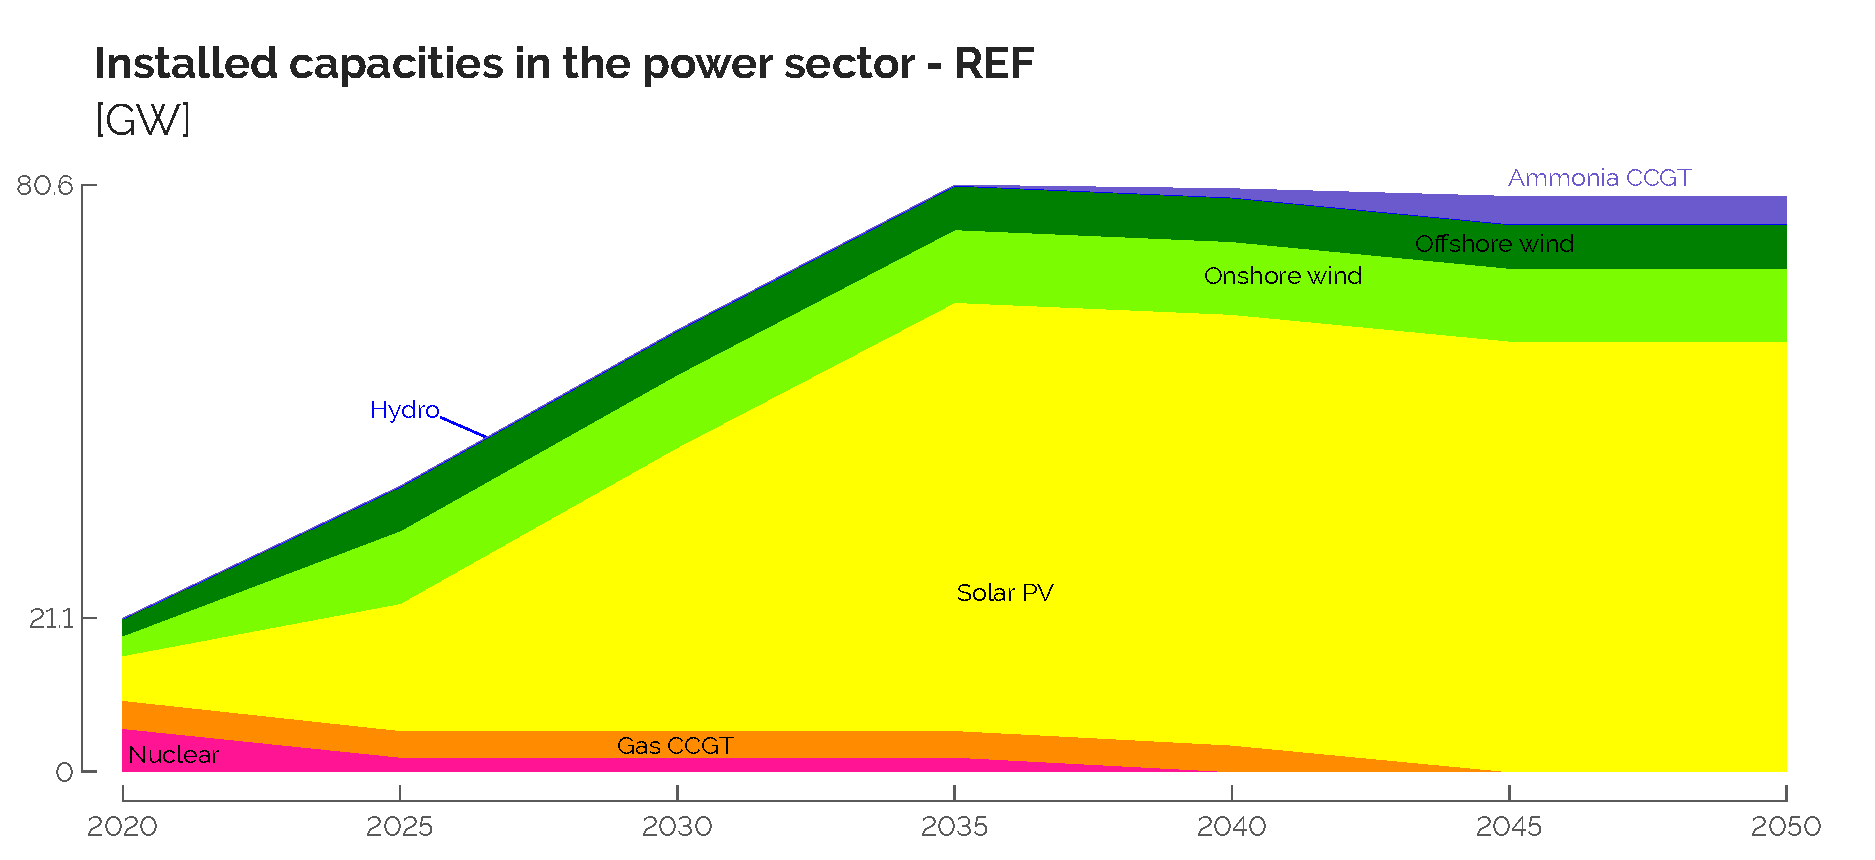
\includegraphics[width=\textwidth]{Elec_Tech_Cap_REF.pdf}
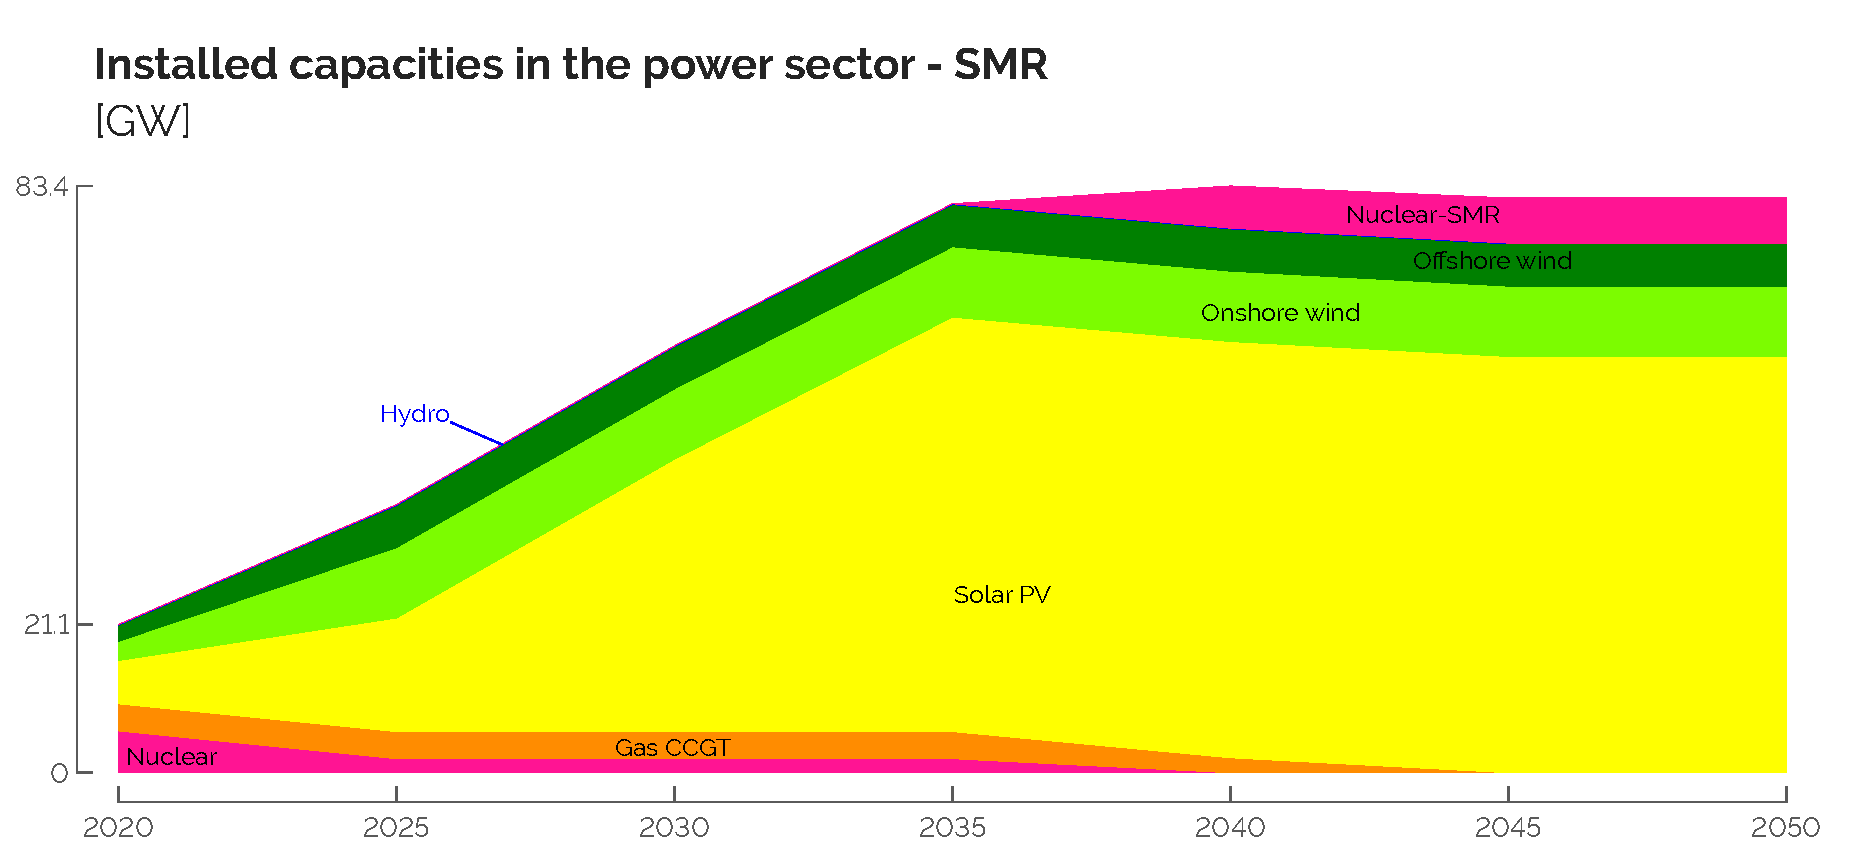
\includegraphics[width=\textwidth]{Elec_Tech_Cap_SMR.pdf}
\caption{Installed capacities in the power sector in the REF (top) and SMR (down) scenarios. As soon as available (\ie 2040), \acrfull{SMR} is deployed to its maximum potential (\ie 6\,GW) to substitute more expensive flexible generation units (\ie methane and ammonia \gls{CCGT}).}
\label{fig:results_deter_tech_cap_elec}
\end{figure}

When assessing the electricity production-versus-consumption-balance (\Cref{fig:results_deter_layer_elec}), \gls{SMR}, as a cheaper, flexible and low-emitting power generation system, produces to its full capacity. Given the 15\% maintenance off-time assumed in this work, this represents 44.6\,TWh by 2050. In comparison, in 2020, conventional nuclear power plants produced 34.4\,TWh in Belgium. This resurgence of nuclear electricity occurs at the expense of other, although more efficient, technologies: \gls{CCGT} and industrial \gls{CHP}. Besides the unchanged end-use-demand compared with the REF case, we observe a slight increase in the electrification of the rest of the system: +9.4\% which corresponds to +5.8\,TWh, mostly consumed by electric heaters in industry (+48\%) to produce industrial high-temperature heat.

\begin{figure}[t!]
\centering
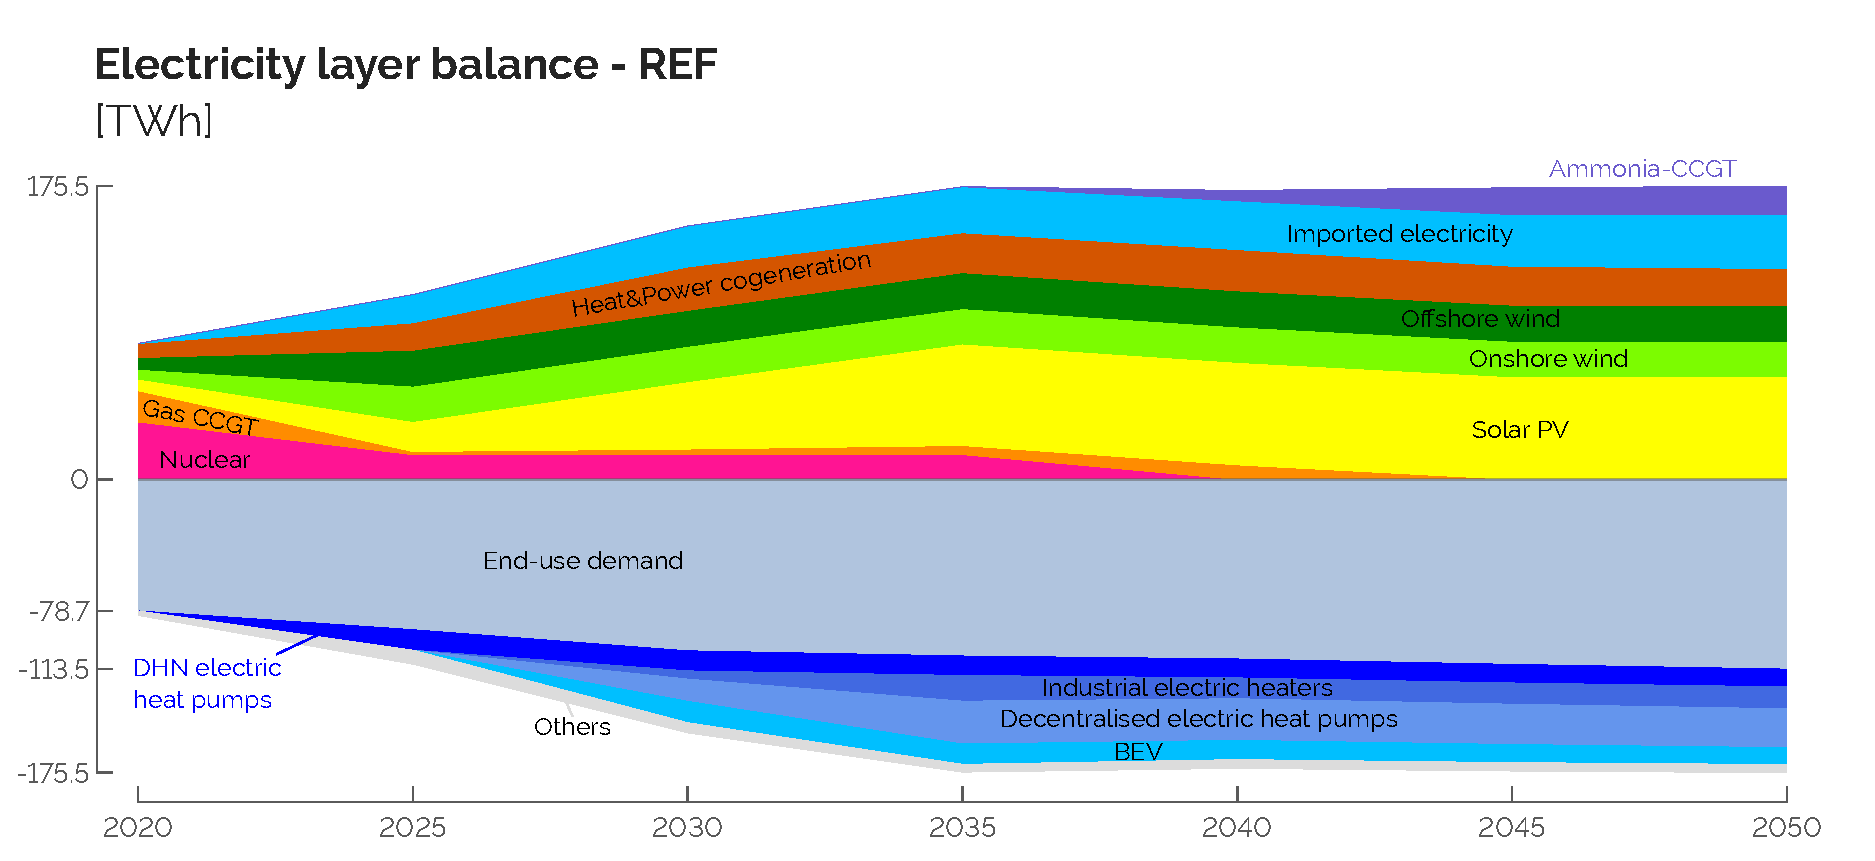
\includegraphics[width=\textwidth]{Elec_Layer_REF.pdf}
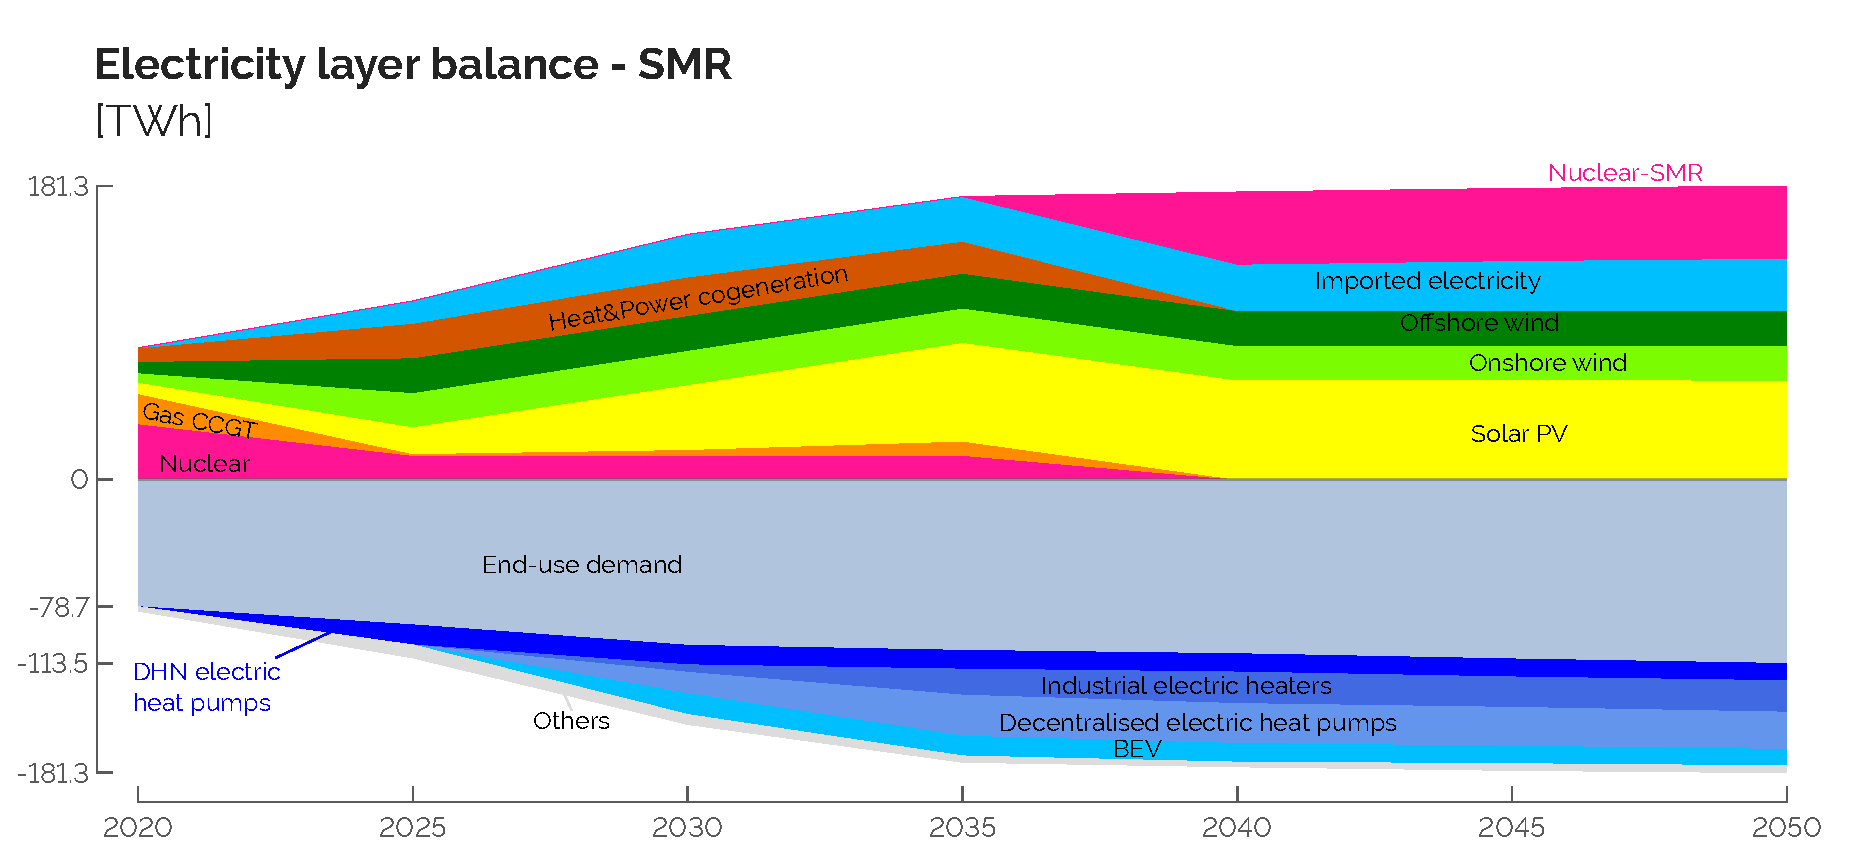
\includegraphics[width=\textwidth]{Elec_Layer_SMR.pdf}
\caption{Balance between the production and the consumption of electricity in the REF (top) and SMR (down) scenarios. The production of electricity from \gls{SMR} substitutes more efficient technologies (\ie \gls{CCGT} and \gls{CHP}) and boosts the electrification of the rest of the system, mostly the industrial high-temperature heat sector.}
\label{fig:results_deter_layer_elec}
\end{figure}

\newpage
\subsubsection{System-level impacts}
\label{subsubsec:atom_mol:results_deter_overall}
First of all, the 6\,GW \gls{SMR} installed from 2040 allow reaching a 3.3\% (-36.9\,b€) cheaper overall transition (\Cref{fig:results_deter_overall_emissions_sector}). Over the 30-year transition, this represents an annual cost saving equal to 0.2\% of the Belgian GDP. Thanks to the perfect foresight approach, the model knows ahead that cheaper and low-emitting \gls{SMR} will be available in the future. As the model can freely spend the constrained \ce{CO2} budget over the transition, cost-savings also occur before 2040. These early-stage cost-savings are equally shared between the extended use of cheaper \gls{LFO} to produce \gls{HVC} and the delayed deployment of \gls{PV}. Then, the capital-intensive investments in \gls{SMR}, mostly recovered by the end of the transition as salvage value, are widely compensated by the smaller resource-related OPEX. This leads, at the end, aggregating the OPEX and the annualised CAPEX, to a system that is yearly 4.4\,b€ (8.8\%) cheaper by 2050 than in the REF case (Figure \ref{fig:results_deter_overall_emissions_sector}).

\begin{figure}[htbp!]
\centering
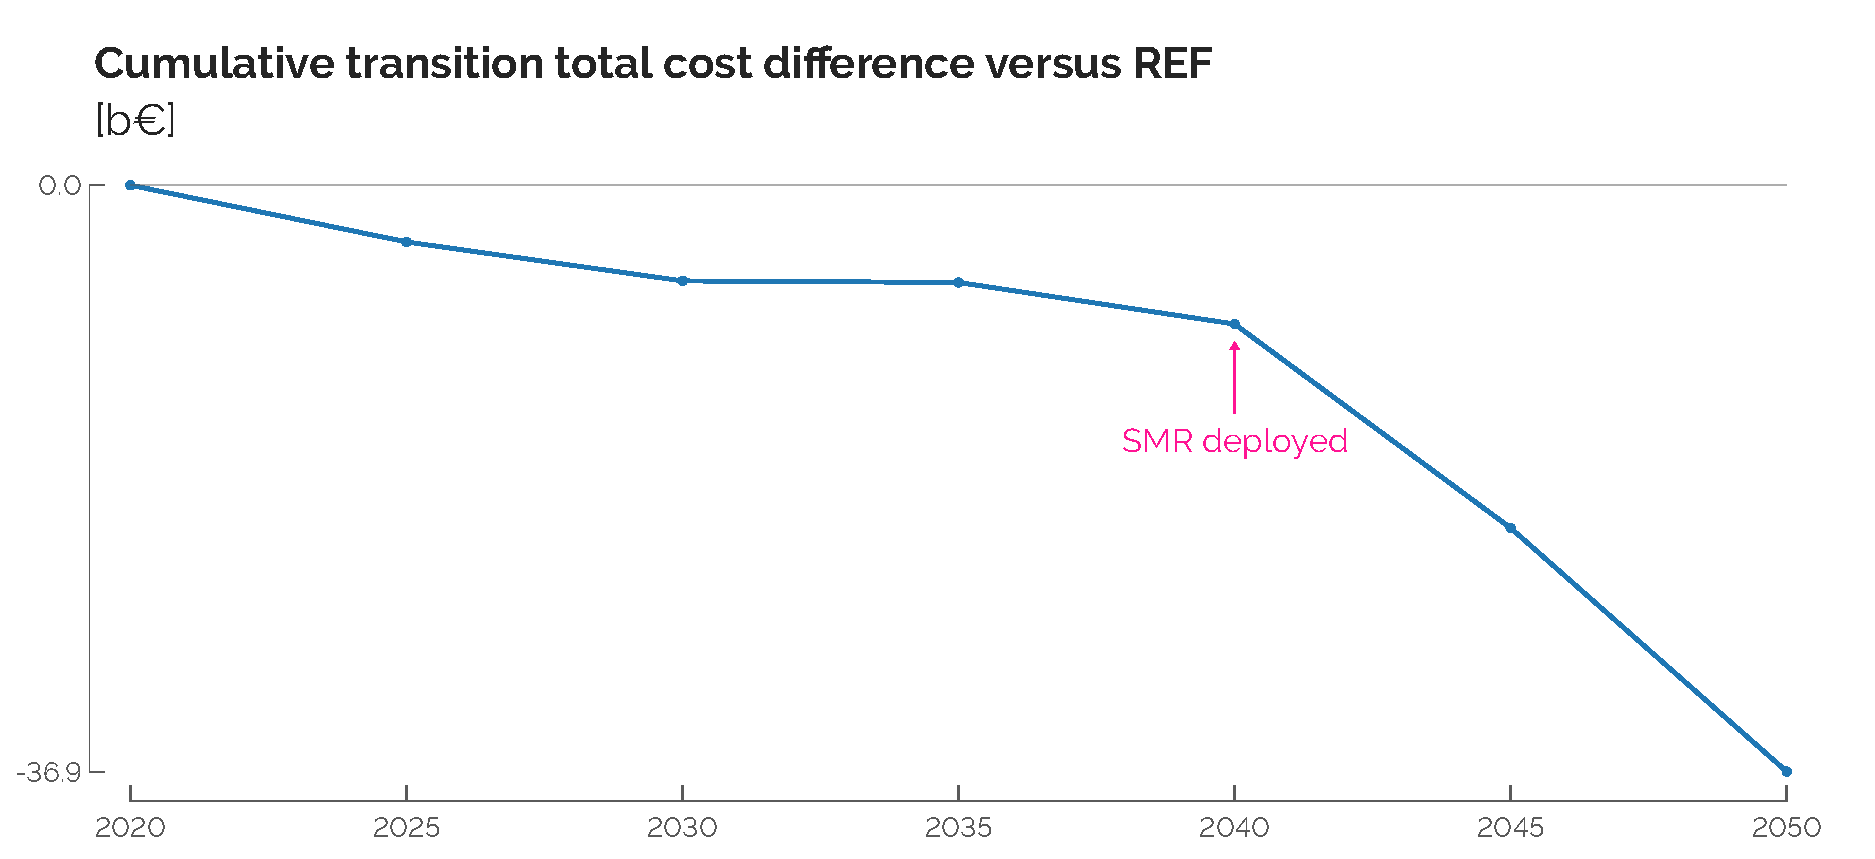
\includegraphics[width=\textwidth]{Cum_total_cost_diff_REF.pdf}
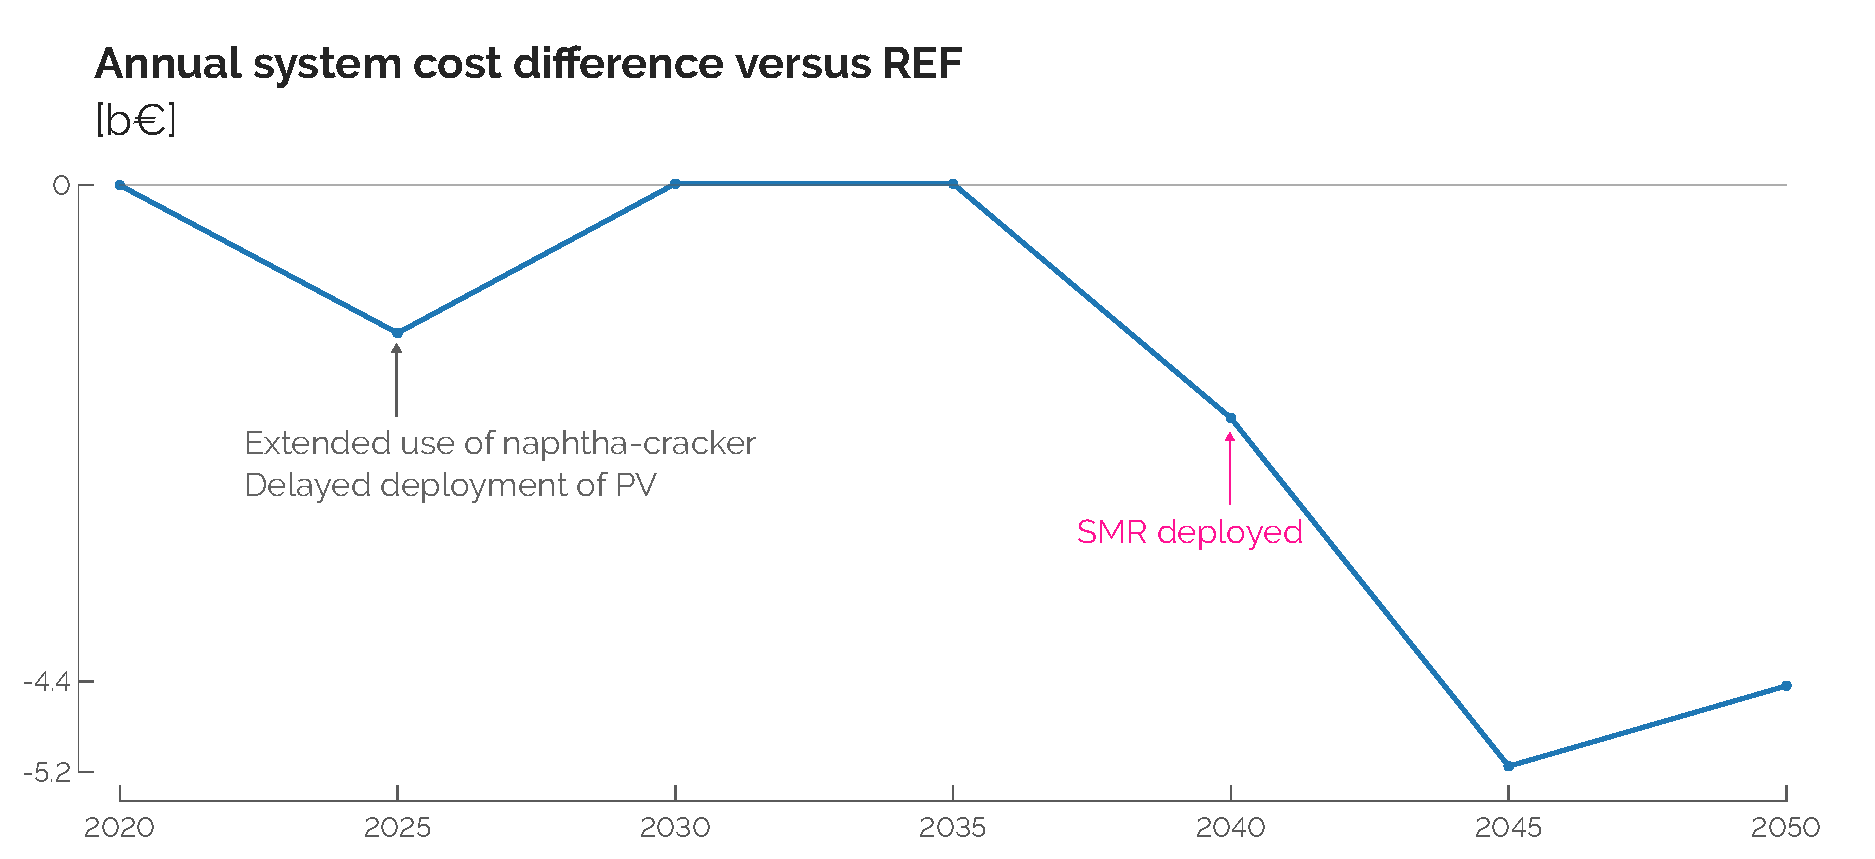
\includegraphics[width=\textwidth]{System_cost_DIFF.pdf}
\caption{(Top) Cumulative transition cost and (down) annual system cost differences between the SMR and the REF cases. Including \gls{SMR} ends up in a cheaper overall transition (-36.9\,b€) and cheaper whole-energy system by 2050 (-4.4\,b€).}
\label{fig:results_deter_overall_emissions_sector}
\end{figure}

Extending the use of naphtha-crackers and, to a lesser extent, postponing the deployment of PV, lead to higher \ce{CO2} emissions at the beginning of the transition that are then compensated by the deployment of \gls{SMR} (\Cref{fig:GWP_per_sector_diff}). 

\begin{figure}[htbp!]
\centering
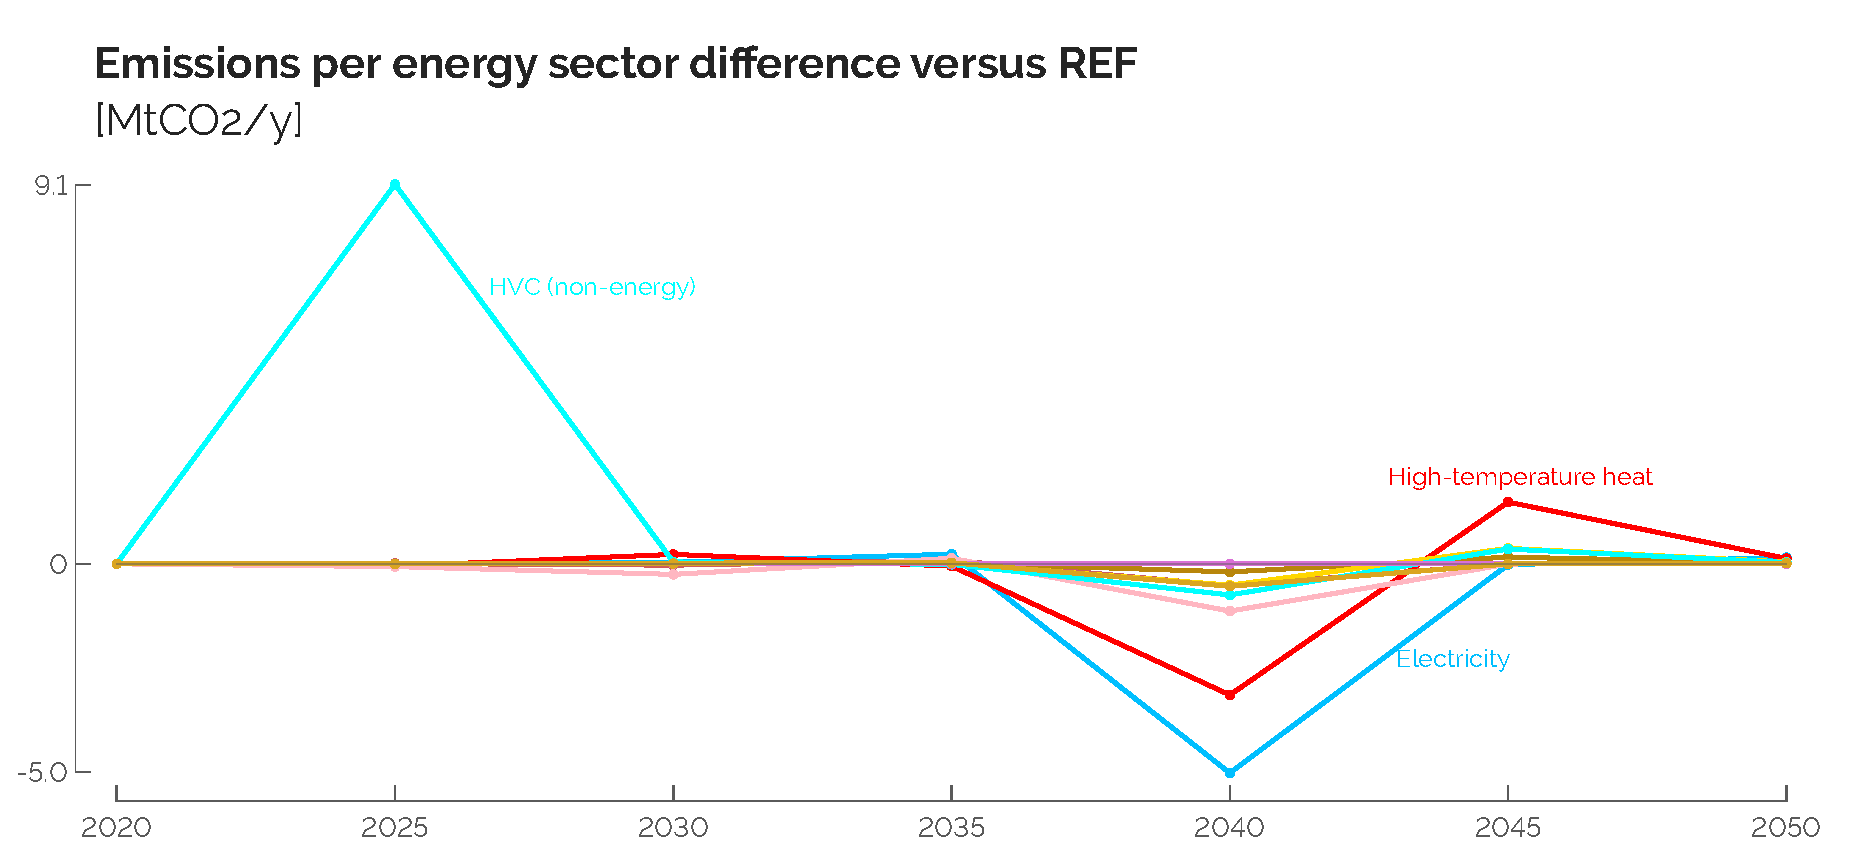
\includegraphics[width=\textwidth]{GWP_per_sector_diff.pdf}
\caption{Emissions per energy sector difference between the SMR and the REF cases. The deployment of \gls{SMR} from 2040 onward allows maintaining longer the use of \acrfull{LFO} for the production of \acrfull{HVC}.}
\label{fig:GWP_per_sector_diff}
\end{figure}

\newpage
Then, considering the primary energy mix shown in \Cref{fig:results_deter_energy_mix}, three phases in the transition can be identified. Before 2040, thanks to the perfect foresight approach, the model finds it more economical in 2025 to keep on using 33.2\,TWh of \gls{LFO} to produce \gls{HVC} through naphtha/LPG-cracking. In 2040, uranium-driven \gls{SMR} substitutes the electricity originally produced from industrial \gls{CHP} and \gls{CCGT} running respectively on fossil gas and renewable ammonia. Finally, from 2045 onward, the significant drop in the consumption of electrofuels comes from the same industrial \gls{CHP}. This is the illustration of the atom-molecules dilemma where the consumption of local renewables is, on its side, not much affected. In other words, \gls{SMR} competes with importing electrofuels while both support the integration of local solar and wind energies. Then, like the power sector, the SMR case ends up in a less efficient whole-energy system by 2050 at it consumes 47\,TWh (+12.7\%) primary energy more to supply an unchanged \gls{EUD}. Interestingly, in both cases, given the assumptions made on the \gls{GWP} of the resources (\ie $\mathit{gwp}_{\mathrm{op,electrofuels}}=0$\,kt$_{\ce{CO2},\text{eq}}$/GWh and $\mathit{gwp}_{\mathrm{op,uranium}}=0.004$\,kt$_{\ce{CO2},\text{eq}}$/GWh), the constraint on the \ce{CO2} budget leads to ``carbon neutrality'' by 2050\footnote{The model being constrained to keep on using all the waste that would keep on being locally produced, the system in 2050 reaches a $\sim 3.5\,Mt_{\ce{CO2},\text{eq}}$/year.}.

\begin{figure}[htbp!]
\centering
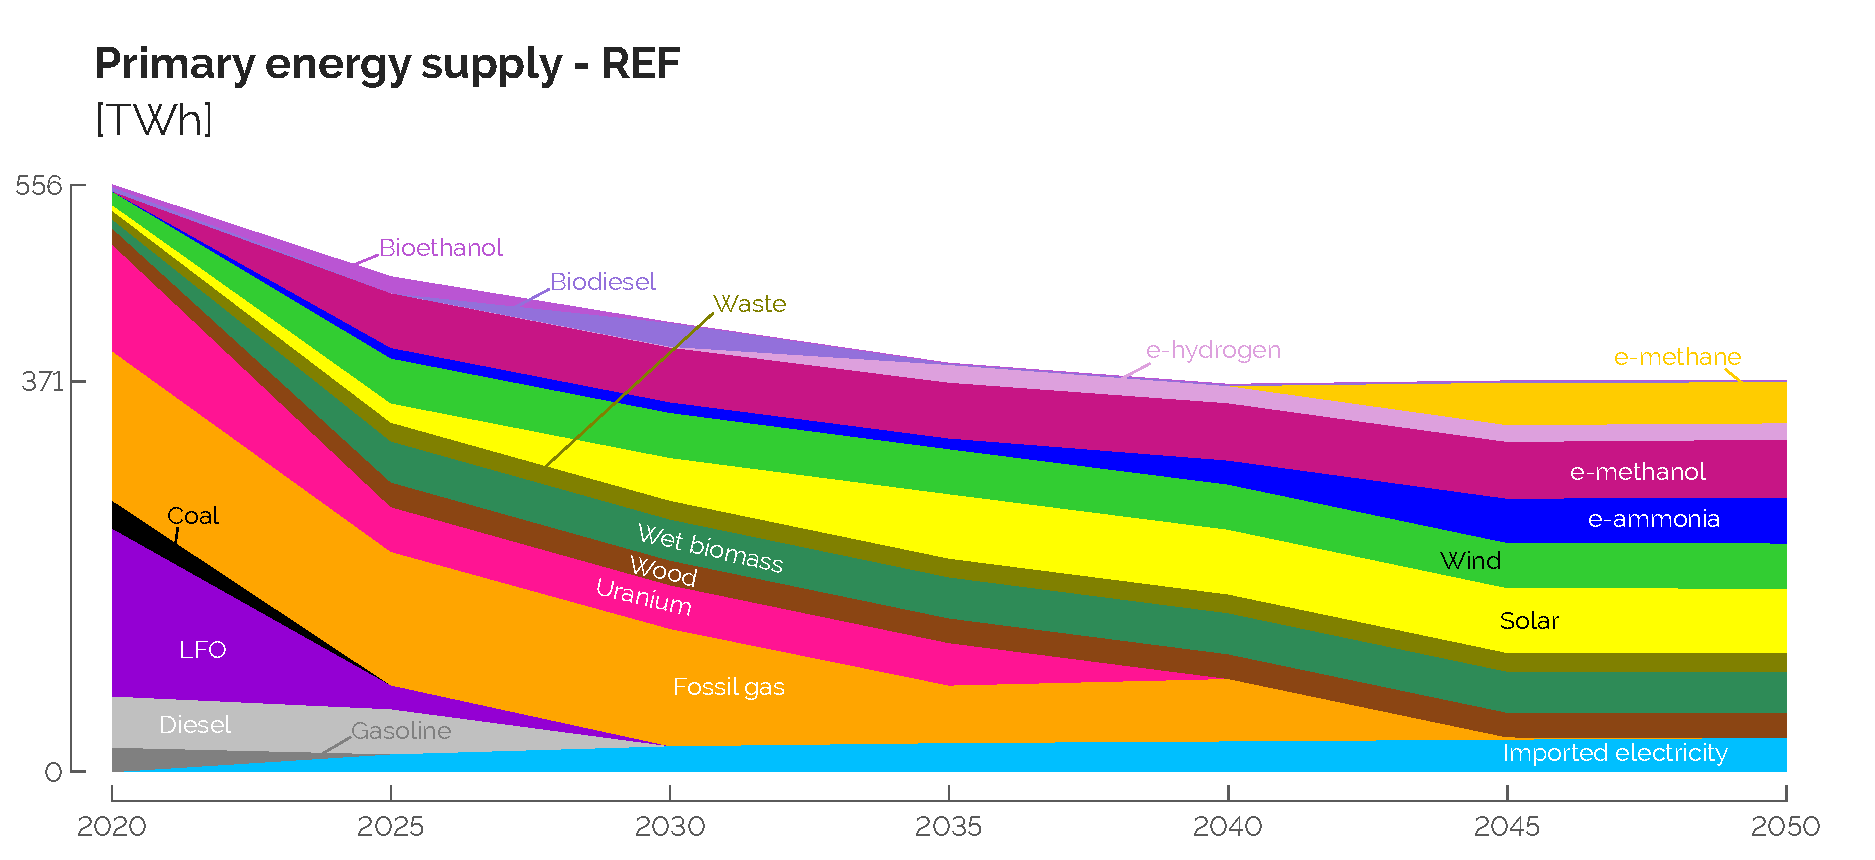
\includegraphics[width=0.8\textwidth]{Primary_mix_REF.pdf}
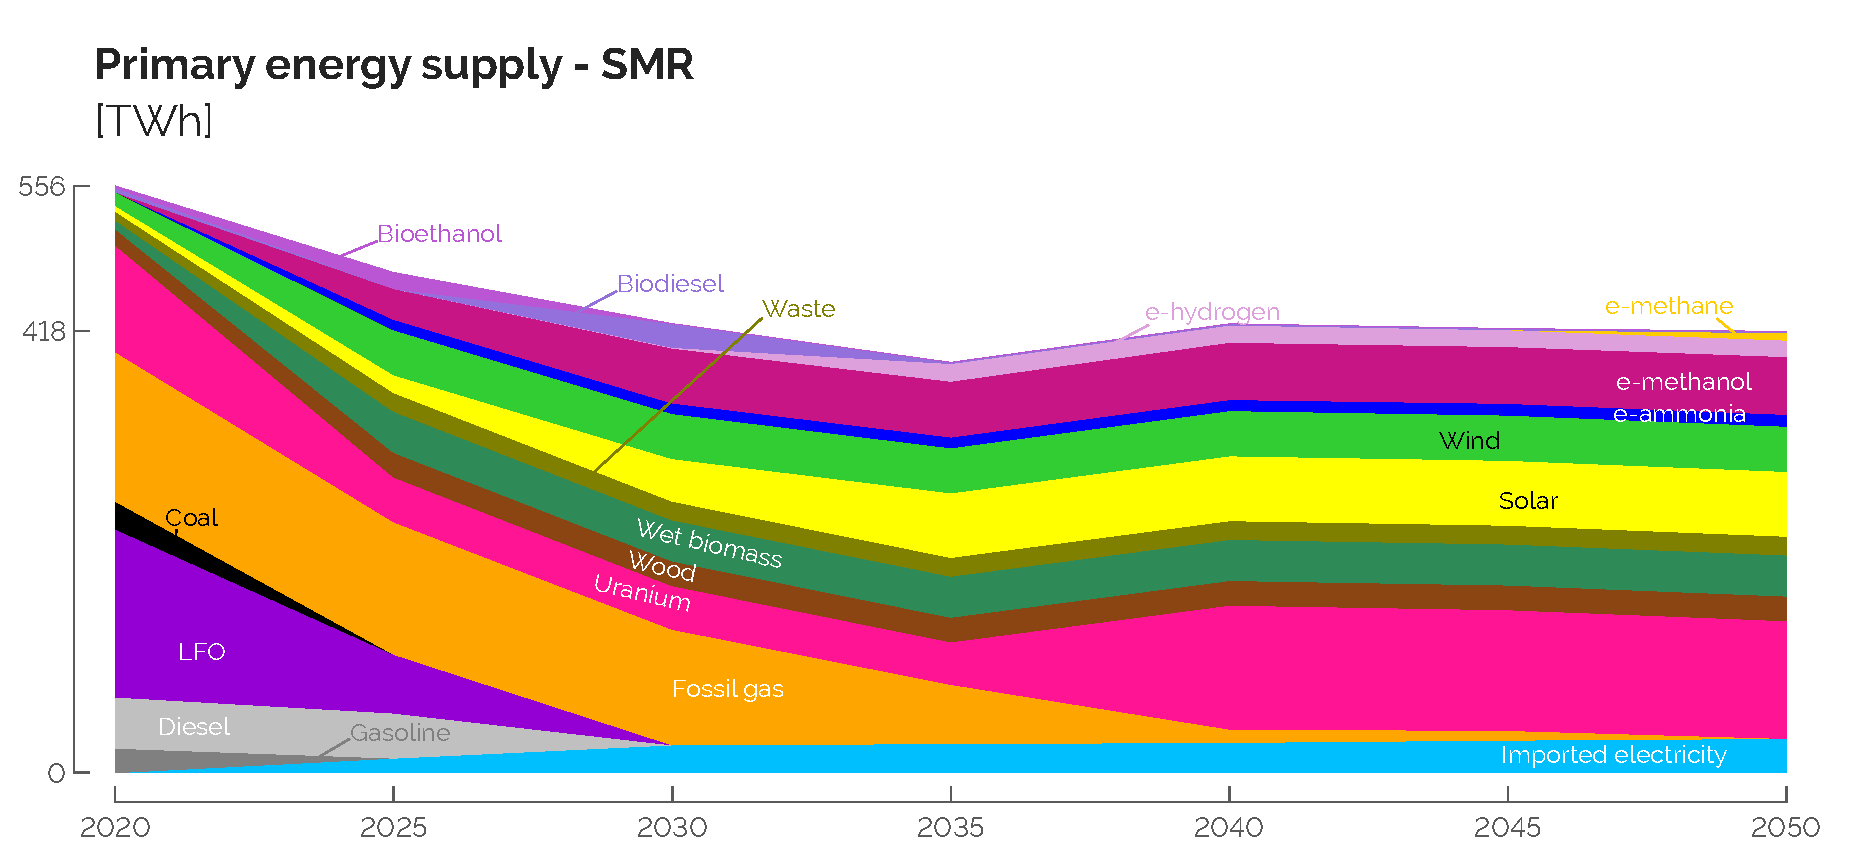
\includegraphics[width=0.8\textwidth]{Primary_mix_SMR.pdf}
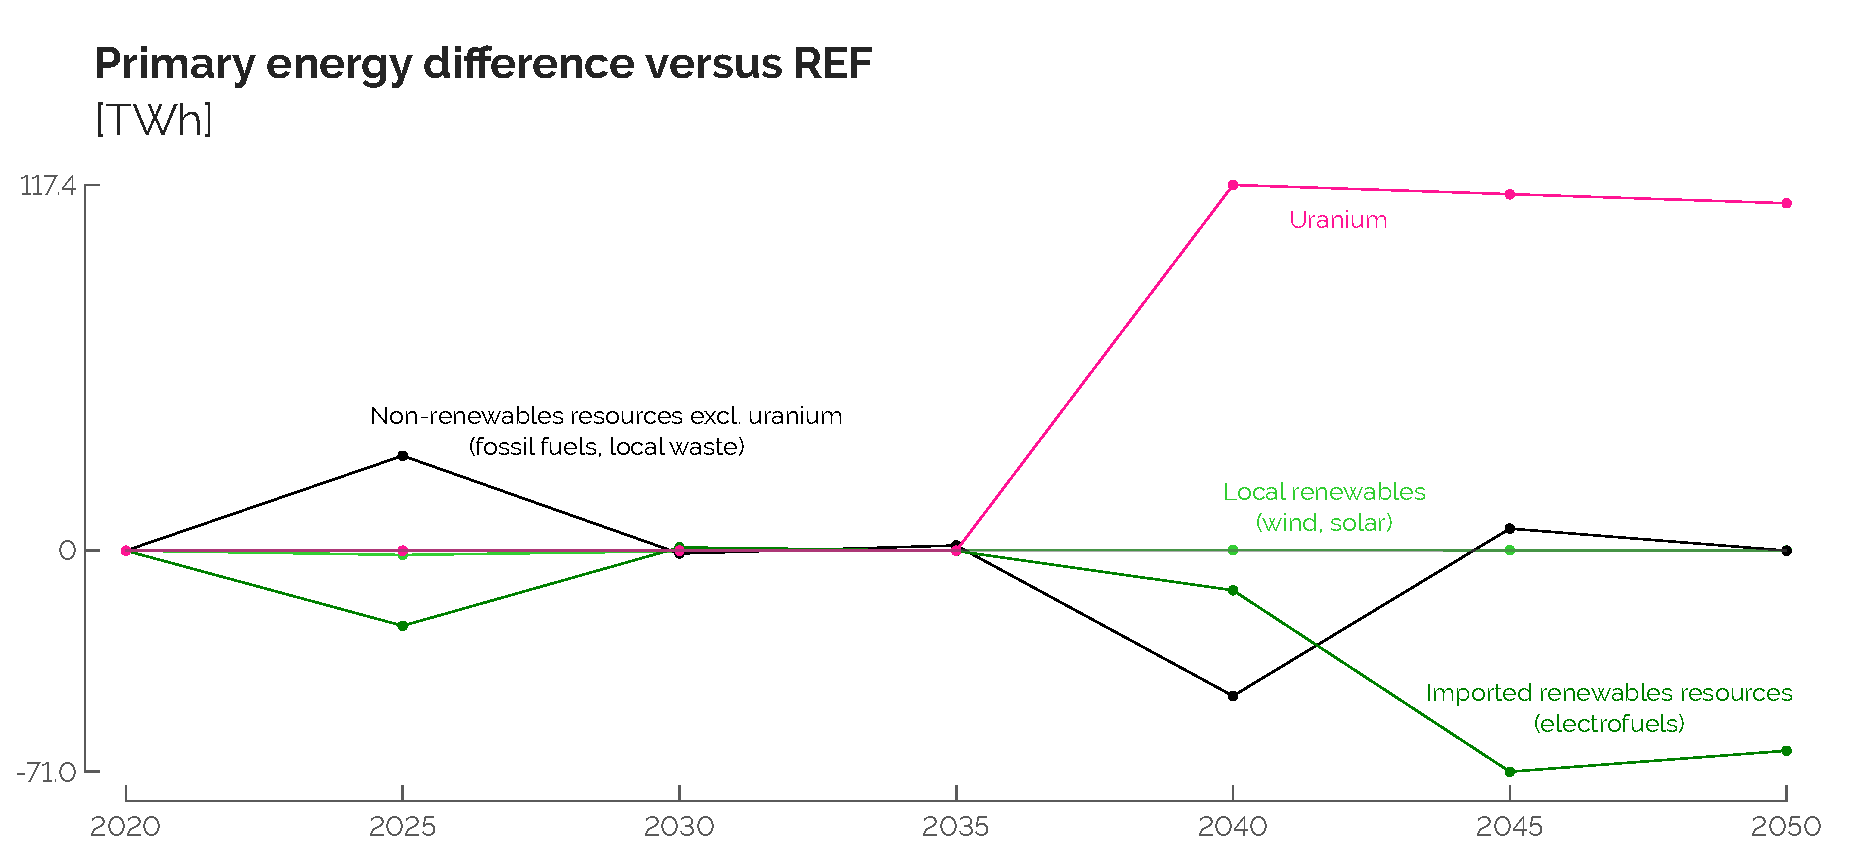
\includegraphics[width=0.8\textwidth]{Primary_mix_diff_uranium.pdf}
\caption{(Top) Primary energy mix over the transition for the REF and SMR cases. (Down) Difference of the mix between the two cases after aggregation per category. In line with \citet{rixhon2021terminology}, uranium is considered as a non-renewable resource. It is nevertheless dissociated from other non-renewable resources for the sake of clarity. The imported electricity is split between imported non-renewable and renewable resources between the current share of renewables, \ie 37.41\% \cite{eurostat_share_re_elec}, and an assumed 100\%-renewable European electricity mix by 2050.}
\label{fig:results_deter_energy_mix}
\end{figure}

\newpage
\subsubsection{Non-power sectors}
\label{subsubsec:atom_mol:results_deter_others}

Beyond the direct impact that \gls{SMR} has on the power sector, it also affects the other sectors. This is due to the sector-coupling typical of a whole-energy system optimisation \cite{contino2020whole}.\\

\myparagraph{High-temperature heat}\\

The main impact of including \gls{SMR} from 2040 onward on the high-temperature heat sector is (i) its higher direct electrification and (ii) the reduction of more efficient heat-and-power co-generation in the benefit of single-output industrial boilers. In the REF case, industrial electric heaters are mainly used to absorb the ``over-production'' of the 59\,GW solar-PV when fully deployed, on sunny days, and limit the yearly curtailment to a maximum of 0.3\,TWh, 0.5\% of the yearly 61\,TWh produced by solar-PV. With \gls{SMR}, by 2050, an additional 1.7\,GW (+13\%) of these heaters can rely on a more constant supply of defossilised electricity. This increases the load factor (31\%) and yearly production (48\%) of these industrial electric heaters. Then, given the 44.6\,TWh of electricity produced by \gls{SMR}, cogeneration units are less relevant and, by 2050, 2.6\,GW industrial gas boilers completely substitute \gls{CHP} to produce 16.6\,TWh (\ie 23\%) of the total production of high-temperature heat.\\

\myparagraph{Low-temperature heat}\\

This sector is marginally impacted. In both cases, the major shift of supply from decentralised to centralised productions operates early in the transition, to hit the constraint that \gls{DHN} cannot supply more than 37\% of the \gls{LT}-heat production. Then, from a mix of oil (53\%), gas (43\%) and wood (4\%) boilers for the decentralised production of \gls{LT}-heat in 2020, the system shifts towards electric \gls{HP} only by 2035. Similarly, for the centralised production of \gls{LT}-heat, electric \gls{HP} remains the most efficient and economical option.\\

\myparagraph{Mobility}\\

Passenger mobility is not affected either as the electrification of the system is preferentially done in this sector with \gls{BEV} substituting \gls{ICE} cars for the private sector by 2030. Regarding public mobility, trains and tramways supply their \textit{a priori} set maximum share, respectively, 50\% and 30\% complemented by \gls{CNG} buses substituting diesel-driven buses. Similarly, considering the freight transport, technology shifts (\ie from diesel to \gls{FC} trucks) or modal shares (\ie 53\%-47\% split between \gls{NG} and (bio)-diesel boats) are identical between the two cases.\\

\myparagraph{Non-energy demand}\\

The supply of ammonia (\ie from Haber-Bosch to direct import of renewable ammonia) and methanol (\ie import of renewable methanol) are unchanged between the two cases. However, as introduced previously, to produce \gls{HVC}, the full substitution of naphtha/LPG-cracking by \gls{MTO} is delayed as the emissions of the former are compensated by the later integration of \gls{SMR}.

\subsection{Uncertainty quantification on the cost, the atom and the molecules}
\label{subsec:atom_mol:results_uq}
Besides the detailed understanding of the deterministic results, it is important to challenge these conclusions accounting for the uncertainty of the parameters \cite{guevara2020machine}. After briefly assessing the \acrfull{GSA} on the total transition cost (Section \ref{subsubsec:atom_mol:results_uq_cost}), this section investigates more deeply the atom-molecules dilemma (Section \ref{subsubsec:atom_mol:results_atom_mol}). The Sobol' indices are computed for the import of renewable molecules and installed capacities of \gls{SMR}.

\subsubsection{Total transition cost}
\label{subsubsec:atom_mol:results_uq_cost}
Exhaustively listed in Appendix \ref{app:UQ_transition_cost}, \Cref{tab:UQ_short} gathers the most impacting parameters on the total transition cost. Per \citet{Turati2017}, parameters are considered as ``impacting'' if their Sobol' index is above the threshold $=1/d$, $d$ being the total number of uncertain parameters after the pre-selection phase. In this case, $d=34$, and, consequently, the threshold is equal to 2.9\%. \Cref{tab:UQ_short} shows that the cost of purchasing electrofuels is the most impacting parameter. On the contrary, the potentiality to install \gls{SMR} and its CAPEX have a much lower influence on the variation of the total transition cost. Given the uncertainty characterisation presented in Appendix \ref{subsec:cs:uncertainty}, there are 60\% chance that no \gls{SMR} could be installed. When $f_{\mathrm{max,SMR}}$ takes a value below 0.6, the variation of the total transition cost is only due to the variation of the other parameters. Then, in perspective with the scenario analysis of Section \ref{subsec:atom_mol:results_deter}, the 3.3\% reduction has been observed when \gls{SMR} is installed from 2040 onward. This represents only 10\% of the samples. Moreover, when it is possible, \gls{SMR} is always installed thanks to its characteristics: cheap and low-emitting fuel, a long lifetime leading to lower annualised CAPEX and higher salvage value. However, given its limited deployment, up to 6\,GW, \gls{SMR}-related parameters have a lower impact on the variation of the total transition cost. On the contrary, more expensive renewable electrofuels are always imported, to a smaller or larger extent depending on the sample. For instance, in the REF case, the imported electrofuels represent, by 2050, 152.9\,TWh (\ie 41\% of the primary energy mix) with an average 93€/MWh cost of purchasing and, over the entire transition, a 273\,b€ cumulative OPEX (\ie 25\% of the total transition cost).

\begin{table}[htbp!]
\caption{Total Sobol' indices of the uncertain parameters over the total transition cost. Where the cost of purchasing electrofuels is the top-1 parameter, \gls{SMR}-related parameters have a negligible impact on this cost.}
\label{tab:UQ_short}
\centering
\begin{tabular}{l c c}
\toprule
\textbf{Parameter}  & \textbf{Ranking} & \textbf{Sobol' index} \\	
\midrule
\textbf{Purchase electrofuels} & 1 & 46.8\% \\
Industry EUD & 2 & 23.2\% \\
Discount rate & 3 & 12.0\% \\
Purchase fossil fuels  & 4 & 5.7\% \\
$\vdots$ & $\vdots$ & $\vdots$\\
\textbf{Potential capacity \gls{SMR}} & 11 & 0.9\% \\
$\vdots$ & $\vdots$ & $\vdots$\\
\textbf{CAPEX \gls{SMR}} & 33 & $<$0.1\% \\
\bottomrule							

\end{tabular}
\end{table}

Given the relatively wide uncertainty range (\ie up to [-30.8\%; +24.0\%] by 2050) and, above all, the major share of the total demand, between 53\% and 60\%, the industrial \gls{EUD} is the second most impacting parameter. 

As the driving factor for the annualisation and the salvage value of the assets, the discount rate has a 12\% Sobol' index. As detailed in Appendix \ref{subsec:meth:ES_Pathway}, the model considers an overall discount rate for the entire system (\ie 1.5\% as a nominal value). In practice, the discount rate would vary depending on the technology investment risk. This variation would have, for instance, a major impact on the \gls{LCOE} of technologies like nuclear power plants \cite{world_nuclear_asso}, given the important capital needs and long time horizons \cite{IEA_Nuclear_2022}.

The cost of purchasing fossil fuels is also a key parameter in terms of variation of the total transition cost. However, due to the ambitious \ce{CO2} budget, phasing out of fossil fuels is urgent and makes their impact smaller than their renewable alternatives.

\Cref{fig:UQ_PDF_total_transition_cost} shows the distribution of the total transition cost given the 1260 samples. Stretching between 660\,b€ and 2050\,b€, the mean, the median and the nominal value (\ie REF case) are close to each other, respectively 1180\,b€, 1160\,b€ and 1080\,b€. Similarly to the analysis carried out by \citet{coppitters2023optimizing}, one observes here that the distribution is right-skewed. It could then be qualified as ``fragile'' as the top 50\% of the samples cover a bigger range (\ie between 1160 and 2050) than the bottom 50\% of the samples (\ie between 660 and 1160). In other words, the bad scenarios, resulting in a total transition cost higher than the median, have a bigger effect on this cost.

\begin{figure}[htbp!]
\centering
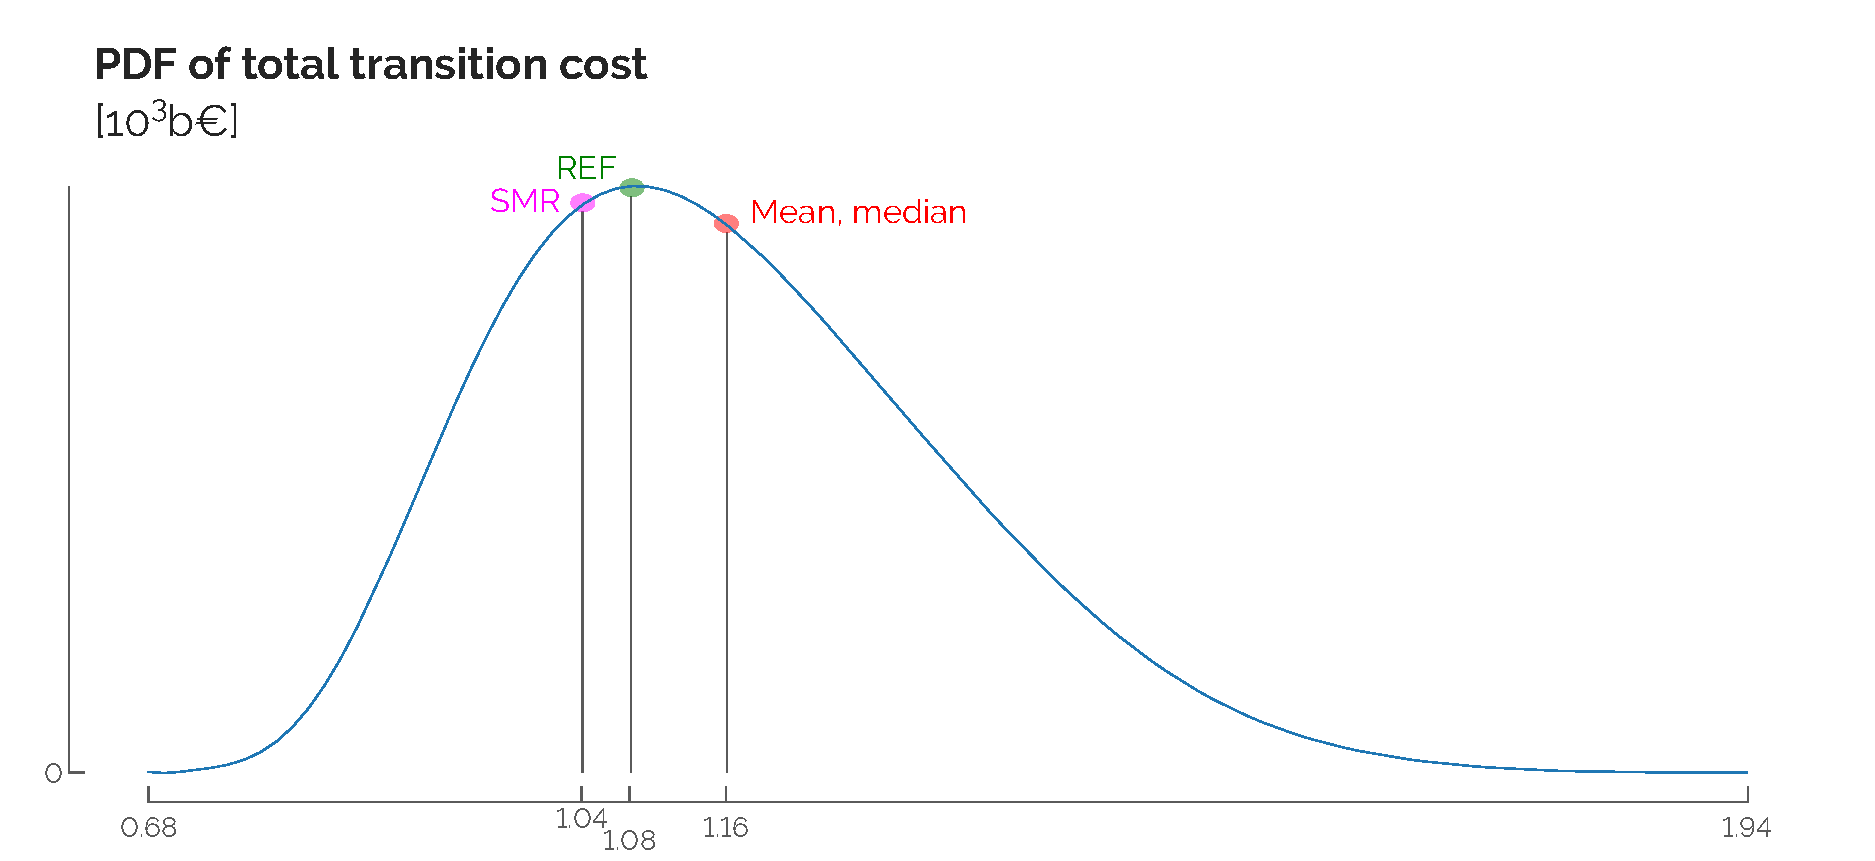
\includegraphics[width=0.8\textwidth]{UQ_PDF_total_transition_cost.pdf}
\caption{Distribution of the total transition cost over the 1260 runs of the \acrfull{GSA}. The mean, $\mu=1.18\cdot10^3$\,b€, is slightly higher than the median ($P_{50}=1.16\cdot10^3$\,b€) and the nominal cases cost, $1.08\cdot10^3$\,b€ and $1.04\cdot10^3$\,b€ respectively for the REF and SMR cases. Also, with a standard deviation, $\sigma=197$\,b€, a 95\%-confidence interval would be about [0.8; 1.6]$\cdot10^3$\,b€.}
\label{fig:UQ_PDF_total_transition_cost}
\end{figure}

\subsubsection{Atom and molecules}
\label{subsubsec:atom_mol:results_atom_mol}
The samples used to carry out the \gls{GSA} on the total transition cost, also provide the distribution of other outputs of the model like the import of renewable electrofuels over the transition. As the general trends are increasing, discrepancies exist between the different energy carriers (see \Cref{fig:results_uq_electrofuels}).
%
%\begin{figure}[htbp!]
%\centering
%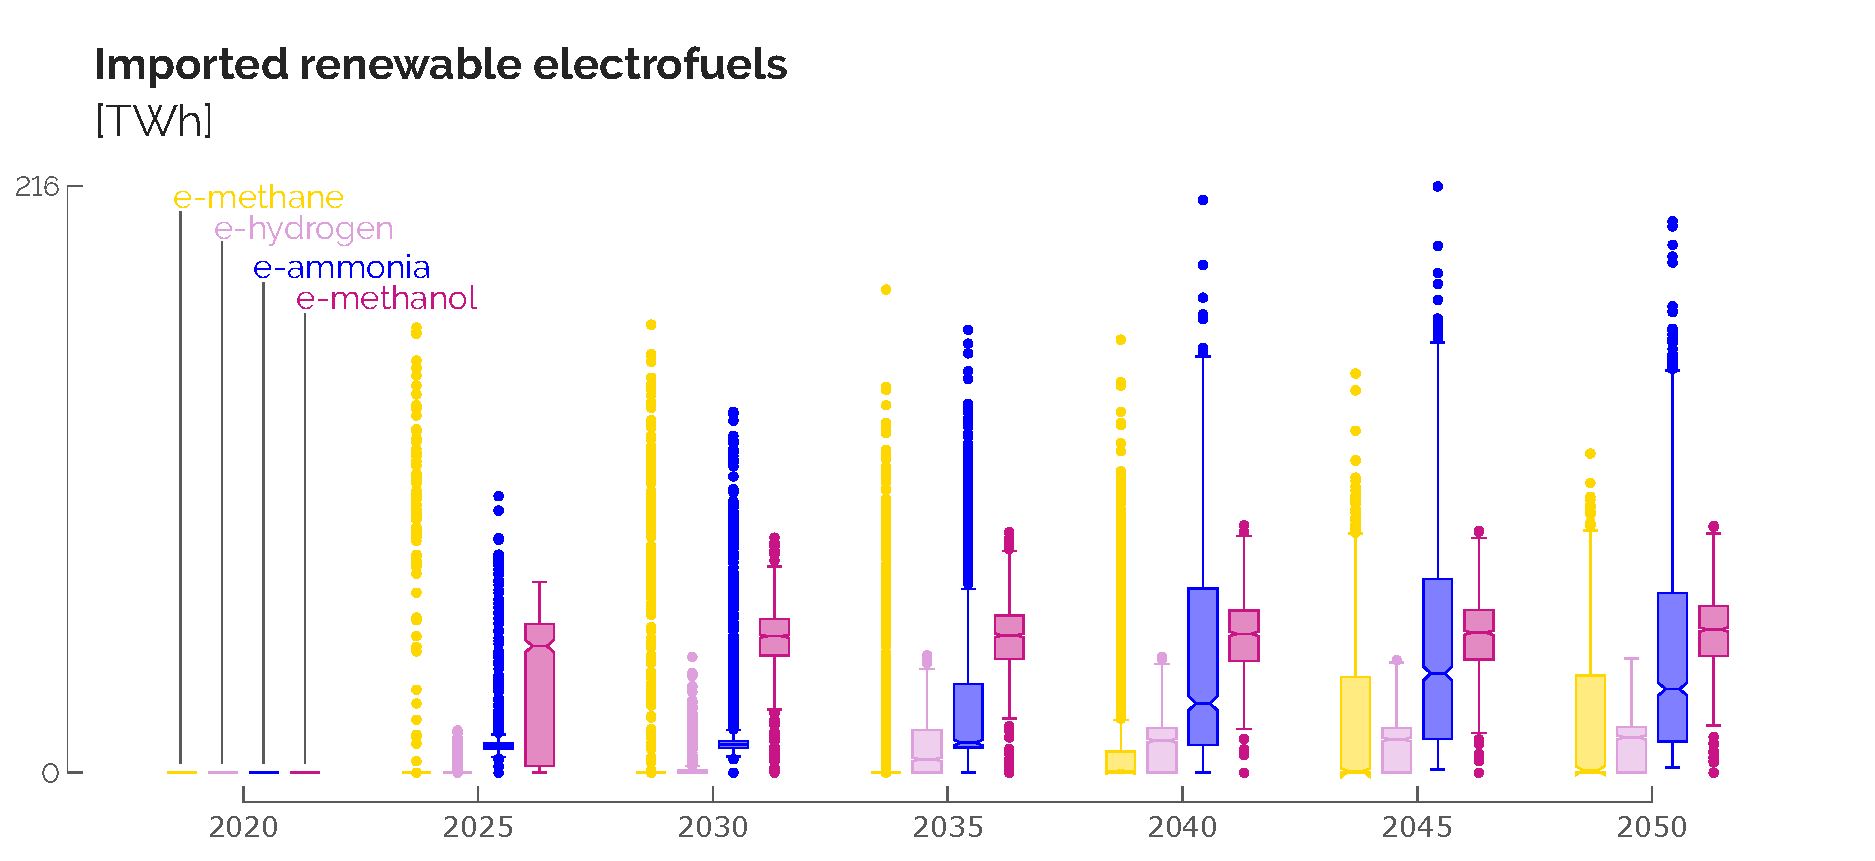
\includegraphics[width=0.7\textwidth]{UQ_Electrofuels.pdf}
%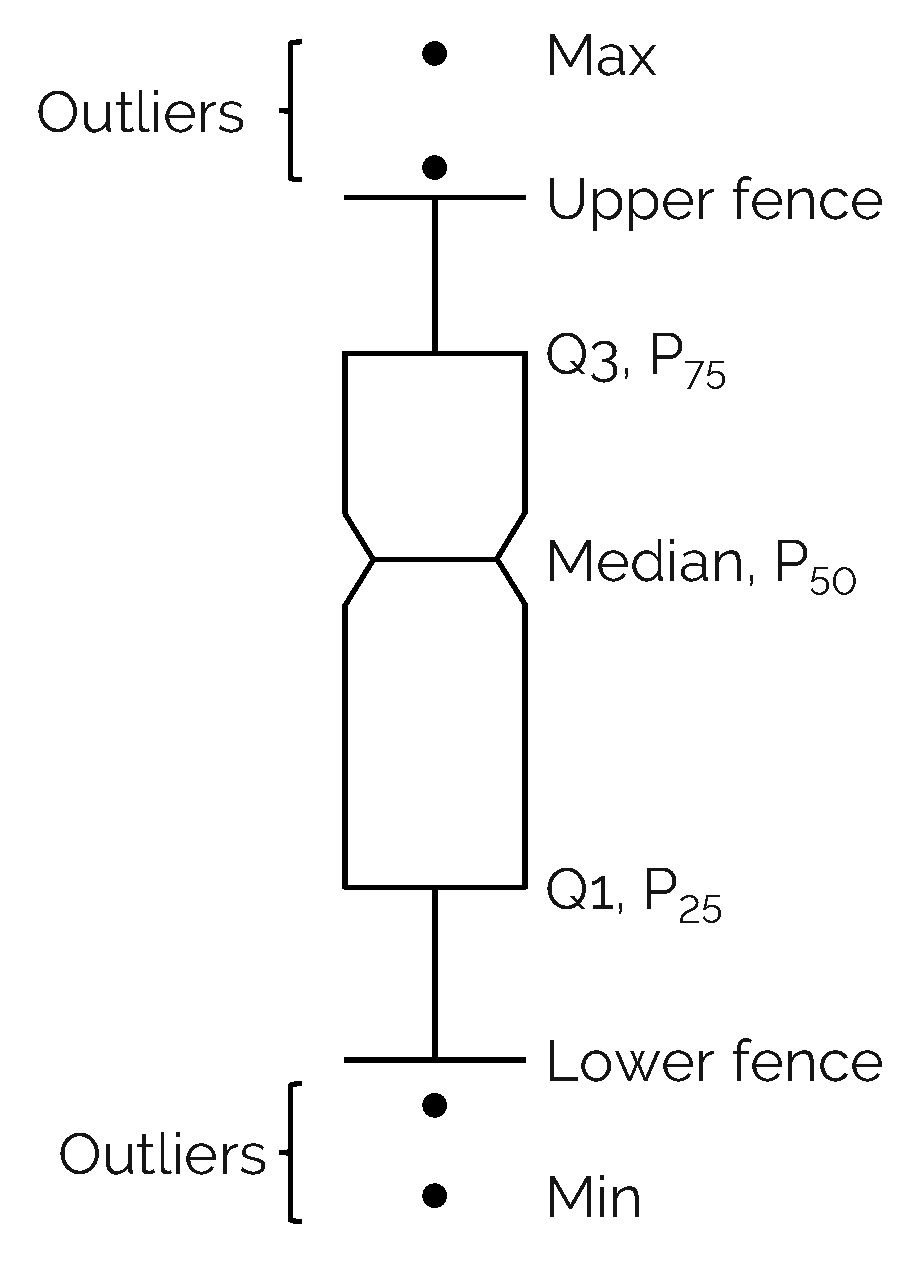
\includegraphics[height=4cm]{Schematic_boxplot.pdf}
%\caption{Distribution of the imported renewable electrofuels over the transition. Starting from no electrofuel in 2020, their respective import rises progressively along the transition (\ie increasing median) at different growth rates and with different ranges of values. Observations being either 1.5 times the interquartile range (IQR) less than the first quartile (Q1) or 1.5 times the interquartile range greater than the third quartile (Q3) are defined as outliers.}
%\label{fig:results_uq_electrofuels}
%\end{figure}

\begin{figure}[htbp!]
\centering
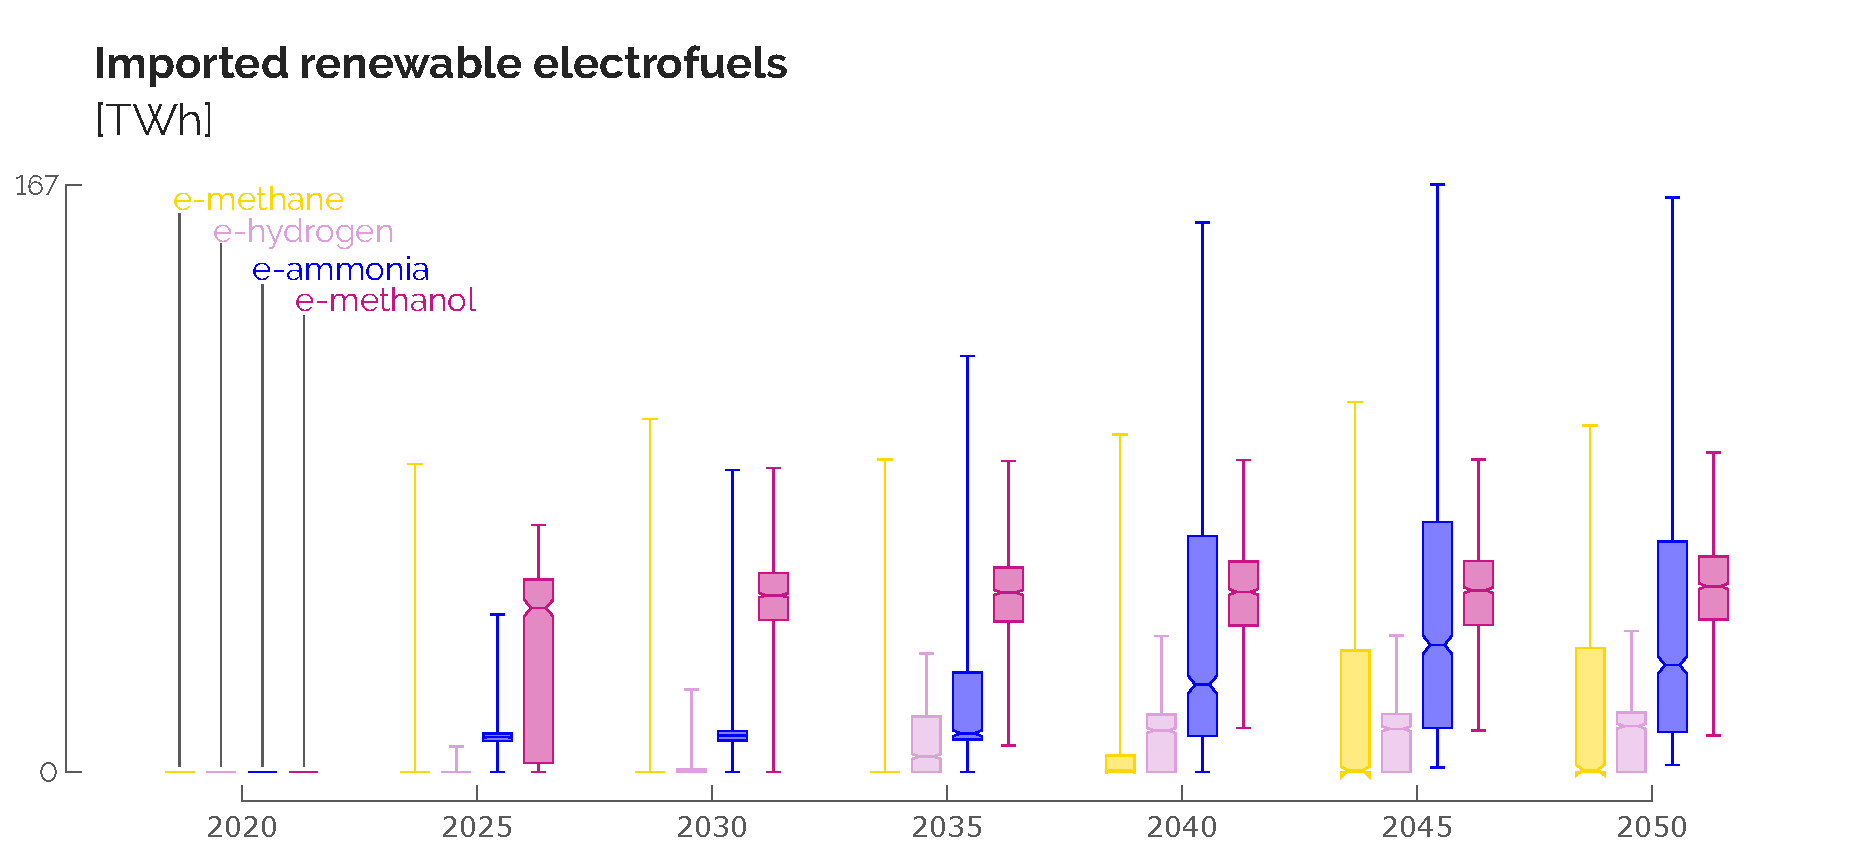
\includegraphics[width=0.7\textwidth]{UQ_Electrofuels_no_outlier.pdf}
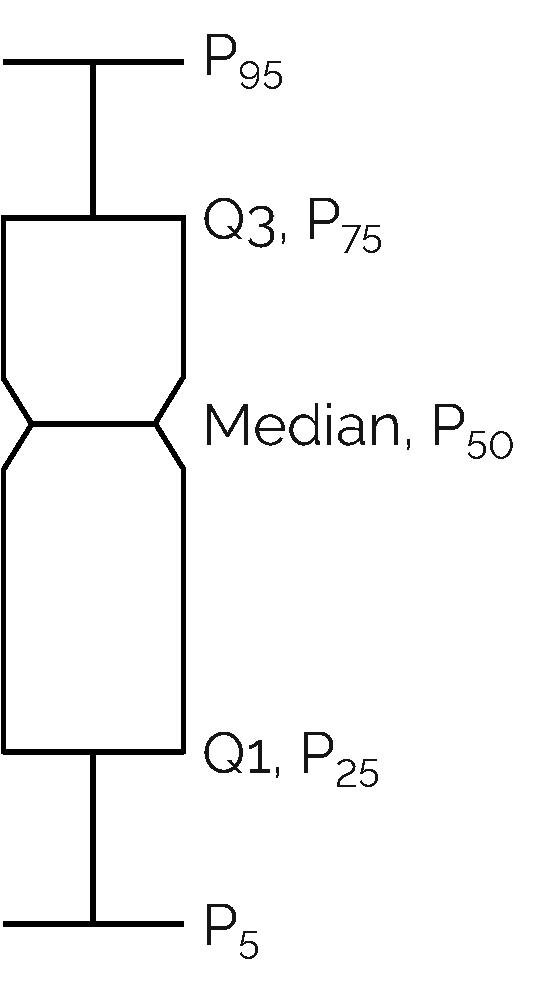
\includegraphics[height=3.8cm]{Schematic_boxplot_no_outlier.pdf}
\caption{Distribution of the imported renewable electrofuels over the transition. Starting from no electrofuel in 2020, their respective import rises progressively along the transition at different growth rates and with different ranges of values. }
\label{fig:results_uq_electrofuels}
\end{figure}

E-methane, as the renewable alternative to fossil methane, substitutes it, sometimes at a very early stage of the transition, 2025, and large extent, 163\,TWh, which is more than 6\% more than the total import of electrofuels in the REF case. The necessity to import this molecule is progressive through the transition to supply mostly industrial \gls{CHP} and boilers. 

E-hydrogen becomes rapidly the main stream of hydrogen in the system, reaching median and maximum values of 13.0\,TWh and 42.1\,TWh in 2050, respectively. Hydrogen is more frequently used in the mobility sector. Like in the REF case, fuel cell trucks are often the first option but, in some outlying cases, fuel cell cars and buses appear to completely substitute respectively \gls{BEV} cars and \gls{CNG} buses by 2050. Moreover, some samples lead to local production of methanol via the methanolation process, to produce up to 17.8\,TWh of methanol (\ie 33\% of the total supply of methanol of the nominal REF and SMR cases). 

Then, the imported e-ammonia rapidly becomes cost-competitive against its fossil alternative (see Appendix \ref{app:dem_res_tech}). At the early stage of the transition, e-ammonia substitutes fossil ammonia and the Haber-Bosch process. Where the initial purpose of ammonia is to satisfy a relatively limited \acrfull{NED} (\ie 10 $\pm$ 3\,TWh by 2050), the variation of its import is mostly due to the higher or lower need for ammonia-\gls{CCGT} as a flexible option to produce electricity. From 2035, out of the four considered electrofuels, the imported e-ammonia is the one exhibiting the largest uncertainty with, for instance, an interquartile range (IQR)\footnote{The interquartile range is the difference between the third quartile ($Q3$ or $P_{75}$) and the first ($Q1$ or $P_{25}$). It is an indicator of statistical dispersion around the median, $Q2$ or $P_{50}$.} of about 50\,TWh. In some extreme cases, e-ammonia is the most imported molecule, \ie up to 167\,TWh or 45\% of the total primary mix. 

Likewise, e-methanol early becomes the selected option to supply methanol even though alternatives like biomass-to-methanol are selected to supply, on average, 5\% of the demand for methanol. Its \gls{NED} represents, on average, 3\% of the total consumption of methanol. The variation of imported e-methanol is due to its role in the industrial production of \gls{HVC} through the \acrfull{MTO} process as it represents 95\% of the total consumption. For the remaining 2\%, methanol is also used to supply the freight transport sector via boats or trucks. More detailed statistics including the different sources of supply and consumption of gas, hydrogen, ammonia and methanol are provided in Appendix \ref{app:UQ_electrofuels}.\\

This part assesses the space of uncertainties, like \citet{pickering2022diversity} who investigated the space of feasibility to reach carbon neutrality in Europe. The trend lines of the key parameters can be drawn for these imports and the installed capacities of \gls{SMR} in 2050. We picked 2050 as it is the time of the transition where electrofuels, if imported, are imported in the largest amount compared to the other years of the transition. Next to the name of a parameter, one can read its Sobol' index versus the output of interest. For these outputs of interest, different from the total transition cost, the \gls{LOO} error is around 20\%. Even though this is higher than the threshold of \SI{1}{\%}, the Sobol' indices allow ranking the most impacting parameters (see Appendix \ref{subsec:meth:UQ}). Box plots also point out the distribution of this output for the extreme low or high values of some parameters.

For the import of e-methanol, industrial \gls{EUD} is, by far (\ie $\sim$80\% Sobol' index), the key factor (Figure \ref{fig:results_uq_samples_methanol}). Due to its own \gls{NED} but, above all, since it is the low-emitting alternative picked by the model to supply the significant \gls{NED} of \gls{HVC}, the lower this demand, the lower the need to import e-methanol, and vice versa. 

\begin{figure}[htbp!]
\centering
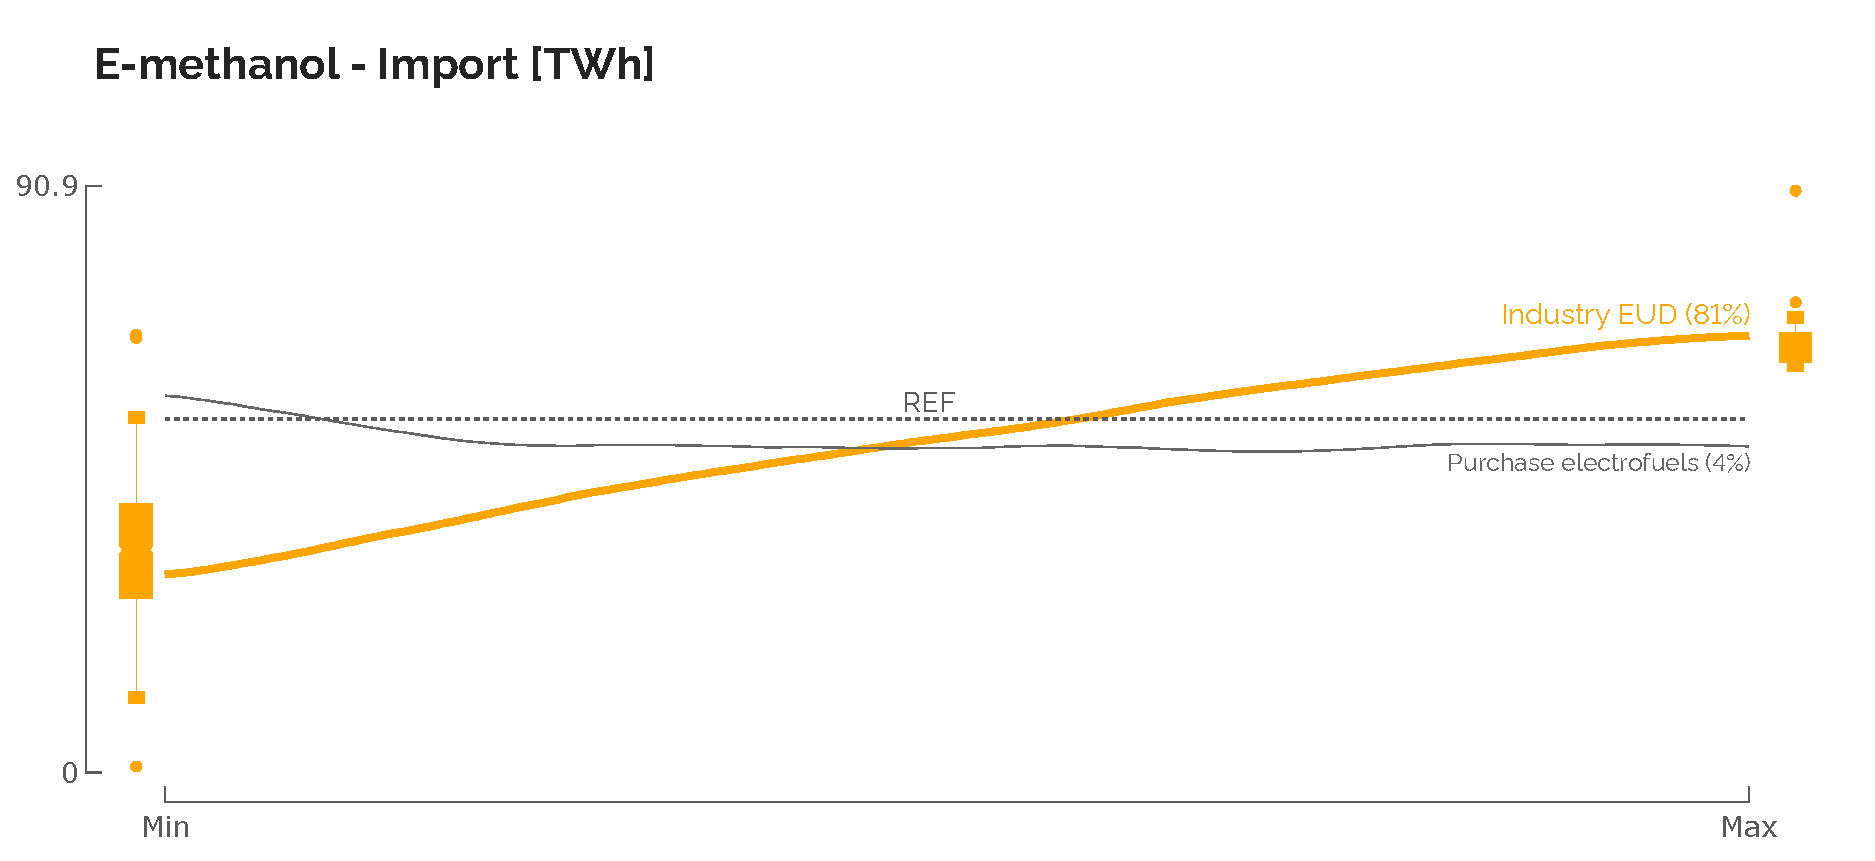
\includegraphics[width=0.8\textwidth]{UQ_Methanol_samples_2.pdf}
\caption{Trend lines of the key parameters (and their Sobol' index) on the import of e-methanol in 2050. Around these lines, box plots point out the distribution of the output of interest for the extreme values (either bottom-15\% or top-15\%) of some parameters. The grey dashed line gives the value of the output of interest in the REF case. }
\label{fig:results_uq_samples_methanol}
\end{figure}

About e-hydrogen, the sensitivity analysis highlights its dependence on various driving parameters, particularly those linked to the transport sector (Figure \ref{fig:results_uq_samples_H2}). The utilisation of e-hydrogen is most prevalent in \gls{FC} trucks, followed by \gls{FC} cars and buses to a lesser extent (Appendix \ref{app:UQ_electrofuels}). The adoption of fuel cell engines in trucks contributes, on average, to 63.5\% of the total road freight transport, thereby affecting the level of e-hydrogen imports. Consequently, the smaller the CAPEX of fuel cell engines, the more the system imports e-hydrogen. Similarly, the cost of purchasing electrofuels influences e-hydrogen imports. Subsequently, the cost of purchasing biofuels emerges as the third most influential parameter. Indeed, biodiesel trucks are the most picked alternative to \gls{FC} trucks to provide, on average, 27.6\% of the total. Additionally, \gls{CNG} buses are preferred in public road transport (34.9\%), followed by \gls{FC} buses (11.2\%) competing with biodiesel and hybrid biodiesel buses, accounting for 27.8\% and 26.1\%, respectively. Finally, the last noticeable parameter at stake is the CAPEX of electric vehicles. In competition with \gls{BEV} that stand for 83.4\% on average of the private mobility sector, the cheaper these cars are, the more cost-competitive are these vehicles, and vice versa, versus \gls{FC} cars (\ie 13.7\% of the total passenger mobility, on average).

\begin{figure}[htbp!]
\centering
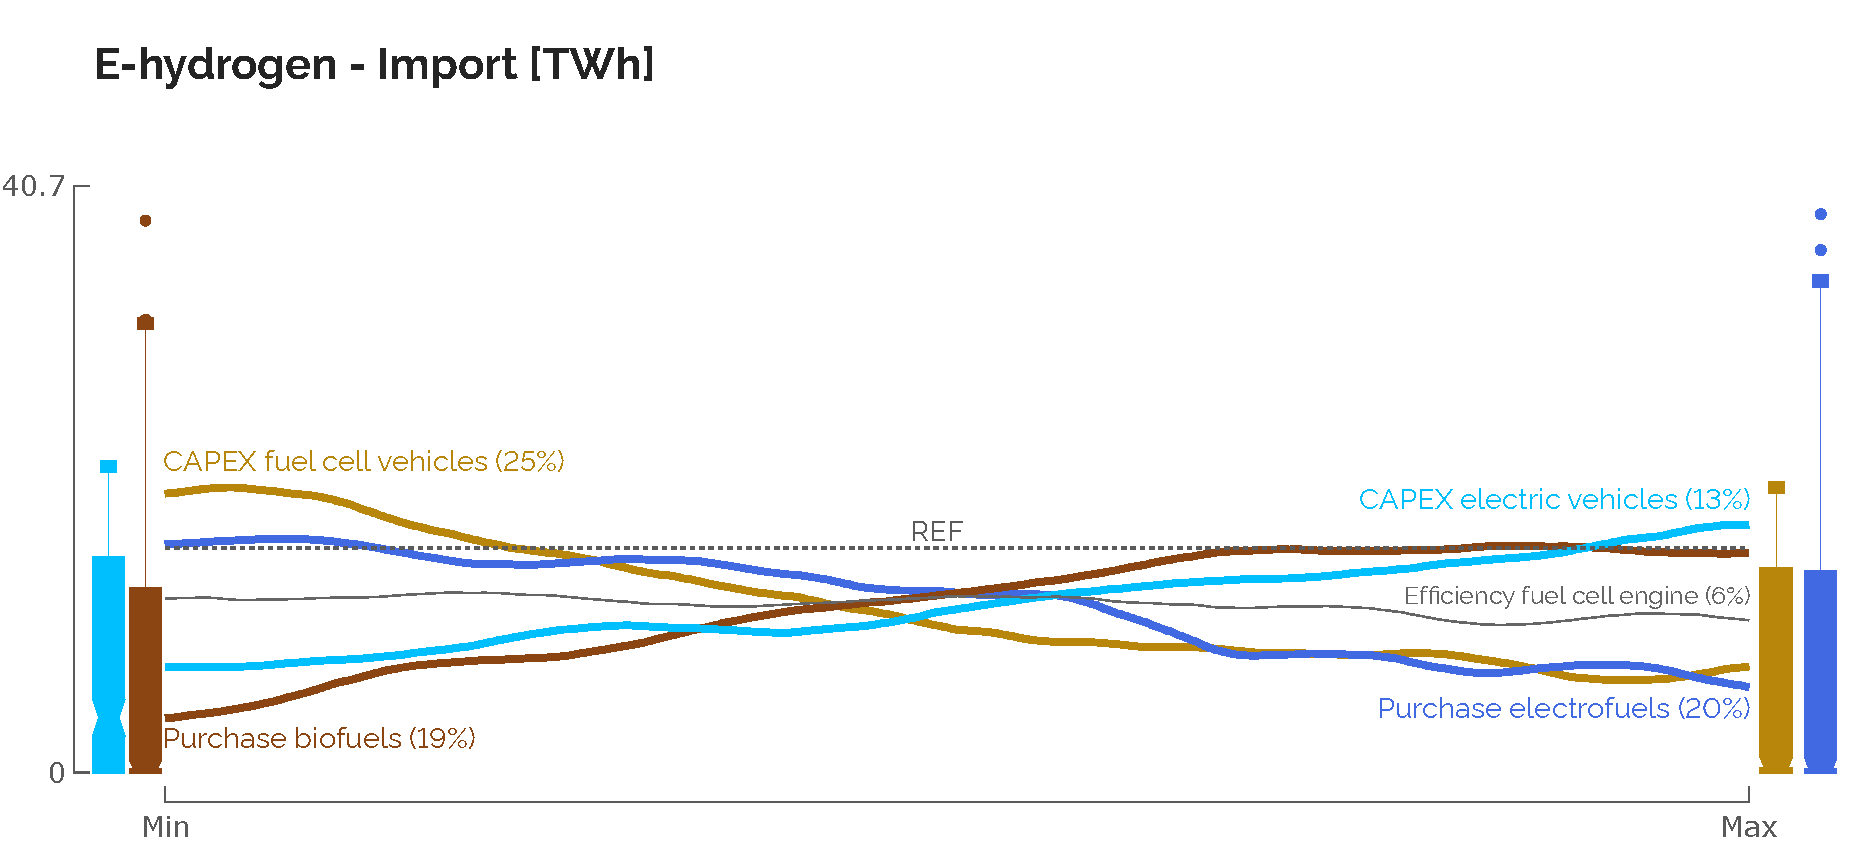
\includegraphics[width=0.8\textwidth]{UQ_H2_samples_2.pdf}
\caption{Trend lines of the key parameters (and their Sobol' index) on the import of e-hydrogen in 2050. Around these lines, box plots point out the distribution of the output of interest for the extreme values (either bottom-15\% or top-15\%) of some parameters. The grey dashed line gives the value of the output of interest in the REF case. }
\label{fig:results_uq_samples_H2}
\end{figure}

As already pointed out in Section \ref{subsubsec:atom_mol:results_deter_power_sector}, the installation of \gls{SMR} drastically reduces the import of e-ammonia (Figure \ref{fig:results_uq_samples_ammonia}). As ammonia \gls{CCGT} is the biggest consumer of ammonia by the end of the transition, low-emitting and cheaper electricity produced by \gls{SMR} (40 versus 151 €/MWh$_{\text{elec}}$) substitutes these \gls{CCGT}. With a higher cost of purchasing electrofuels, this import of e-ammonia drops down to 2.0\,TWh, 95.4\% less than in the REF case. Then, with a 12\%-Sobol' index, the cost of purchasing electricity from abroad, considered as renewable by 2050 and, therefore, a direct competitor to e-ammonia \gls{CCGT}, also affects the need of this molecule, especially when this cost is low.

\begin{figure}[htbp!]
\centering
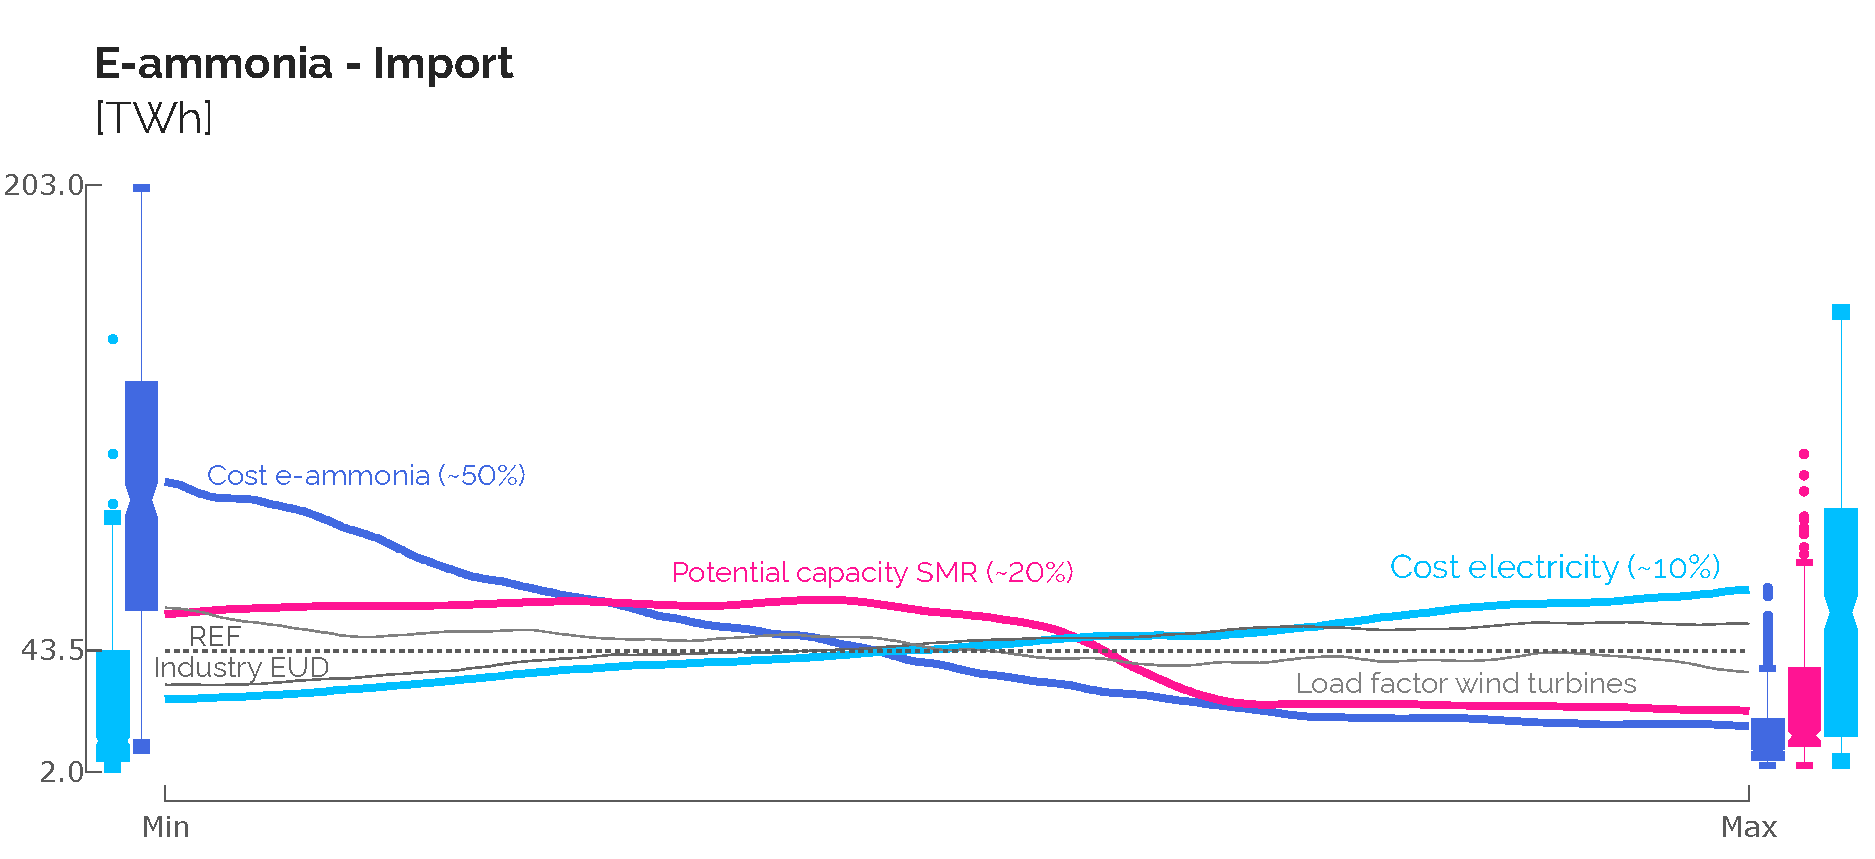
\includegraphics[width=0.8\textwidth]{UQ_Ammonia_samples_2.pdf}
\caption{Trend lines of the key parameters (and their Sobol' index) on the import of e-ammonia in 2050. Around these lines, box plots point out the distribution of the output of interest for the extreme values (either bottom-15\% or top-15\%) of some parameters. The grey dashed line gives the value of the output of interest in the REF case. }
\label{fig:results_uq_samples_ammonia}
\end{figure}

\newpage
As aforementioned, the industrial \gls{EUD} impacts the most the import of e-methane (Figure \ref{fig:results_uq_samples_gas}). This parameter directly dictates the demand of industrial high-temperature heat for which industrial gas \gls{CHP}, and industrial gas boilers to a lower extent, represent, on average over all the samples, respectively 25.6\% and 6.1\% of the total production. Then, considering the smaller-impact parameters, we notice that \gls{SMR} plays a non-negligible role. Indeed, if deployed, \gls{SMR} produces abundant low-emitting electricity for industrial electric heaters that substitute, even completely in some cases, gas alternatives. This confirms the observation made in Section \ref{subsubsec:atom_mol:results_deter_others}. Highly available local biomass also leads to smaller imports of e-methane to supply bio-hydrolysis and produce methane-equivalent gas. Finally, and surprisingly, the costs of purchasing electrofuels and fossil fuels have a positive and negative correlation with the amount of e-methane, respectively. In other words, by 2050, more expensive electrofuels result in more e-methane imports. On the contrary, cheaper electrofuels result in higher imports of fossil methane. Given the techno-economic optimum sought by EnergyScope, if electrofuels are more expensive, the system will, overall, import less of them, especially e-ammonia, mainly used by \gls{CCGT}. Subject to the \ce{CO2} budget for the transition, the system goes towards more efficient technologies, like industrial methane-\gls{CHP} to substitute e-ammonia-\gls{CCGT} in the production of electricity. First running on fossil gas, these \gls{CHP} consume more e-methane by 2050. On the contrary, if electrofuels are cheaper, there is more import of them, especially of e-ammonia. This leaves room for more emitting and cheaper resources to be used while respecting the \ce{CO2} budget, \ie coal in industrial boilers that produce, in these cases, on average 24\% of the high-temperature (HT) heat in 2050. In these cases, the use of coal in 2050 highlights that, with a sharper decrease of the emissions at early stages in the transition, the model finds a solution including highly-emitting resources (\eg coal) while respecting the \ce{CO2} budget. Consequently, there are smaller investments in methane \gls{CHP}, and consequently import of e-methane as more abundant renewable electricity is produced via e-ammonia-\gls{CCGT} and more HT-heat is supplied by industrial coal boilers. Even though we might expect that no more coal will be consumed in Belgium by 2050, the model still has the opportunity to use it if the \ce{CO2} budget allows it. Regarding the cost of purchasing fossil fuels, the parameter has mainly an impact on the import of fossil \gls{NG} as the most versatile energy carrier in the whole-energy system. If \gls{NG} is more expensive, the system will import less of it. Subsequently, the investments in methane-\gls{CHP} and boilers are more limited. This ends up in a smaller need for e-methane by 2050.

\begin{figure}[htbp!]
\centering
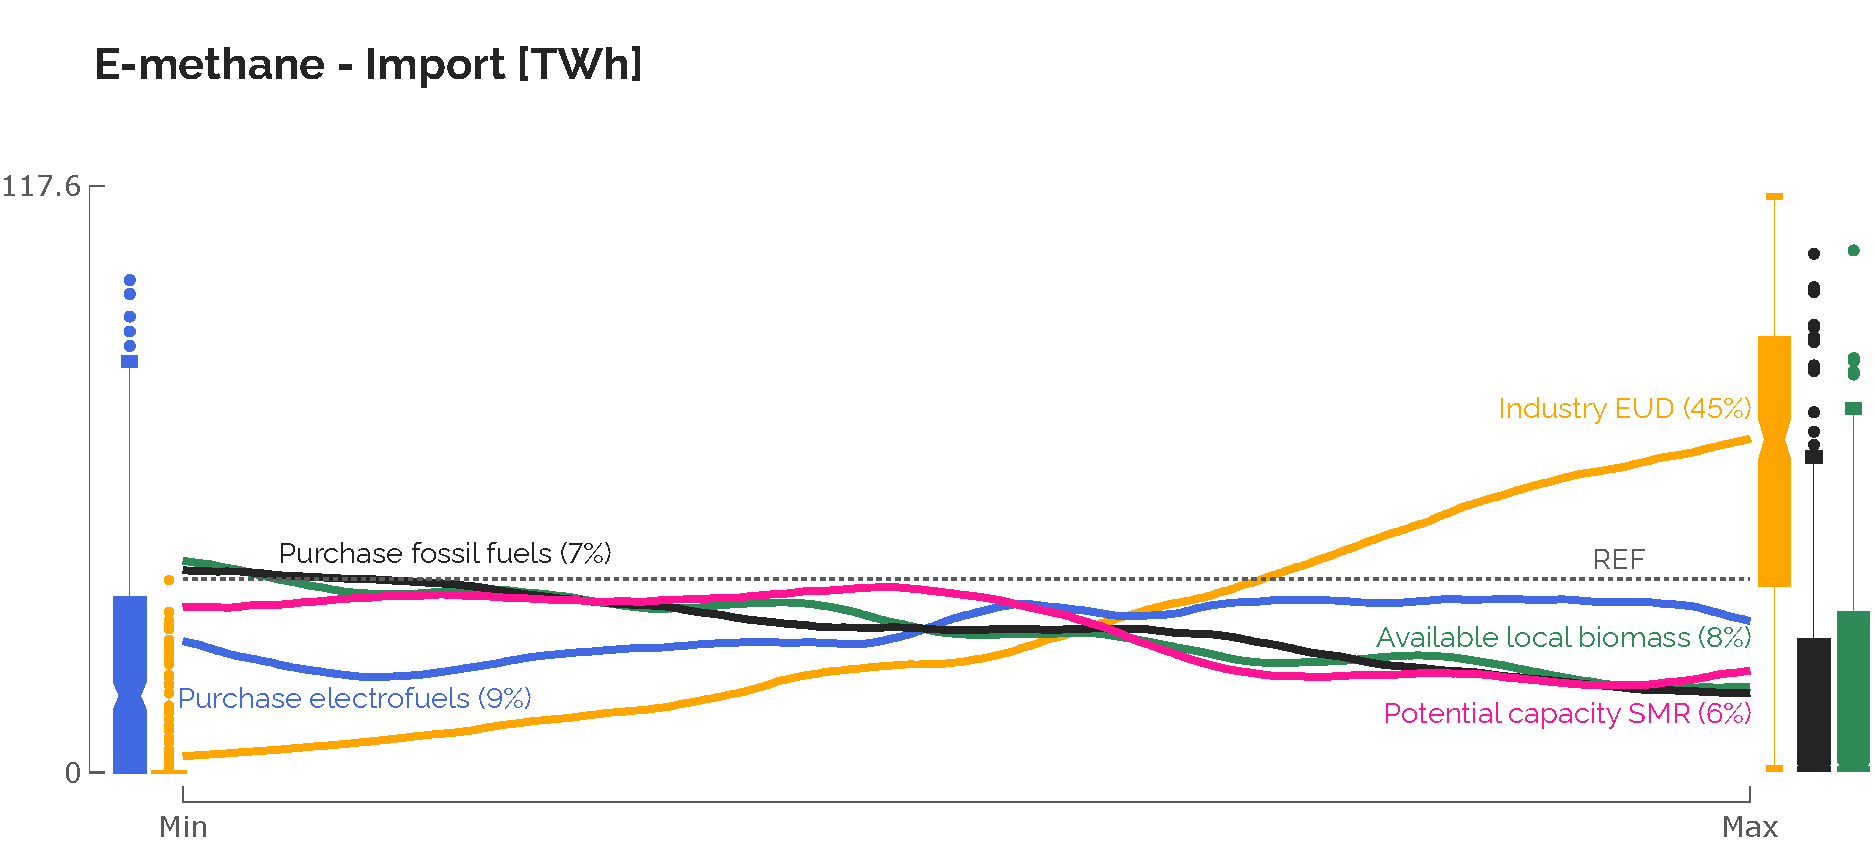
\includegraphics[width=0.8\textwidth]{UQ_Gas_samples_2.pdf}
\caption{Trend lines of the key parameters (and their Sobol' index) on the import of e-methane in 2050. Around these lines, box plots point out the distribution of the output of interest for the extreme values (either bottom-15\% or top-15\%) of some parameters. The grey dashed line gives the value of the output of interest in the REF case. }
\label{fig:results_uq_samples_gas}
\end{figure}

For the installed capacity of \gls{SMR}, it is the availability of the technology that drives its installation (Figure \ref{fig:results_uq_samples_SMR}). Not shown here but all the samples of the \gls{GSA} highlight that \gls{SMR} is installed to its maximum capacity, \ie 6\,GW, as soon as possible. In other words, the only parameter ``Potential capacity \gls{SMR}'' dictates the installation of this technology. In practice, we observe that as soon as this parameter is equal or higher than 0.9, 0.8 and 0.6, 6\,GW \gls{SMR} is installed from 2040, 2045 and 2050, respectively. The large range of uncertainty of its CAPEX (-40\%; +44\%) has a negligible impact on the installed capacity, with a Sobol' index of 0.9\%. This is explained by the long lifetime of the technology (60 years) and the salvage value recovered by 2050.

\begin{figure}[htbp!]
\centering
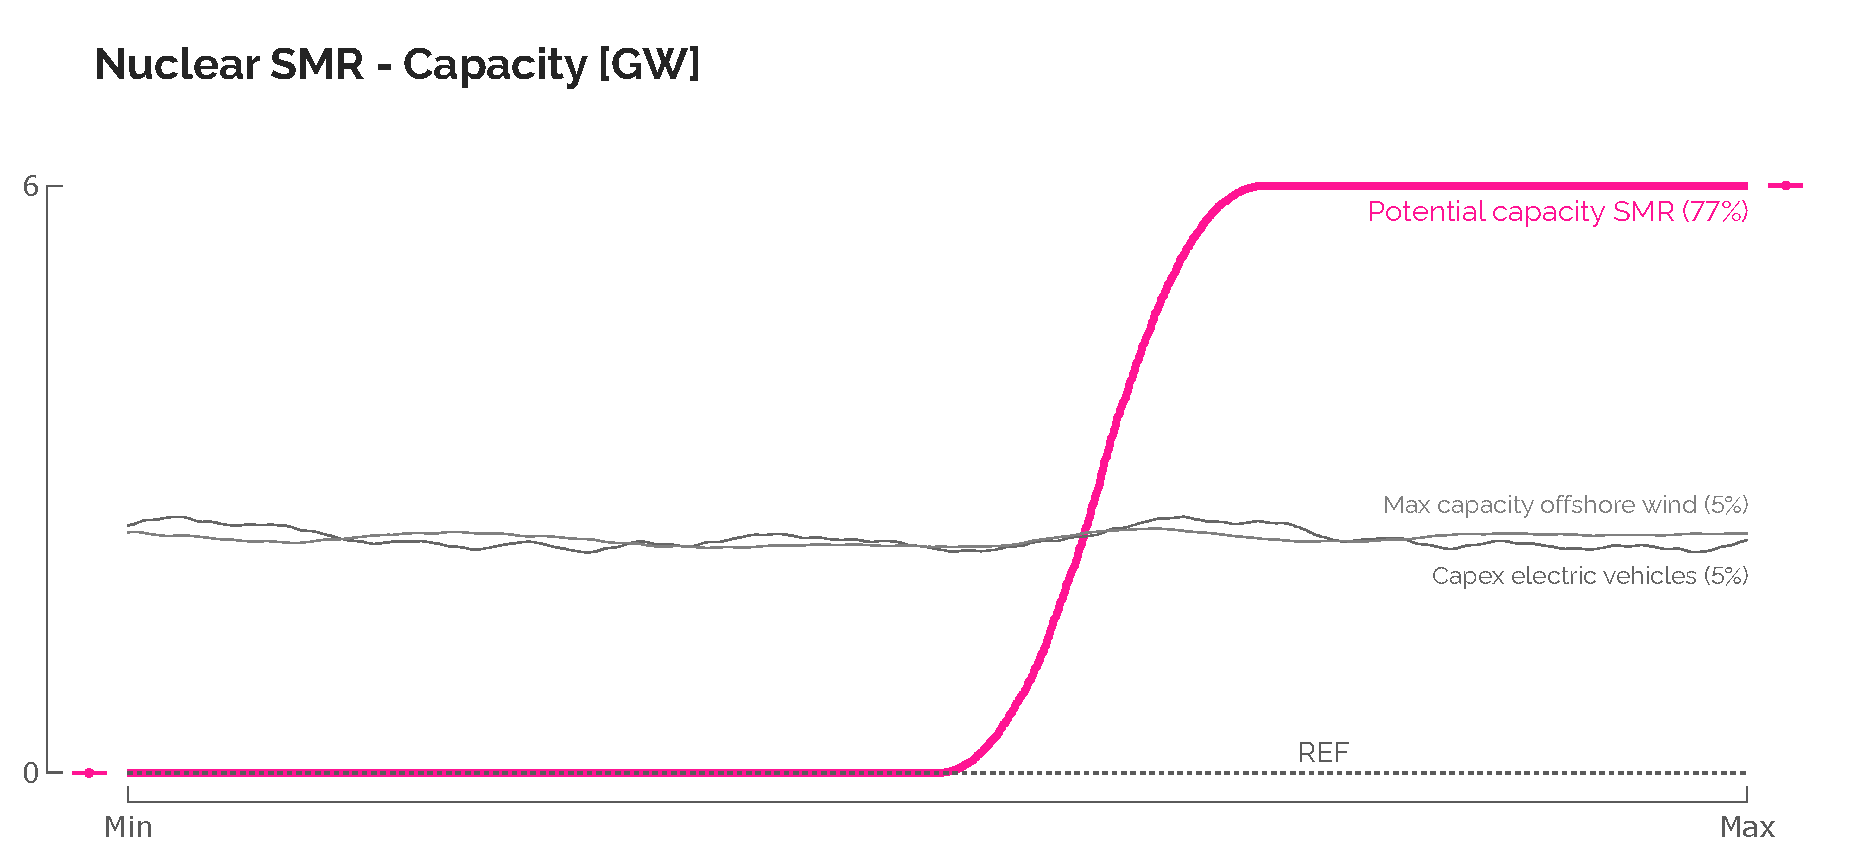
\includegraphics[width=0.8\textwidth]{UQ_SMR_samples_2.pdf}
\caption{Trend lines of the key parameters (and their Sobol' index) on the installed capacity of \gls{SMR} in 2050. Around these lines, box plots point out the distribution of the output of interest for the extreme values (either bottom-15\% or top-15\%) of some parameters. The grey dashed line gives the value of the output of interest in the REF case. }
\label{fig:results_uq_samples_SMR}
\end{figure}

\subsubsection{Local renewables}
\label{subsubsec:atom_mol:results_uq_VRES}
In line with the results given in Section \ref{subsec:atom_mol:results_deter}, the \gls{GSA} shows that \gls{SMR} has a negligible impact on the deployment of local \gls{VRES} (\ie \gls{PV}, onshore and offshore wind turbines). Whereas the installed capacities of onshore wind is totally driven by the uncertainty on its maximum potential, Sobol' indices change for the most impacting parameters on the deployment of \gls{PV} and offshore wind (see Figure \ref{fig:results_uq_pdf_local_ren}). The key factor that drives the installed capacities of these two technologies is mostly their respective maximum potential, especially at the end of the transition, much more than their CAPEX. Given its higher \gls{LCOE} (\Cref{fig:LCOE}), \gls{PV} is more impacted in the short term by the variation in the cost of purchasing electrofuels supplying e-methane (and e-ammonia to a lesser extent) \gls{CCGT}. However, this impact becomes negligible by 2050.

\begin{figure}[htbp!]
\centering
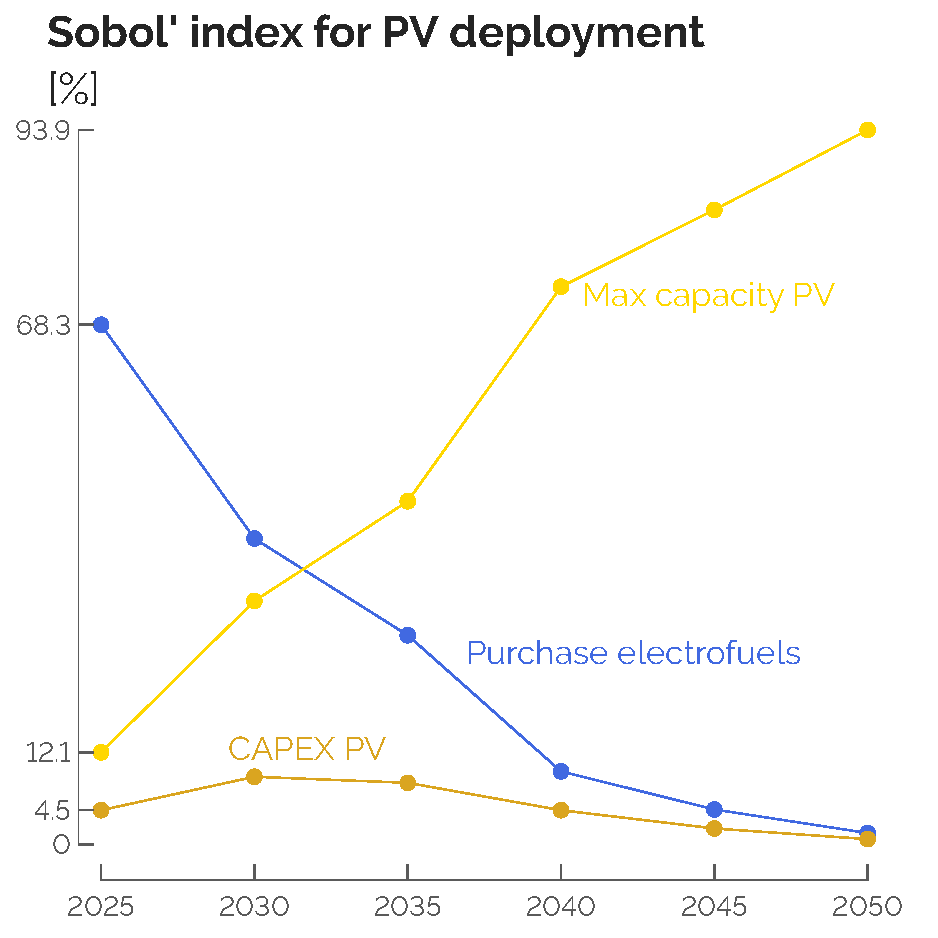
\includegraphics[width=0.49\textwidth]{Sobol_PV.pdf}
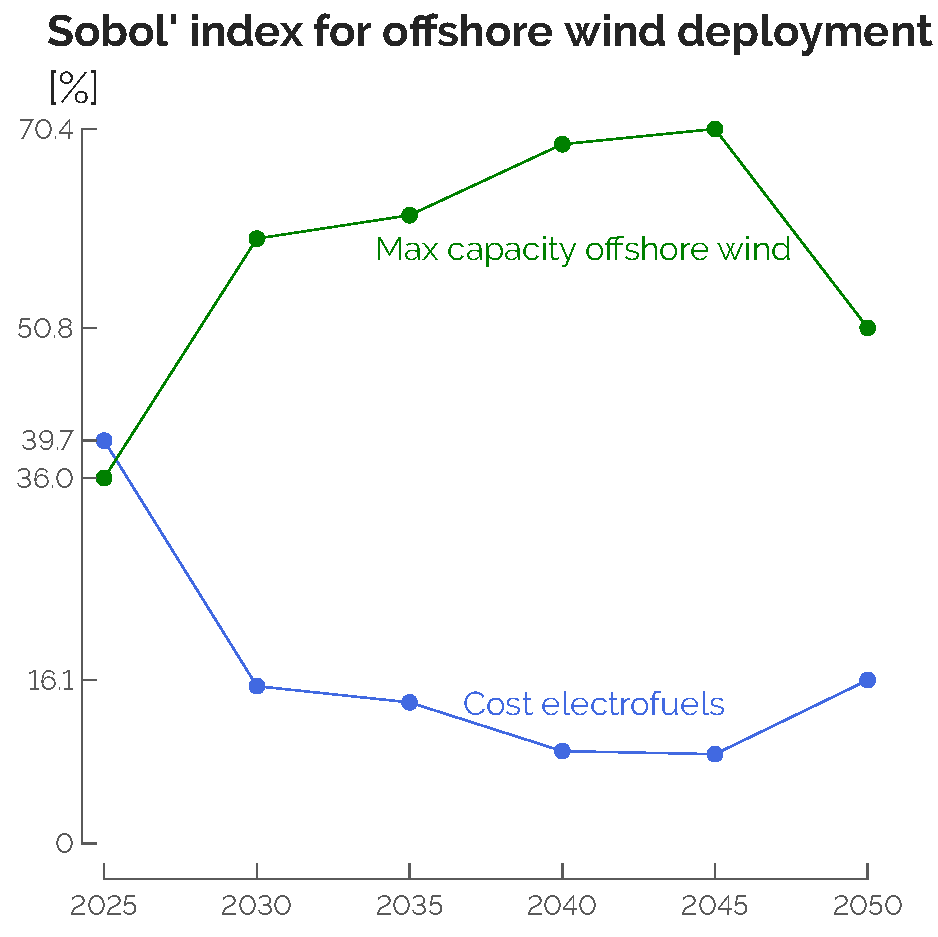
\includegraphics[width=0.49\textwidth]{Sobol_WIND_OFFSHORE.pdf}
\caption{Parameters impacting the deployment of \gls{PV} and offshore wind over the transition. Progressively, the impact of the uncertainty on the maximum potential increases, unlike the one on the cost of purchasing electrofuels.}
\label{fig:results_uq_pdf_local_ren}
\end{figure}


\newpage
\section{Interpretations and discussions}
\label{sec:discussions}
List here the key-messages:
\begin{itemize}
\setlength\itemsep{1em}
    \item Given its lower \gls{LCOE}, \gls{SMR} is installed as soon as available. It directly substitutes other flexible power generation units (\ie CCGT) and provides, by 2050, 44.6\,TWh, 25\% of the total electricity production. Consequently, this  reduces the need to produce electricity via \gls{CHP} and allows increasing by 48\% the high-temperature heat produced by electric heaters. Besides these two sectors, the others (\ie low-temperature heat, mobility and non-energy demand) are marginally or not impacted by the integration of \gls{SMR}.
    \item Betting on \gls{SMR} means letting the emissions go up at early stages of the transition (\ie \gls{LFO} still used in 2025 to produce \gls{HVC}) to end up with an overall transition and system by 2050 that are respectively 3.3\% and 8.8\% cheaper than the REF case. 
    \item Given the ambitious \ce{CO2}-budget (\ie 30-year budget representing 10 years of the current emissions), \acrfull{GSA} highlights the biggest impact of the cost of purchasing electrofuels on the variation of the total transition cost, around 45\%. On the contrary, parameters directly related to \gls{SMR} (\ie its availability and its CAPEX) have limited impact, below 1\%.
    \item Finally, the same \gls{GSA} points out the key drivers for the import of renewable electrofuels and the installation of \gls{SMR} by 2050. Besides the cost of purchasing electrofuels (\ie the lower this cost, the bigger the imports), it shows that available \gls{SMR} would have mainly a direct impact on e-ammonia, by substituting the ammonia \gls{CCGT} that is the biggest consumer of this molecule. Indirectly, this parameter will also reduce the import of e-methane by reducing the need for gas \gls{CHP} and gas boilers. About e-hydrogen and e-methanol, their imports are impacted by the other technologies in competition in the transport sector and the industrial demand, respectively.
    \item ``In other words, \gls{SMR} competes with importing electrofuels while both support the integration of local solar and wind energies.'' from Section \ref{subsubsec:results_deter_overall}
\end{itemize}

%%%%%%%%%%%%%%%%%%%%%%%%%%%%%%%%%%%%%%%%%%%%%%%%%%%%%%%%%%%%%%%%%%%%%%%%%%%%%%%%%%%%%%%%%%%%%%%%%%%%%%%%%%%%%%%%%%%%%%%%%%%%%           CONCLUSION %%%%%%%%%%%%%%%%%%%%%%%%%%%%%%%%
%%%%%%%%%%%%%%%%%%%%%%%%%%%%%%%%%%%%%%%%%%%%%%%%%%%%%%%%%%%%%%%%%%%%%%%%%%%%%%%%%%%%%%%%%%%%%%

\section{Conclusions and further works}
\label{sec:conclusion}
\textbf{Quid autre que techno-economic Nucléaire-SMR?}
\textbf{Quid demande plus faible?}
\textbf{Quid importation massive de molécules}
Hervé Kempf - \url{https://www.seuil.com/ouvrage/le-nucleaire-n-est-pas-bon-pour-le-climat-herve-kempf/9782021512922}

\begin{itemize}
    \item Other dimensions to consider: societal, etc.
    \item Reducing the demand. Refer to Hugo Baudson \cite{baudson2022impact}
    \item Will we be able to import as many molecules as we need? Refer to \cite{lefebvre2022electrofuel}.
\end{itemize}

Parier sur l'arrivée du \gls{SMR} peut être considéré comme une fuite vers l'avant quant à l'abandon des ressources fossiles, (to a lesser extent) mais ne touche pas (ou presque) au déploiement du renouvelable local, vers moins de sector coupling (moins de CHP), Less efficiency

A significant decrease on the demand-side is probably one of the cornerstones of the energy transition \cite{millward2020providing, contino_sobriety}.

comparaison avec \cite{heuberger2018impact} et \cite{PATHS2050}

Relying on nuclear would not especially increase our national self-sufficiency, on the contrary (more import of energy in general, by 2050)

Discussion on the \ce{CO2}-budget allocated to Belgium that could/should be lower to allow other countries in development reaching the floor of the donuts (donuts theory) $-->$ reducing the demand?

6GW, ça ne représente qu'une petite partie du problème

\textbf{Further works}
\begin{itemize}
    \item Quid si on attend (same strat jusque 2040) et que finalement, il n'arrive jamais. Quel serait le surcoût? La surconso d'électrofuels. Intéressant de mettre en place une policy robuste pour parer cette éventualité, surtout étant donné la vision plus myopique des choses $-->$ Reinforcement learning
    \item Analyse what the system looks like in the extreme cases where the imports are massive
\end{itemize}


\begin{appendices}
%%%%%%%%%%%%%%%%%%%%%%%%%%%%%%%%%%%%%%%%%%%%%%%%%%%%%%%%%%%%%%%%%%%%%%%%%%%%%%%%%%%%%%%%%%%%%%%%%%%%%%%%%%%%%%%%%%%%%%%%%%%%%           APP METHODO 		 %%%%%%%%%%%%%%%%%%%%%%%%%%%%%%%%%%%%%%%%%%%%%%%%%%%%%%%%%%%%%%%%%%%%%%%%%%%%%%%%%%%%%%%%%%%%%%%%%%%%%%%%%%%%%%%%%%%%%%%%%%%%%%

\section{Methodology}
\label{sec:methodo}
The core of this section is, on the one hand, to introduce the model used in this analysis, EnergyScope Pathway \cite{limpens2024pathway} and, on the other hand, to introduce the framework that assesses the impact of uncertainties on the output of interest of the model (\eg total transition cost, amount of imported electrofuels or installed capacity of \gls{SMR}). To do so, the second part of this section focuses on the uncertainty characterisation developed by \citet{Moret2017} and the uncertainty quantification using \acrfull{PCE} \cite{Sudret2014}.

\subsection{EnergyScope Pathway}
\label{subsec:meth:ES_Pathway}
In a previous work, \citet{rixhon2021role} set different emission constraints on the snapshot model, \gls{ESTD} \cite{limpens2019energyscope}, for the target future year of 2050. On the contrary, this work optimises the entire transition pathway from a known system in 2020 up to 2050 thanks to EnergyScope Pathway \cite{limpens2024pathway}. According to pathway models review, EnergyScope Pathway can be categorised as an investment and operation optimisation model that assesses the whole-energy system, has a hourly time-resolution and is open-source documented model. Moreover, it maintains a low computational cost (\ie around 15 minutes for a 30-year pathway with a hourly discretisation). Presenting here only the main constraints of the model and the main input data in Appendix \ref{app:case_study}, the reader is invited to refer to the extended paper \cite{limpens2024pathway} and the documentation \cite{readthedocs_pathway} for more extensive information.

\begin{figure}[htbp!]
\centering
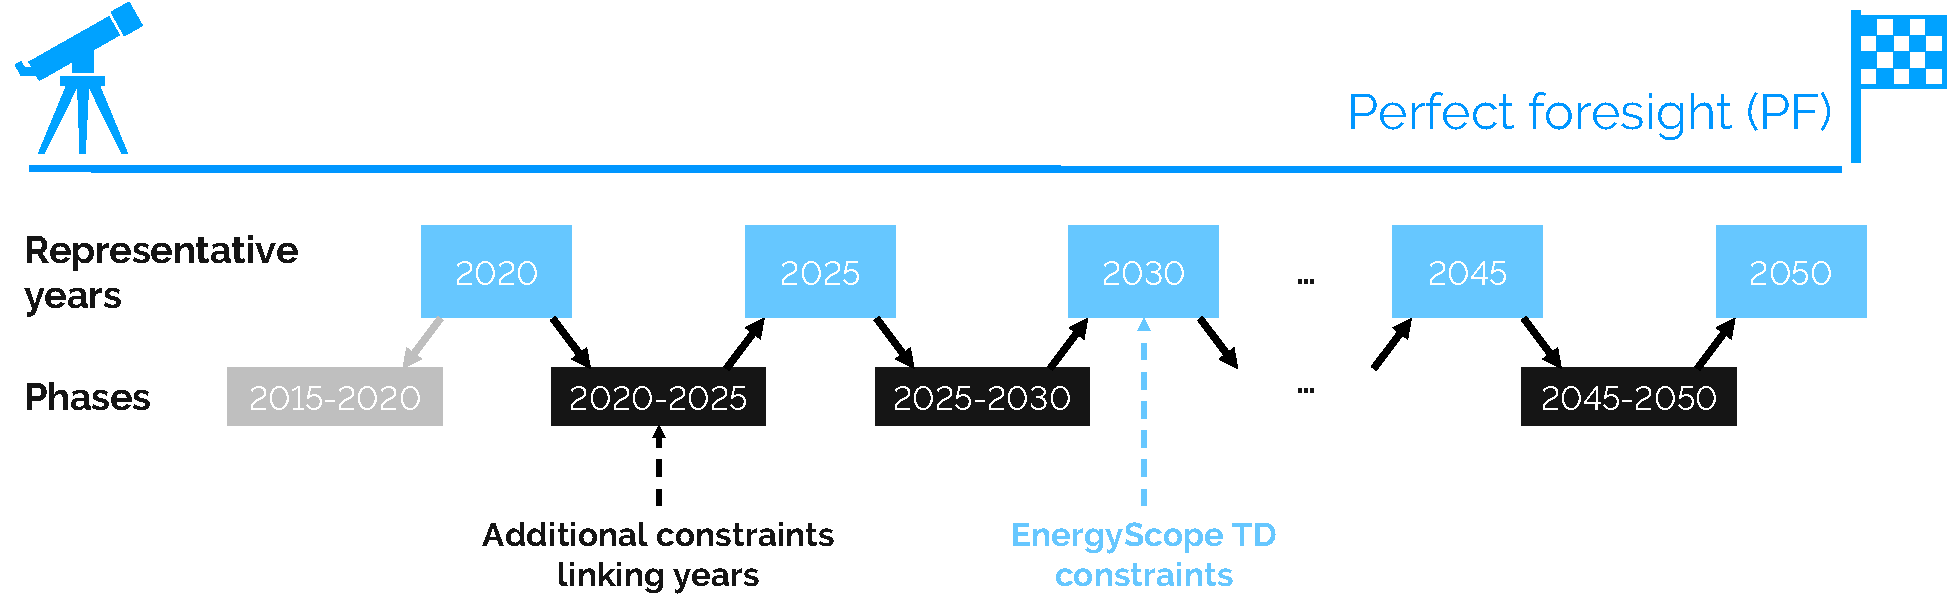
\includegraphics[width=\textwidth]{ES_Pathway.pdf}
\caption{Illustration of the pathway methodology based on an existing energy system model. The methodology spans from 2020 to 2050, with one representative year every five years. The model \acrfull{ESTD} is applied in 7 representative years (light blue boxes). The formulation includes additional constraints (black boxes) that link the years together. The pathway's initialisation assumes that all capacities installed in 2020 were built during the pseudo-phase of 2015-2020 (grey box). The overall problem is defined as the pathway model. Graph adapted from \cite{limpens2024pathway}.}
\label{fig:meth_path_methodology}
\end{figure}

We used the perfect foresight (PF) formulation (\Cref{fig:meth_path_methodology})---the entire transition is computed in one optimisation, assuming a complete but uncertain knowledge of the different parameters until 2050. Even though this lacks realism compared to the myopic approach \cite{babrowski2014reducing,fais2016impact,heuberger2018impact} where the pathway is optimised via a sequence of shorter time windows, the perfect foresight approach allows to optimise the transition with a \ce{CO2}-budget (Section \ref{subsec:cs:CO2-budget}) rather than along a prescribed \ce{CO2}-trajectory. However, the work of \citet{limpens2024pathway} has shown that PF provides similar results for the study case compared to the myopic approach with a prescribed linear decrease of the \ce{CO2}-emissions . All the variables and constraints of the snapshot model, EnergyScope TD \cite{limpens2019energyscope}, are kept as is with an extra-dimension to relate them to a specific representative year, $y$, of the pathway. For instance, the energy balance is guaranteed at every hour of each of these years. 

The optimised objective of the pathway model, \ie the total transition cost $\textbf{C\textsubscript{tot,trans}}$, is computed as follows: 

\begingroup
\belowdisplayskip=2pt
\abovedisplayskip=2pt
\begin{flalign} 
% Objective function + investment 
\label{eq:obj_func_v2}%1
% adding 25pt space, otherwise flalign with two "&" would flush to the extreme 
\hspace{0pt} \min \text{  } & \textbf{C\textsubscript{tot,trans}} = \textbf{C\textsubscript{tot,capex}} + \textbf{C\textsubscript{tot,opex}}&\\
\label{eq:CAPEX_v2}
& \textbf{C\textsubscript{tot,capex}} =
\sum_{\mathclap{p \in \text{\emph{PHASE}}\cup \{2015\_2020\}}} 
\textbf{C\textsubscript{inv,phase}}(p)
-
\sum_{\mathclap{j \in \emph{TECH}}} 
\textbf{C\textsubscript{inv,return}}(j)\\
  \label{eq:Copex_tot_v2}%5
& \textbf{C\textsubscript{tot,opex}} =  \textbf{C\textsubscript{opex}}(2020)
+ \emph{t\textsubscript{phase}}\cdot \tau\textsubscript{\emph{phase}}(p) \cdot \sum_{\mathclap{p \in \emph{PHASE}|y\textsubscript{start}\in \emph{P\_START}(p),y\textsubscript{stop}\in \emph{P\_STOP}(p)}} 
 \Big(\textbf{C\textsubscript{opex}}(y\textsubscript{start}) + \textbf{C\textsubscript{opex}}(y\textsubscript{stop}) \Big)/2&\\
\label{eq:path_annu_factor}
& \tau\textsubscript{\emph{phase}}(p) = 1/(1+\emph{i\textsubscript{rate}})^{\emph{diff\_2015\_year(p)}} &
%% GL_correction_v2 %% & \tau\textsubscript{\emph{phase}}(p) = 1/(1+\emph{i\textsubscript{rate}})^{\emph{diff\_2015\_year(p)}} &
\end{flalign}
\endgroup

\noindent
where $\emph{t\textsubscript{phase}}=5\,\text{years}$ and $\emph{diff\_2015\_year(p)}$ are respectively the duration of a phase between two representative years and the number of years between the middle of a phase and 2015 for a correct annualisation. $\textbf{C\textsubscript{inv,return}}$ accounts for the residual value, also called \textit{salvage value}, of the technologies installed during the transition and having not reached the end of their lifetime by 2050. This last variable is crucial to avoid penalising heavy (and potentially long-lifetime) investments at the end of the transition as these assets would still be operational beyond 2050. The interested reader will find more information about its implementation and the formulation choices related to it in the work of \citet{limpens2024pathway}. The other variables in Eq.\,(\ref{eq:CAPEX_v2}-\ref{eq:Copex_tot_v2}) are detailed here below:

\begingroup
\belowdisplayskip=2pt
\abovedisplayskip=2pt
\begin{flalign} 
\label{eq:opex_yearly}
&\textbf{C\textsubscript{opex}} (y) = \sum_{\mathclap{j \in \emph{TECH}}} \textbf{C\textsubscript{maint}}(y,j) + \sum_{\mathclap{i \in \emph{RES}}} \textbf{C\textsubscript{op}}(y,i)&\forall y\in \emph{YEARS}\\
\label{eq:PhaseInv}%5
&\textbf{C\textsubscript{inv,phase}}(p) = \sum_{\mathclap{j \in \emph{TECH}}} \textbf{F\textsubscript{new}}(p,j)\cdot \tau\textsubscript{\emph{phase}}(p)\cdot \left(\emph{c\textsubscript{inv}}(\emph{y\textsubscript{start}},j) + \emph{c\textsubscript{inv}}(\emph{y\textsubscript{stop}},j)\right)/2&\notag\nonumber
\end{flalign}
\begin{flalign}
&&\forall p \in \emph{PHASE} | y\textsubscript{start}\in \emph{P\_START}(p),y\textsubscript{stop}\in \emph{P\_STOP}(p)
\end{flalign}
\endgroup

\noindent
where $\textbf{F\textsubscript{new}}$ are the capacities newly installed. In Eq. (\ref{eq:opex_yearly}-\ref{eq:PhaseInv}), the costs related to each representative year are:

\begingroup
\belowdisplayskip=2pt
\abovedisplayskip=2pt
\begin{flalign} 
% Objective function + investment 
% adding 25pt space, otherwise flalign with two "&" would flush to the extreme left
\hspace{0pt} 
 \label{eq:c_inv}%3
 &\textbf{C\textsubscript{inv}}(y,j) = c_{\text{\emph{inv}}}(y,j) \textbf{F}(y,j) & \forall y \in \text{\emph{YEARS}}, \forall j \in \text{\emph{TECH}}\\
 \label{eq:c_maint}%4
 &\textbf{C\textsubscript{maint}}(y,j) = c_{\text{\emph{maint}}}(y,j) \textbf{F}(y,j) & \forall y \in \text{\emph{YEARS}}, \forall j \in \text{\emph{TECH}}\\ 
  \label{eq:c_op}%5
 &\textbf{C\textsubscript{op}}(y,i) = \sum_{\mathclap{t \in T }} c_{\text{\emph{op}}}(y,i) \textbf{F\textsubscript{t}}(y,i,t) t_{op} (t)  
 & \forall y \in \text{\emph{YEARS}}, \forall i \in \text{\emph{RES}}
 \end{flalign}
 \endgroup

\noindent where the variable $\textbf{F}$ represents the size of the installed capacities (for all technologies $j$) and the variable $\textbf{F\textsubscript{t}}$ is the hourly consumption of the resources; the parameters $c_{\text{\emph{inv}}}$ and $c_{\text{\emph{maint}}}$ are the CAPEX and the OPEX of the technologies, and the parameter $c_{\text{\emph{op}}}$ is the cost of purchasing resources. For the sake of simplicity, as done by \citet{limpens2024pathway}, the sum over the 8760 hours of the year is written as the sum over $t \in T $. 

Then, as detailed in section \ref{subsec:cs:CO2-budget}, the \ce{CO2}-budget for the transition, $\textbf{GWP\textsubscript{tot,trans}}$, is computed and constrained as follows:

\begingroup
\belowdisplayskip=2pt
\abovedisplayskip=2pt
\begin{flalign} 
\label{eq:gwp_tot_transition}
&\textbf{GWP\textsubscript{tot,trans}}= \textbf{GWP\textsubscript{tot}}(2020) + \emph{t\textsubscript{phase}}\sum_{\mathclap{p \in \emph{PHASE}|y\textsubscript{start}\in \emph{Y\_START}(p),y\textsubscript{stop}\in \emph{Y\_STOP}(p)}}\left(\textbf{GWP\textsubscript{tot}}(y\textsubscript{start}) +\textbf{GWP\textsubscript{tot}}(y\textsubscript{stop}) \right)/2 &
\\
\label{eq:limit_gwp_trans}
& \textbf{GWP\textsubscript{tot,trans}} \leq \emph{gwp\textsubscript{lim,trans}}&
\end{flalign}
\endgroup

\noindent
where the computation of the yearly emissions are based on the \acrfull{GWP} of the resources:

\begingroup
\belowdisplayskip=2pt
\abovedisplayskip=2pt
\begin{flalign}
\hspace{0pt}
 \label{eq:GWP_tot}%8
 & \textbf{GWP\textsubscript{tot}}(y)  =    \sum_{\mathclap{i \in \text{\emph{RES}}}} \textbf{GWP\textsubscript{op}}(y,i) 
 & \forall y \in \text{\emph{YEARS}}\\
  \label{eq:GWP_op}%7
 & \textbf{GWP\textsubscript{op}}(y,i) = \sum_{\mathclap{t \in T }} gwp_{\text{\emph{op}}}(y,i) \textbf{F\textsubscript{t}}(y,i,t)  t_{op} (t) & \forall y \in \text{\emph{YEARS}}, \forall i \in \text{\emph{RES}}
\end{flalign}
\endgroup

\noindent
where $gwp_{\text{\emph{op}}}$ is the specific emissions (\ie in kt$_{\ce{CO2},\text{eq}}$/GWh) of each resource. Based on an approach developed by the Intergovernmental Panel on Climate Change (IPCC) \cite{stocker2014climate}, this work considers the indicator ``GWP100a - IPCC2013'' to compute the emissions related to the use of resources. This includes the emissions due to the extraction, the transportation and the combustion of the energy carrier. EnergyScope proposes to account for the embodied emissions of the technologies based on a \gls{LCA}. These stand for extraction of materials, refining, construction and end of life \cite{schnidrig2023integration}. However, this work is still in progress and the database is not yet complete. Consequently, it is not included in this work and not accounted for.

Besides this constraint on the emissions, the main constraint to link years with each other is the one dictating the installed capacities at the end of each year:

\begingroup
\belowdisplayskip=2pt
\abovedisplayskip=2pt
\begin{flalign} 
\label{eq:F_newBuilt}%5
&\textbf{F}(y\textsubscript{stop},j) = \textbf{F}(y\textsubscript{start},j)
 + \textbf{F\textsubscript{new}}(p,j)
 - \textbf{F\textsubscript{old}}(p,j)
 - \sum_{\mathclap{p2 \in \text{\emph{PHASE}} \cup \{2015\_2020\}}} \textbf{F\textsubscript{decom}}(p,p2,j)& \notag \nonumber 
 \end{flalign}
\begin{flalign} 
 &&  \forall p \in \text{\emph{PHASE}}, \emph{y\textsubscript{stop}} \in \emph{Y\_STOP}(p), \emph{y\textsubscript{start}} \in \emph{Y\_START}(p), j \in \text{\emph{TECH}}
 \end{flalign}
\endgroup

\noindent
where the variables $\textbf{F\textsubscript{old}}$ and $\textbf{F\textsubscript{decom}}$ are the capacities respectively having reached the end of their lifetime and prematurely decommissioned. Moreover, to account for the society inertia and to prevent unrealistically fast modal share change, constraints limit this change for the sectors of the low-temperature, the passenger mobility and freight mobility demands. The parameters $\Delta_{\mathrm{change,LT\_heat}}$, $\Delta_{\mathrm{change,pass}}$ and $\Delta_{\mathrm{change,freight}}$ respectively limit their respective modal share change up to 33\%, 50\% and 50\% per phase of 5 years.

\subsection{Uncertainty quantification}
\label{subsec:meth:UQ}
In their systematic review, \citet{yue2018review} highlighted that a wide majority of studies addressing the optimisation of energy systems (\ie 75\% out of the 134 reviewed studies) were not investigating the impact of uncertainties. However, disregarding these impacts can have drastic consequences on the system design. For instance, historical low \gls{NG} prices have led to overcapacity of \gls{CCGT} in Europe \cite{moret2020overcapacity}. This is why accounting for uncertainty in \gls{ESOM} is crucial \cite{mavromatidis2018uncertainty}, especially when it comes to optimise several decades in an inherently uncertain future \cite{peace2008insights}.

This section aims at briefly presenting the methods followed to first characterise these uncertainties, then to quantify their impact on different outputs of interest of the model (\eg amount of molecules imported from abroad, the installed capacity of \gls{SMR} or the total transition cost) and finally, the screening and selection of the parameters to analyse.

\subsubsection{Uncertainty characterisation and sampling}
\label{subsubsec:UQ:UC}
Characterising precisely the uncertainty---ideally with their respective probability density functions (PDFs)---of the thousands of parameters in the model is daunting if not impossible because of lack of data \cite{marnay2006addressing}. Therefore, we used a workaround developed by \citet{Moret2017} that defines relative ranges of variation for different groups of parameters. These ranges have been adapted for the Belgian energy system and the pathway formulation. Moreover, some ranges have been added to account for new parameters coming from the pathway formulation described in \Cref{subsec:meth:ES_Pathway} like the society inertia.

\Cref{tab:UC_short} gives the uncertainty ranges of some key parameters. Like other works \cite{li2019renewables,coppitters2021robust}, the uncertain parameters are assumed to be independent and uniformly distributed between their respective lower and upper bounds. A particular attention is to pay to the potential installation of \gls{SMR}, at the bottom of \Cref{tab:UC_short}. As detailed in Appendix \ref{app:case_study}, the commercial availability of such a technology is uncertain but would not be before 2040. Consequently, for \gls{SMR}, the parameter $f_{\mathrm{max,SMR}}$ influences the maximum capacity to install to translate somehow the readiness of this technology. As SMRs are foreseen, if installed, to be around the same locations (\ie Tihange and Doel) as the conventional nuclear power plants and using the same area in kW/ha, the same 6\,GW are assumed to be the maximum capacity for SMRs. If it is (i) smaller than 0.6, there is no possibility to install \gls{SMR} during the transition; (ii) between 0.6 and 0.8, these 6~GW can be installed only in 2050; (iii) between 0.8 and 0.9, these can be installed from 2045 onward and; (iv) higher than 0.9, the prescribed maximum capacity can be installed from 2040 onward. Based on the local sensitivity analysis carried out by \citet{PATHS2050}, the current work also considers a [-40\%; +44\%] range on the CAPEX of SMR, on top of the uncertainty about the availability. Finally, the the cost of purchasing renewable electrofuels presents a wide range, [-64.3\%; +179.8\%], like the other imported commodities.

The exhaustive list of the parameters accounted in this work is presented in Appendix \ref{subsec:cs:uncertainty}.

\begin{table}[htbp!]
\caption{Illustration of the uncertainty characterisation for different parameters for the year 2025. $^{(a)}$ Per \cite{Moret2017PhDThesis}, \og I: investment-type, II: operation-type (constant uncertainty over time), III: operation-type (uncertainty increasing over time)\fg. $^{(b)}$ The nominal value of each parameter is 0, meaning no variation compared to the nominal values of the impacted parameter in the model. $^{(c)}$ This range has been inferred from the local sensitivity analysis performed by \citet{PATHS2050}.}
\label{tab:UC_short}
\centering
\resizebox{\textwidth}{!}{
\begin{tabular}{l l l c c c}
\toprule
\multirow{2}{*}{\textbf{Category}} & \multirow{2}{*}{\textbf{Parameter}} & \multirow{2}{*}{\textbf{Meaning}} & \multirow{2}{*}{\textbf{Type}$^{(a)}$}  & \multicolumn{2}{c}{\textbf{Relative variation$^{(b)}$}}\\
    & & & &	 min 	&	 max \\ 	
\midrule		
\multirow{2}{*}{\textbf{Cost of purchasing}} & $c_{\mathrm{op,fossil}}$ & Purchase fossil fuels & II & -64.3\% & 179.8\% \\
& $\bm{c_{\mathrm{op,electrofuels}}}$ & \textbf{Purchase electrofuels} & \textbf{II} & \textbf{-64.3\%} & \textbf{179.8\%} \\
\midrule
\multirow{5}{*}{\textbf{Investment cost}} &$c_{\mathrm{inv,car}}$ & CAPEX car  & I & -21.6\% & 25.0\% \\
& $c_{\mathrm{inv,e\_prop}}$ & CAPEX electric motor & I & -39.6\% & 39.6\% \\
& $c_{\mathrm{inv,fc\_prop}}$ & CAPEX fuel cell engine & I & -39.6\% & 39.6\% \\
& $c_{\mathrm{inv,PV}}$ & CAPEX PV & I & -39.6\% & 39.6\% \\
& $\bm{c_{\mathrm{inv,nuclear\_SMR}}}$ & \textbf{CAPEX \gls{SMR}}$^{(c)}$ & \textbf{I} & \textbf{-40.0\%} & \textbf{44.0\%} \\
\midrule
\multirow{1}{*}{\textbf{Consumption}} &$\eta_{\mathrm{e\_prop}}$ & Consumption electric vehicles & I & -28.7\% & 28.7\% \\
\midrule
\multirow{3}{*}{\textbf{Potential installed capacity}} &$f_{\mathrm{max,PV}}$ & Max capacity PV & I & -24.1\% & 24.1\% \\
& $f_{\mathrm{max,windon}}$ & Max capacity onshore wind & I & -24.1\% & 24.1\% \\
& $\bm{f_{\mathrm{max,SMR}}}$ & \textbf{Potential capacity \gls{SMR}} & \textbf{-} & \textbf{0} & \textbf{1} \\
\midrule
\multirow{2}{*}{\textbf{Hourly load factor}} & $c_{\mathrm{p,t,PV}}$ & Hourly load factor PV & II & -22.1\% & 22.1\% \\
& $c_{\mathrm{p,t,winds}}$ & Hourly load factor wind turbines & II & -22.1\% & 22.1\% \\
\midrule
\multirow{2}{*}{\textbf{Resource availability}} & $avail_{\mathrm{elec}}$ & Available electricity import & I & -32.1\% & 32.1\% \\
& $avail_{\mathrm{biomass}}$ & Available local biomass & I & -32.1\% & 32.1\% \\
\midrule

\multirow{2}{*}{\textbf{End-use demand}} & $pass\_EUD$ & Passenger mobility EUD & III & -7.5\% & 7.5\% \\
& $industry\_EUD$ & Industry EUD & III & -20.5\% & 16.0\% \\
\midrule

\multirow{3}{*}{\textbf{Miscellaneous}} &$i_{\mathrm{rate}}$  & Interest rate & I & -46.2\% & 46.2\% \\
& $\Delta_{\mathrm{change,freight}}$ & Modal share change freight mobility & - & -30\% & 30\% \\
& $\Delta_{\mathrm{change,pass}}$ & Modal share change passenger mobility & - & -30\% & 30\% \\


\bottomrule							

\end{tabular}}
\end{table}

Following the methodology defined by \citet{Moret2017}, uncertainties of types I (investment-type) and II (operation-type, constant uncertainty over time) keep the same range for the whole transition. However, parameters with an uncertainty increasing over time, type III, (\ie end-use demands, in this case) will have a wider and wider range over the transition. In this work, a +50\% linear increase has been arbitrarily set between the width of the range of such parameters in 2025 and the same ranges in 2050. In \Cref{fig:ranges_transition}, this means that for type III uncertainties only, $R_{2050}^+$ is 50\% bigger than $R_{2025}^+$ and $R_{2050}^-$ is 50\% smaller than $R_{2025}^-$. For uncertainties of types I and II, the relative variation versus the nominal value remain the same over the transition. Inspired by \citet{guevara2022modeling}, the values of the uncertain parameters are set at a fixed relative position from the nominal values for each sampled transition---the values do not zigzag from 2025 to 2050 within the bounds (\Cref{fig:ranges_transition}).

\begin{figure}[htbp!]
\centering
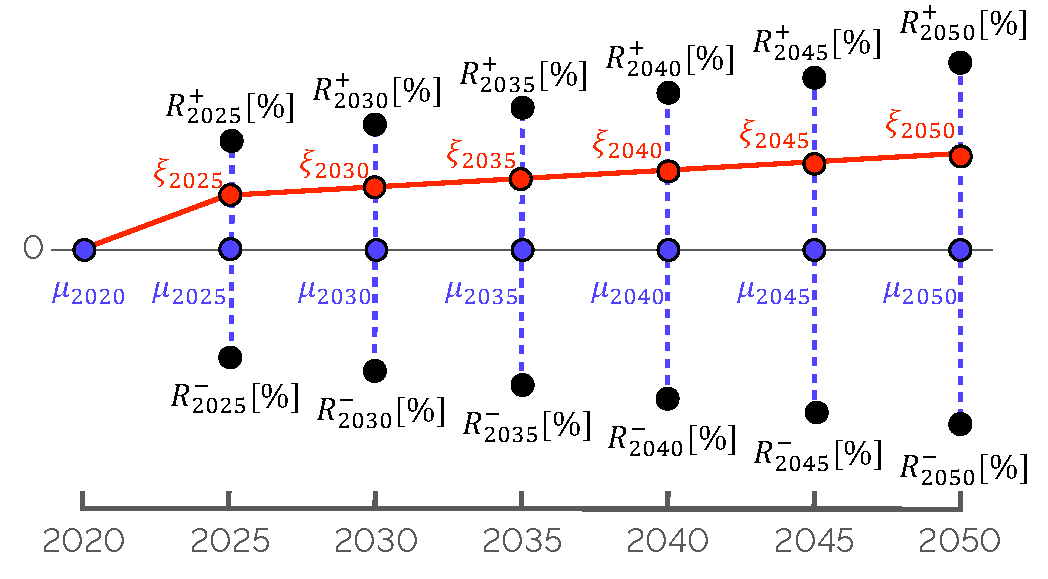
\includegraphics[width=0.5\textwidth]{ranges_transition.pdf}
\caption{$\mu_{2020}$, $\mu_{2025}$, ...,  $\mu_{2050}$ are the nominal values equal to 0 as the uncertain parameters represent a relative increase/decrease of actual parameters of the model. $R^+$ and $R^-$ are respectively the upper and lower bounds of the range and $\xi_{2025}$, $\xi_{2030}$, ...,  $\xi_{2050}$ are the values taken by one parameter for a specific sample of the \gls{GSA} for each of the representative years of the transition, always starting from the nominal value in 2020, $\mu_{2020}$. The graph has been adapted from \cite{guevara2022modeling}.}
\label{fig:ranges_transition}
\end{figure}

Finally, the model accounts for thousands of parameters. The computational burden to consider all of them separately would be completely overwhelming ($\sim 10^7$ model runs). Therefore, similarly to other works \cite{Moret2017,limpens2020impact}, the model parameters that would follow the same uncertainty have been grouped to one single uncertain parameter. For instance, the uncertainty on the cost of purchasing renewable electrofuels, $c_{\mathrm{op,electrofuels}}$, identically affects the cost of e-hydrogen, e-methane, e-ammonia and e-methanol. Indeed, besides their respective specificities, each of these fuels will be similarly affected by the variation of cost of electricity or the electrolyser, that drive the majority of their cost of purchasing \cite{h2coalition}. Similarly, the uncertainties impacting the industrial demand, $industry\_EUD$, alters equally the industrial high- and low-temperature and electricity demands as well as the non-energy demand.

\subsubsection{Polynomial Chaos Expansion}
\label{subsubsec:UQ:PCE}
We used \gls{PCE}, an approach for surrogate-assisted \gls{UQ}, to propagate uncertainties in input parameters through the system model. This allowed us to assess statistical moments on the quantity of interest and determine Sobol' indices~\cite{coppitters2020robust}. To construct a PCE of the EnergyScope Pathway model, we employed the open-source Python framework RHEIA~\cite{coppitters2022rheia,readthedocs_rheia}.\par

The PCE model ($\hat{M}$) is a representation of the relationship between the input parameters and the output variable of interest (\ie results) in the EnergyScope Pathway model ($M$). This representation is constructed as a truncated series of multivariate orthonormal polynomials $\bm{\Psi}$, weighted by coefficients $u$:

\begin{equation}
\hat{M} \left( \bm{\xi} \right) = \sum_{\bm{\alpha} \in \mathcal{A}^{d,p}} u_{\bm{\alpha}} \bm{\Psi}_{\bm{\alpha}} \left( \bm{\xi} \right) \approx M \left( \bm{\xi} \right), 
\end{equation}

where the vector $\bm{\xi} = (\xi_1,\xi_2, \dots \xi_d)$ comprises the independent random input parameters (see Appendix \ref{subsec:cs:uncertainty}), $d$ corresponds to the number of input distributions and $\bm{\alpha}$ is a multi-index, \ie a vector of non-negative indices of length $d$, where each index corresponds to the degree of each univariate polynomial that forms the basis of the multivariate polynomial $\bm{\Psi_{\bm{\alpha}}}$. As uniform distributions are considered, the Legendre polynomials are adopted, as they are the associated family of polynomials that are orthogonal with respect to standard uniform distributions~\cite{Sudret2014}.\par 

A truncation scheme is implemented to restrict the number of multivariate polynomials in the series. This is done based on two factors: a specified limiting polynomial order ($p$) and the number of uncertain parameters ($d$) involved. The multivariate polynomial order $|\bm{\alpha}|$ is the summation of the orders for each univariate polynomial in the multivariate polynomials space. Thus, only the multi-indices corresponding to an order that is less than or equal to the specified limiting order are retained and stored in the truncated series denoted as $\mathcal{A}^{d,p}$:

\begin{equation}
\mathcal{A}^{d,p} = \left \{ \bm{\alpha} \in \mathbb{N}^d : |\bm{\alpha}| \leq p \right \}. 
\end{equation}

The number of multi-indices satisfying this condition is as the cardinality of $\mathcal{A}$, \ie the number of its elements:
\begin{equation}
\mathrm{card} \left( \mathcal{A}^{d,p} \right) = {p + d \choose p} = \dfrac{\left( d + p \right) !}{d! p!} = P + 1.
\label{eq:pce:nterms}
\end{equation}

The coefficients ($u_0, u_1, \dots, u_{P+1}$) are quantified using a regression method applied to orthonormal polynomials~\cite{Sudret2014}. To ensure a well-posed least-square minimisation, it is recommended to have a number of training samples at least twice the number of coefficients~\cite{Sudret2014}. Therefore, $2 \left( P+1 \right)$ samples are evaluated in the system model, and the model response for each quantity of interest is recorded. To generate the training samples, the quasi-random Sobol' sampling technique is employed~\cite{bratley2003implementing}. As a low-discrepancy sequence, this technique exhibits the main advantage to investigate efficiently and (almost) uniformly the hypercube of uncertainties, unlike uniformly distributed random numbers.\par

The process of defining the polynomial degree includes incrementally increasing it until a desired level of accuracy is achieved~\cite{coppitters2022rheia}. Starting with $p=1$, a PCE is constructed and the \gls{LOO} error is evaluated. If the \gls{LOO} error is below a specified threshold, the corresponding polynomial order is considered sufficient for generating an accurate PCE. However, if the error exceeds the threshold, the order is increased, and additional samples are generated following the rule of Eq.\,(\ref{eq:pce:nterms}).

For the specific study of this work, a polynomial order of 2 is necessary (with 1260 training samples as per Eq.\,(\ref{eq:pce:nterms})) to achieve a \gls{LOO} error below \SI{1}{\%} for the total transition cost.\par

Lastly, the statistical moments can be analytically derived from the PCE coefficients, eliminating the need for further model evaluations. The mean $\mu$ and standard deviation $\sigma$ are obtained as follows:
\begin{align}
\mu &= u_0,\\
\sigma^2 &= \sum_{i \neq 0 } u_{i}^2 .
\label{eq:pce:statmom}
\end{align}

Furthermore, the Sobol' indices can also be determined analytically. The total-order Sobol' indices ($S_i^{T}$) assess the overall influence of a stochastic input parameter on the performance indicator, encompassing all possible interactions:

\begin{equation}
S_i^{T} = \sum_{\bm{\alpha} \in A_i^T}^{} u_{\bm{\alpha}}^2/\sum_{i=1}^P u_i^2 ~~~~~~ A_i^T = \{\bm{\alpha} \in A | \alpha_i > 0\}.
\end{equation}

Here, $A$ denotes the collection of all PCE coefficients, and $\alpha_i$ corresponds to the coefficient associated with the uncertain parameter $i$.\par

\subsubsection{Preliminary grouping, screening and selection}
\label{subsubsec:UQ:screening}
After the initial phase of grouping (Section \ref{subsubsec:UQ:UC}), a preliminary screening was necessary to identify the key parameters to account for in this \gls{GSA}. \citet{rixhon2021role} performed a similar sensitivity analysis on the 2050 Belgian whole-energy system under different \ce{CO2}-limits using a snapshot model (\ie EnergyScope TD \cite{limpens2019energyscope}). Screening the results of this work, we have discarded some parameters with negligigble impact (\eg CAPEX of electrolysers or variation of the freight demand), selected a subset of parameters and added others that were intrinsic to the pathway formulation, \eg modal share changes, or related to the integration of \gls{SMR}, $f_{\mathrm{max,SMR}}$. The exhaustive list of these 34 parameters is presented in Appendix \ref{subsec:cs:uncertainty}.


%%%%%%%%%%%%%%%%%%%%%%%%%%%%%%%%%%%%%%%%%%%%%%%%%%%%%%%%%%%%%%%%%%%%%%%%%%%%%%%%%%%%%%%%%%%%%%%%%%%%%%%%%%%%%%%%%%%%%%%%%%%%%           APP CASE STUDY 		 %%%%%%%%%%%%%%%%%%%%%%%%%%%%%%%%%%%%%%%%%%%%%%%%%%%%%%%%%%%%%%%%%%%%%%%%%%%%%%%%%%%%%%%%%%%%%%%%%%%%%%%%%%%%%%%%%%%%%%%%%%%%%%
\section{Case study}
\label{app:case_study}
This appendix focuses on the Belgian energy system in 2020 that marks the starting point of its energy transition pathway. Then, it shows the main input data about the end-use demands, the resources and, the conversion and storage technologies. Inputs of the \gls{GSA}, the third part gives the range of the uncertain parameters considered in this work. Finally, the \ce{CO2} budget over the 2020-2050 transition is presented.


\subsection{Belgian energy system in 2020}
\label{app:bel_2020}
The Belgian whole-energy system of 2020 was largely based (88.6\% of the primary energy mix) on ``conventional fuels'' (\ie oil and oil products (38.2\%), natural gas (29.5\%), uranium (16.3\%) and solid fossil fuels (4.6\%) while the rest mainly accounts for 26.7\,TWh of lignocellulosic and wet biomass, 12.8\,TWh of wind and 5.1\,TWh of solar \cite{spf_economy_2022}. Given the data available in the literature (mostly for the power sector) and, when not available, following the assumptions made by \citet{Limpens2020}, \Cref{tab:Belgium_2020} gives the major technologies used in 2020 to supply the different demands presented in Appendix \ref{app:dem_res_tech}.

\begin{table}[htbp!]
\caption{Major technologies used to supply the 2020-demands of Appendix \ref{app:dem_res_tech} in terms of share of production and installed capacity.}
\label{tab:Belgium_2020}
\begin{minipage}{\linewidth}
\centering
\resizebox{\textwidth}{!}{
\begin{tabular}{l c c c}
\toprule
\multirow{2}{*}{\textbf{End-use demand}} & \textbf{Major} & \textbf{Share of} & \textbf{Installed}\\
    &	 \textbf{technologies} 	& \textbf{supply} & \textbf{capacity}	 \\ 	
\midrule							
\multirow{3}{*}{Electricity}
 & Nuclear & 39\% & 5.9\,GW\\
 & CCGT & 21\% & 3.9\,GW\\
 & Wind turbines & 14\% & 5.0\,GW\\
\midrule
\multirow{3}{*}{Heat High-Temp.}
 & Gas boiler & 36\% & 3.3\,GW\\
 & Coal boiler & 30\% & 2.3\,GW\\
 & Oil boiler & 20\% & 1.5\,GW\\
\midrule
\multirow{3}{*}{Heat Low-Temp. (DEC)\footnote{\label{foot:DHN_98}The decentralised heating units provide 98\% of the low-temperature heat demand. }}
 & Oil boiler & 48\% & 21.4\,GW\\
 & Gas boiler & 40\% & 17.5\,GW\\
 & Wood boiler & 10\% & 4.4\,GW\\
\midrule
\multirow{3}{*}{Heat Low-Temp. (DHN)}
 & Gas CHP & 59\% & 0.3\,GW\\
 & Gas boiler & 15\% & 0.3\,GW\\
 & Waste CHP & 15\% & 0.1\,GW\\
\midrule
\multirow{2}{*}{Private mobility\footnote{\label{foot:privatemob_80}Private mobility accounts for 80\% of the passengers mobility.}}
 & Diesel car & 48\% & 93.5\,Mpass.-km/h\\
 & Gasoline car & 49\% & 94.7\,Mpass.-km/h\\
 & HEV & 2\% & 5.9\,Mpass.-km/h\\
\midrule
\multirow{3}{*}{Public mobility}
 & Diesel bus & 43\% & 3.6\,Mpass.-km/h\\
 & Train & 43\% & 3.9\,Mpass.-km/h\\
 & CNG bus & 5\% & 0.8\,Mpass.-km/h\\
\midrule
\multirow{3}{*}{Freight mobility}
 & Diesel truck & 74\% & 62.7\,Mt.-km/h\\
 & Diesel boat & 15\% & 10.8\,Mt.-km/h\\
 & Train & 11\% & 2.5\,Mt.-km/h\\
\midrule
HVC & Naphtha/LPG cracking & 100\% & 4.6\,GW\\
Ammonia & Haber-Bosch & 100\% & 1\,GW\\
Methanol & Import & 100\% & -\\
\bottomrule							
\end{tabular}}
\end{minipage}
\end{table}

\subsection{Demands, resources and, technologies for the future}
\label{app:dem_res_tech}
End-use demands, exogenously imposed as inputs to the model, are characterised by yearly quantities to satisfy and are also distributed over the different hours of each representative year of the transition, to account for their daily or seasonal variability \cite{Limpens2020,limpens2021generating}. In this work, the yearly end-use demands (EUD) for all sectors are calculated from the forecast proposed by the European Commission for Belgium (Appendix 2 in report \cite{EuropeanCommission2021}).  In this report \cite{EuropeanCommission2021}, the European Commission forecasts a significant and abrupt increase of the \gls{NED} compared to their previous report \cite{EuropeanCommission2016}, \ie +80\% over the 2020-2030 time window. Given this discrepancy that is unsubstantiated and specific to the case of Belgium, the evolution trend of the \gls{NED} of the current work has been inferred from the previous edition, published in 2016, \cite{EuropeanCommission2016}. Between 2020 and 2050, one observes a noteworthy increase in the electricity (+40\%), passenger (+45\%) and freight mobility (+35\%) demands (see \Cref{fig:cs_demands}). The rise of the non-energy demand is more limited, \ie +6\%, whereas the heating demands is forecast to decrease: -11\% for the low-temperature heat demand and -3\% for the high-temperature heat demand. This is explained by a better insulation of buildings and an improved efficiency of industrial processes. The top-right graph of \Cref{fig:cs_demands} is the aggregation of the same data as in the top-left graph but per economic sector, rather than per energy sector, with the non-energy demand being associated with the industry. This illustrates how industrialised Belgium is, compared to households and services, and, consequently, highly energy-intensive. The bottom graph of \Cref{fig:cs_demands} gives the passenger and the freight mobility. The sharp increase from 2020 to 2025 is due to the COVID-crisis that led to significantly reduced demands in 2020. As far as the hourly discretisation of these demands is concerned, time series are based on historical values of 2015 for the fluctuating parts of electricity and low-temperature heating demands \cite{Limpens2020}. A daily time series is used for passenger mobility and applied similarly to every day of the year. Finally, for the other demands (\ie high-temperature heat, freight mobility, \gls{NED} and the share of electricity and low-temperature heat demands that are considered constant over the year), the yearly demand is distributed uniformly over the different hours of the year.

\begin{figure}[htbp!]
\centering
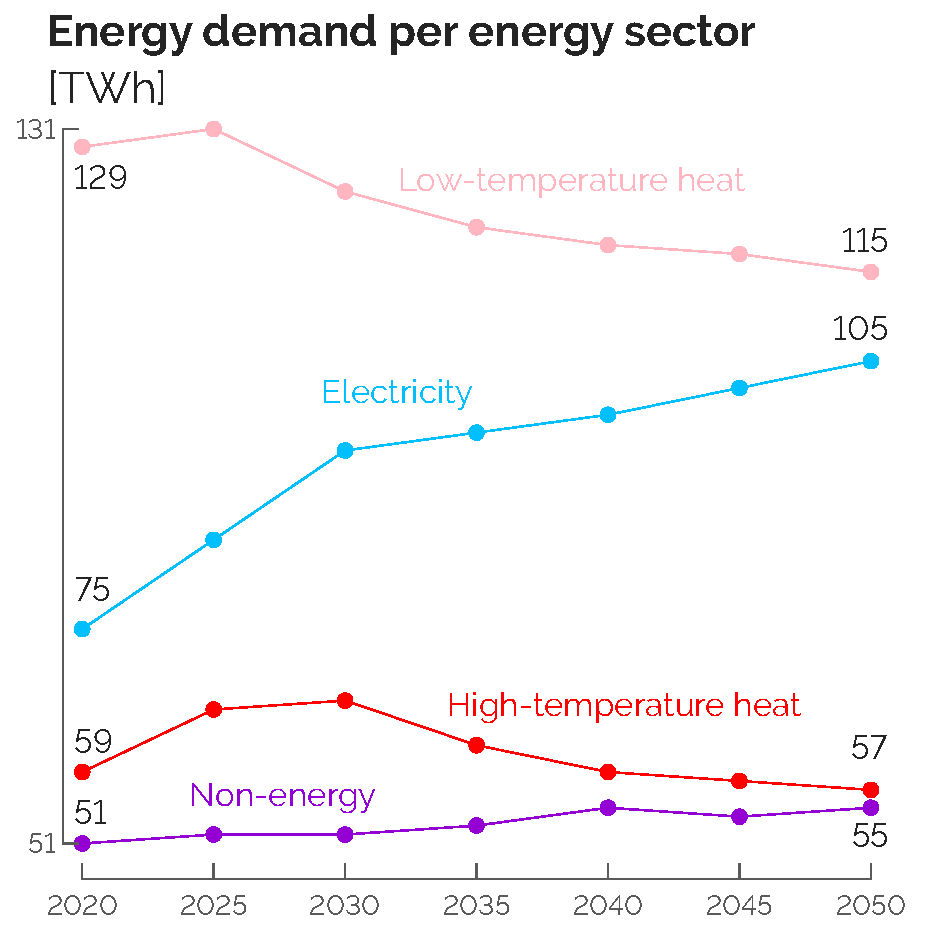
\includegraphics[width=0.43\textwidth]{EUD_sec.pdf}
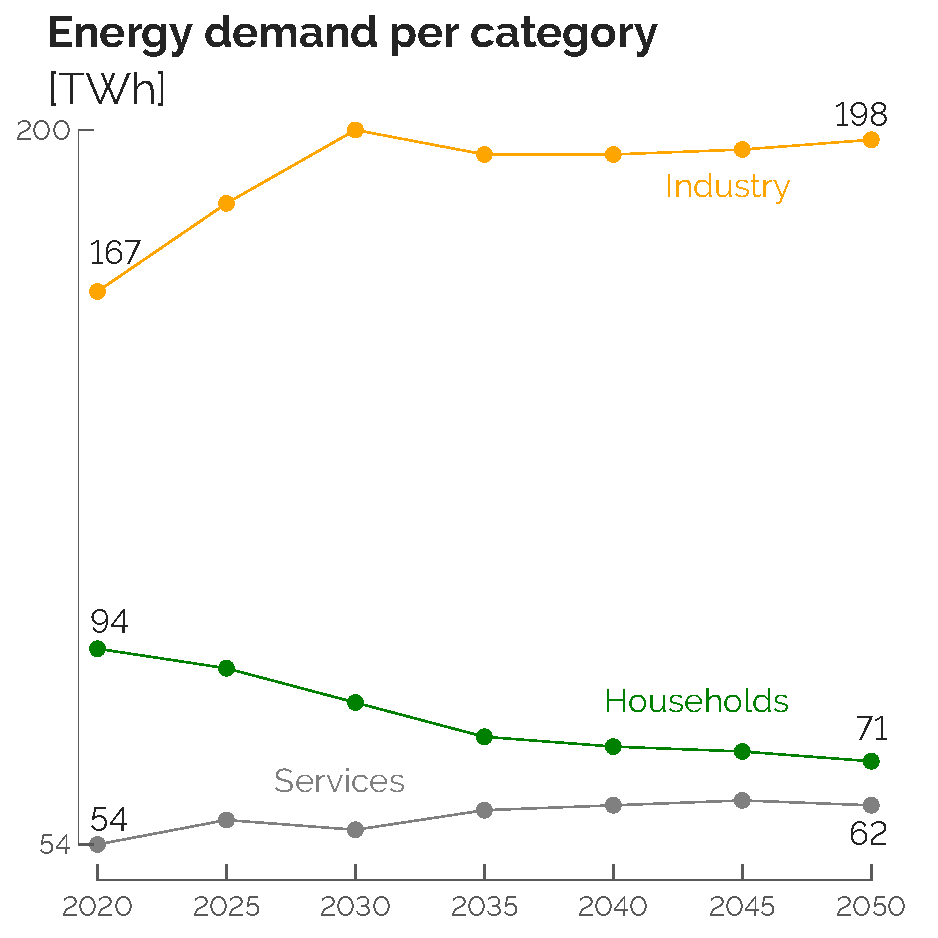
\includegraphics[width=0.43\textwidth]{EUD_cat.pdf}
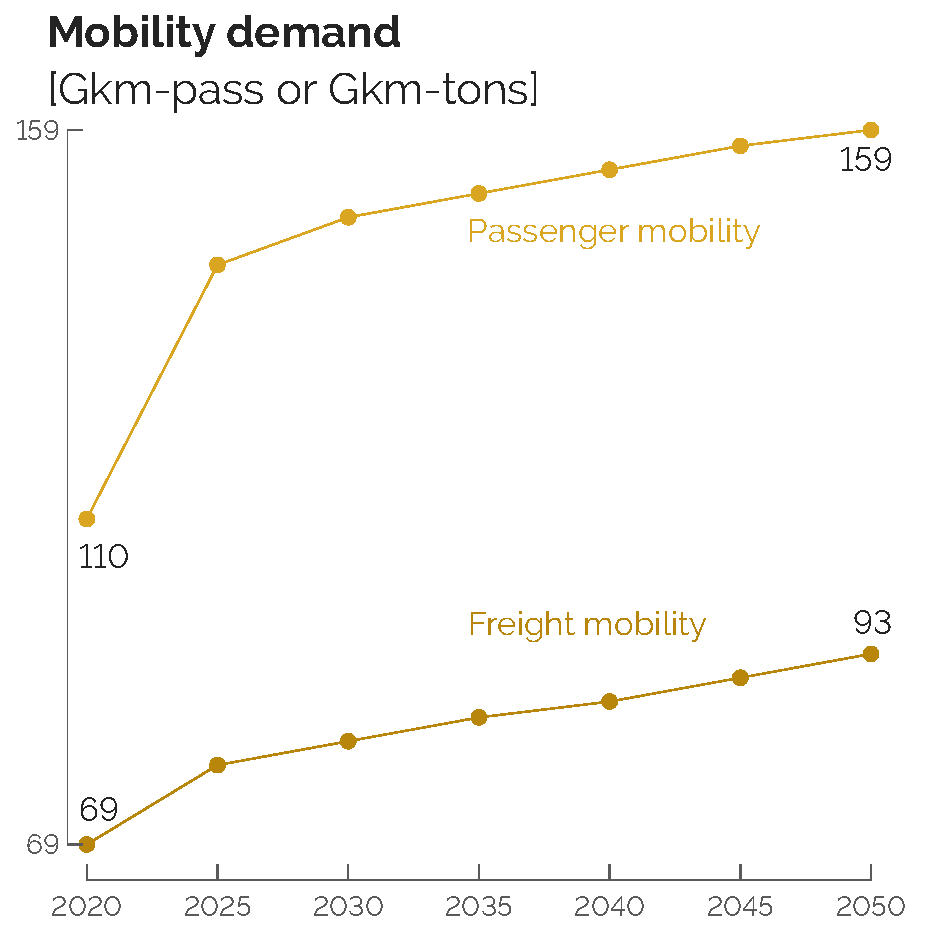
\includegraphics[width=0.43\textwidth]{EUD_mob.pdf}
\caption{EnergyScope splits the whole-energy system end-use demands (EUD) into two sets: (non)-energy and transport-related. This figure presents the yearly values of each of these demands. In the top-right graph, the non-energy demand has been fully associated with the industrial demand. This highlights the significant level of industrialisation of Belgium compared to the other sectors.}
\label{fig:cs_demands}
\end{figure}

To supply the aforementioned demands, EnergyScope Pathway implements a variety of resources defined by their cost of purchasing, $\mathit{c}_{\mathrm{op}}$ (see \Cref{fig:cs_resources_cost}), their availability, as well as their global warming potential, $\emph{gwp}_{\mathrm{op}}$, as detailed by \citet{limpens2024pathway}. Regarding the cost of ``renewable electrofuels'', they are in line with the recent study of \citet{genge2023supply} who carried out an extensive review and ``meta-analysis \cite{grant2009typology,page2021prisma} of 30 studies on the supply costs of chemical energy carriers''. 

\begin{figure}[htbp!]
\centering
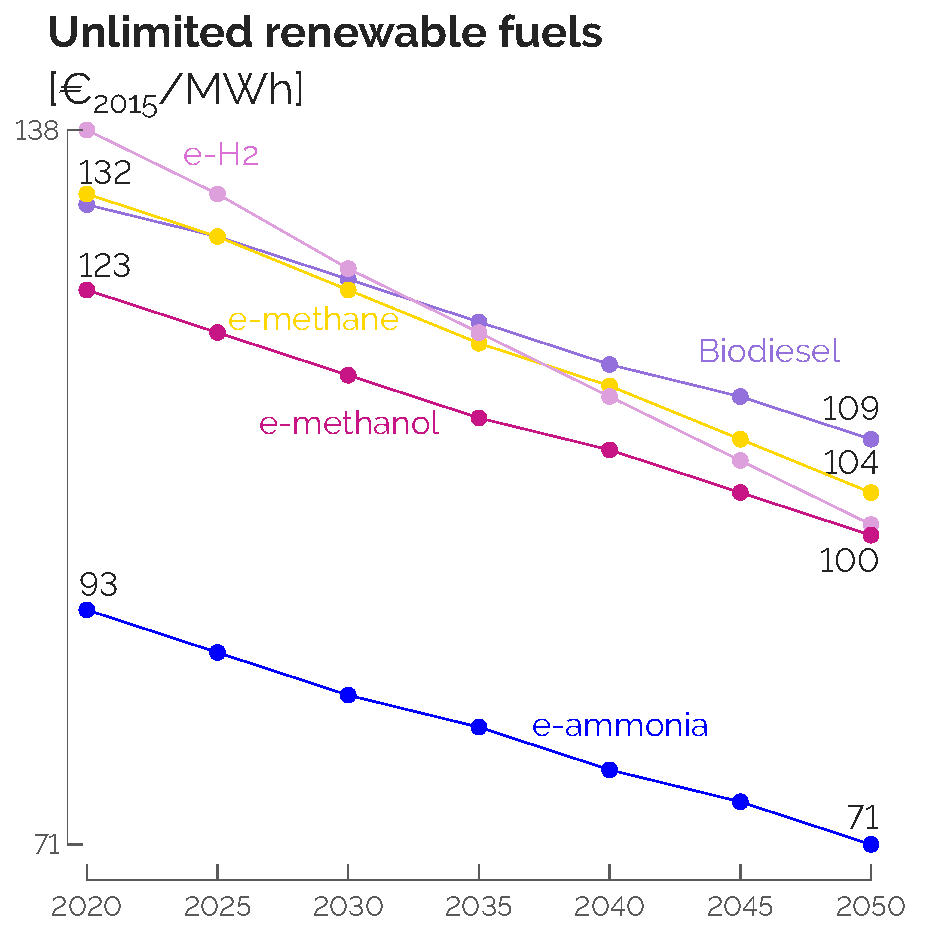
\includegraphics[width=0.43\textwidth]{Res_ren.pdf}
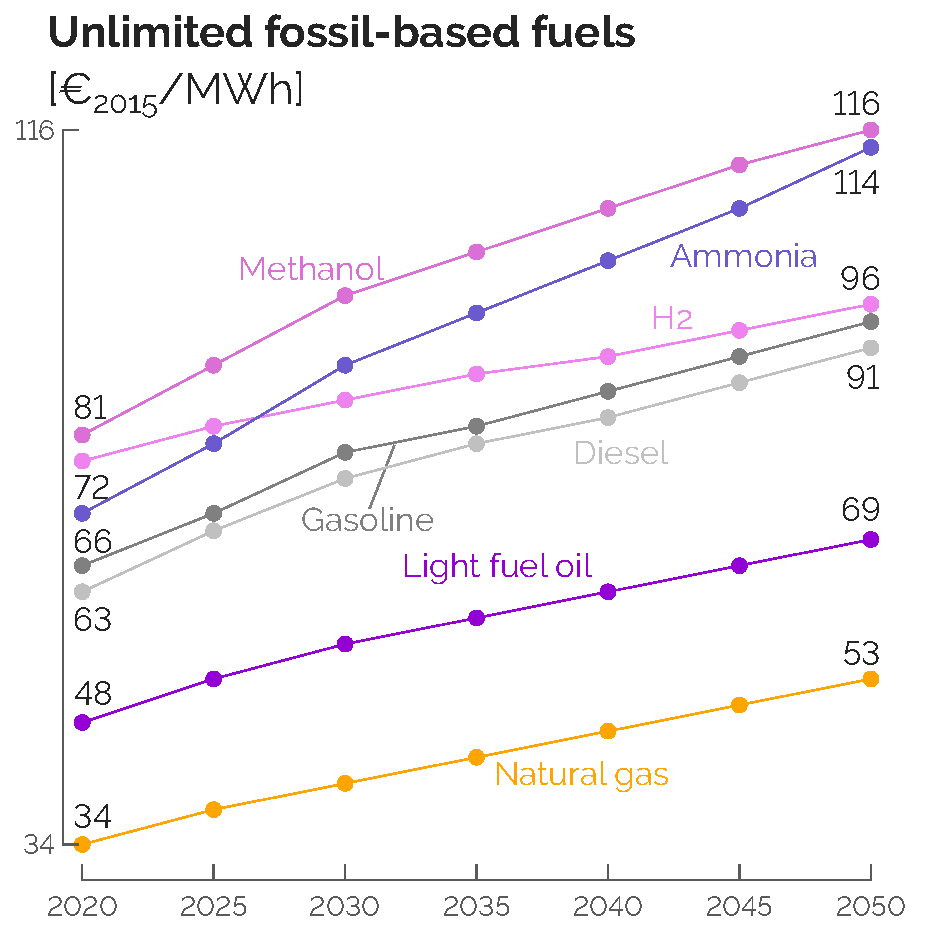
\includegraphics[width=0.43\textwidth]{Res_foss.pdf}
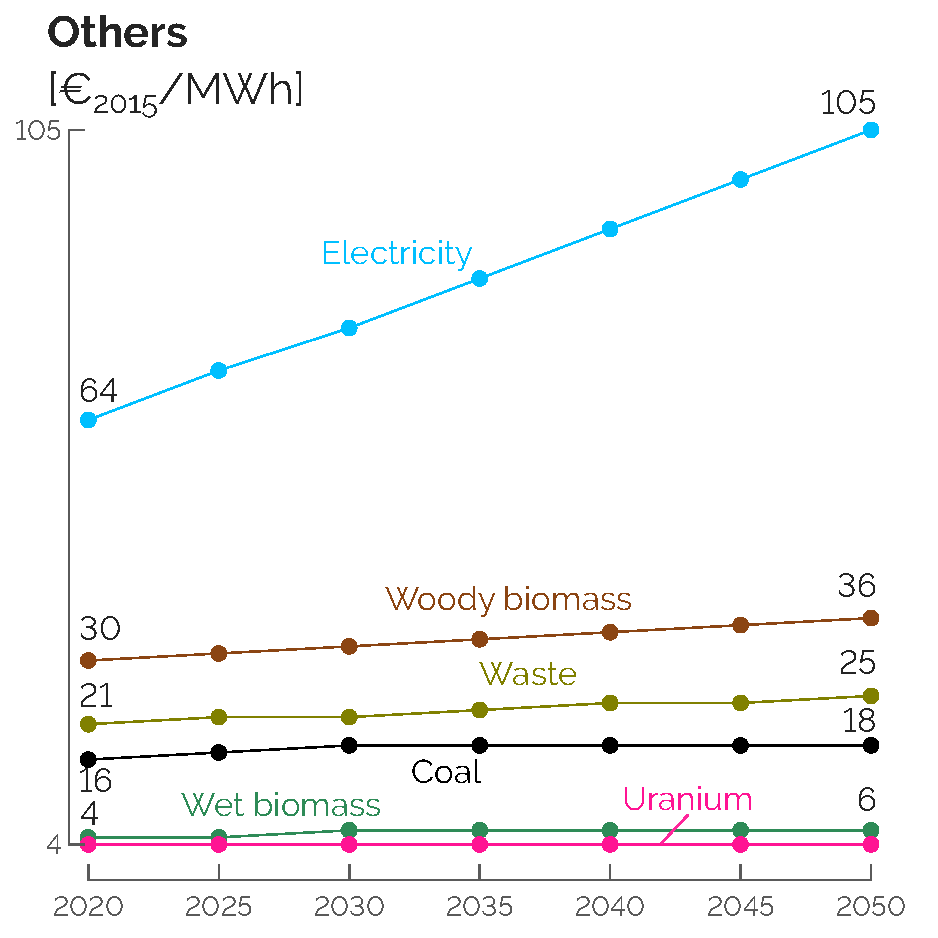
\includegraphics[width=0.43\textwidth]{Res_others.pdf}
\caption{Cost of purchasing the different resources. Besides the free local renewables (\ie sun, wind and hydro) limited by technical potentials, EnergyScope accounts for renewable energy carriers and their respective fossil counterparts (top-left and top-right). These fuels can be imported from abroad without limitation on their availability. Other carriers are limited either by their local potentials (\ie biomass and waste) or other considerations like the power grid interconnections or the capacity of nuclear power plants.}
\label{fig:cs_resources_cost}
\end{figure}

Regarding the imported renewable electrofuels, the \citet{h2coalition} has carried out an extensive techno-economic analysis to estimate their respective cost of purchasing, after having identified some key locations from which importing these energy carriers (\eg Chile, Australia or Morocco). As the amount to import from each of these locations is hard to forecast, the current work considers the average cost between the different locations. 

Besides the costs, the resources are either limited or unlimited in terms of availability and either renewable or not. The limitation in terms of availability can be direct or indirect. On the one hand, woody (23.4\,TWh) and wet biomass (38.9\,TWh) are directly limited by their local potentials and the consumption of waste (17.8\,TWh) and coal (33.4\,TWh) is assumed not to exceed the current use. Similarly to \citet{limpens2021generating}, we constrained the endogenous non-renewable wastes to be consumed locally. The local potential of biomass, \ie about 60\,TWh in total, could be considered as optimistic given the work of \citet{colla2024navigating} limiting this potential to about 40\,TWh. On the other hand, solar, wind, hydro and uranium are limited by the technical potentials of rooftop \gls{PV} panels (59.2\,GW), onshore (10\,GW) and offshore (6\,GW) wind turbines, run-of-the-river power plants (0.1\,GW) and the choice to limit nuclear power plants to 6\,GW, respectively. In line with the work of \citet{PATHS2050} and the maximum capacity of conventional nuclear reactors that have been installed in Belgium, the same 6\,GW are assumed to be the maximum capacity for \gls{SMR}. Imported electricity is limited in two ways: the potential of instantaneous capacity of interconnection with neighbouring countries (\ie 11.9\,GW by 2050 \cite{ELIA_2050}) and a limitation to 30\% of the yearly electricity end-use demand (\ie 32.4\,TWh by 2050) \cite{limpens2021generating}. 

Regarding the power grid interconnections with the neighbouring countries, similarly to the import of other energy carriers, there is no representation of those physical routes. The imported energy commodities are available ``at the front door'' of the system.  In terms of spatial resolution of the country itself, it is modelled as a single node. This is similar to the copper plate model of a power grid. In other words, the infrastructures to transport the energy carriers within the country are not considered.  It is assumed that the demands have to be supplied by the production, without considering the flows between the producers and the consumers. Yet, adapting the networks is accounted for in terms of the required investments. For instance, a high share of VRES requires an investment to reinforce the power grid (\ie 368\,M€/GW of additional installed capacity of \gls{VRES}). 

In the current work, imported electrofuels (\ie e-methane, e-hydrogen, e-methanol and e-ammonia) are assumed to be ``renewable'' in the sense that they do not increase the concentration of \ce{CO2} in the atmosphere \cite{rixhon2021terminology}. In practice, it means that their \gls{GWP} is assumed to be zero in the model. Compared to equivalent electrofuels that would be locally produced, this assumption does not account for the emissions related to the transport of imported electrofuels from abroad to Belgium. However, the share of these emissions is limited (between 5 and 10\%) compared to the whole cycle of production and use of imported electrofuels \cite{coppitters2024towards}. Therefore, the conclusions drawn in this thesis are not affected by this assumption. Besides these, every other resource has its specific \gls{GWP} like coal ($\emph{gwp}_{\mathrm{op,coal}}=0.40$\,kt$_{\ce{CO2},\text{eq}}$/GWh), natural gas ($\emph{gwp}_{\mathrm{op,NG}}=0.27$\,kt$_{\ce{CO2},\text{eq}}$/GWh) or the fossil-based molecules equivalent to the electrofuels (\eg $\emph{gwp}_{\mathrm{op,ammonia}}=0.46$\,kt$_{\ce{CO2},\text{eq}}$/GWh or $\emph{gwp}_{\mathrm{op,methanol}}=0.41$\,kt$_{\ce{CO2},\text{eq}}$/GWh).

As the end-use demands are defined as energy (and non-energy with the \gls{NED}) services rather than a certain quantity of oil or solar irradiance, for instance, technologies are implemented to convert these resources into end-use demands. Besides their CAPEX, OPEX and lifetime, production and conversion technologies (\ie \gls{CCGT}, car or boiler) have a conversion efficiency whereas storage technologies (\ie thermal storage, battery or molecule storage) have charge/discharge losses. There are also infrastructure technologies. They encompass, for instance, the power grid, the \gls{DHN} or technologies to produce intermediate energy carriers (\eg wood pyrolysis, biomethanolation or steam methane reforming to produce hydrogen). 

Not digging into too many more details about the exhaustive list of these technologies presented in previous work \cite{limpens2021generating}, this section rather focuses on the implementation of \gls{SMR} as the 6\,GW of conventional nuclear are assumed to drop to 2\,GW in 2025 and total phase-out by 2035. Similarly to the analysis of \citet{PATHS2050}, a Belgian consortium for energy research, and in line with the Belgian Nuclear Research Centre (SCK-CEN) \cite{SCK-CEN_SMR}, \gls{SMR} is implemented with the features listed in \Cref{tab:SMR_features}. Where most of the features are similar to conventional nuclear power plants, they differ from these on two main points: their potential year start, 2040, and their flexibility. Indeed, unlike the current nuclear power plants, constrained in the model to produce a constant power output at every hour of the year (\ie baseload production as it is actually the case in Belgium), SMRs, are flexible in the sense that their production can vary between 0 and their full capacity at any hour of each representative year. Here, we simplify SMRs as only producing electricity and we disregard the heat produced by the nuclear reaction. This is considered lost to the atmosphere.

\begin{table}[htbp!]
\caption{Nominal features of the SMRs in EnergyScope. \gls{SMR} exhibits the advantage to have a fully flexible production (\ie between 0 to the full capacity) unlike conventional nuclear that is constrained to produce a constant baseload at every hour of the year.}
\label{tab:SMR_features}
\begin{minipage}{\linewidth}
\centering
\begin{tabular}{l c c}
\toprule
\textbf{Feature} & \textbf{Value} & \textbf{Unit}\\
\midrule
CAPEX & 4850 & €/kW \\
Annual OPEX & 103\footnote{\label{foot:c_maint_SMR}This value is in line with \citet{smr_canada} that evaluate annual opex of 0.015\$/kWh, which makes 112\$/kW/year assuming a 85\% full-load availability, and \citet{PATHS2050} that accounts for 83.3€/kW/year} & €/kW/year \\
Lifetime & 60 & year \\
Cost of purchasing uranium & 4 & €/MWh\\
Efficiency & 40\% & -\\
Maximum capacity & 6 & GW \\
Annual availability & 85\%\footnote{\label{foot:avail_SMR}This annual availability accounts for yearly maintenance where the reactors might not operate or, at least, not at their maximum capacity. } & -\\
Operational year & 2040\footnote{\label{foot:op_year_SMR}2040 is the soonest year at which \gls{SMR} could be available, optimistically assuming industrial prototypes being completed by 2035 and 5 additional years for their commercial installation.} & - \\
Flexibility & Full & - \\
\bottomrule							

\end{tabular}
\end{minipage}
\end{table}

For the sake of comparison, the \gls{LCOE} of the principal technologies to produce electricity, based on the computation used by \citet{limpens2021generating}, is detailed (see \Cref{fig:LCOE}). Not included here is the cost of integrating a technology in the system (\eg reinforcement of the grid and storage capacities for \gls{VRES}), the \gls{LCOE} aims at aggregating and normalizing the CAPEX and OPEX of technologies providing a common commodity, \ie electricity. Compared to the other flexible generation units, \gls{SMR} is significantly more cost-effective. Besides being about six times more capital-intensive in €/kW, the investment is amortized over a longer expected lifetime (\ie 60 years). Moreover, the cost of purchasing uranium driving \gls{SMR} is expected to remain stable and low whereas the expected increase of the cost of purchasing fossil fuels dominates the \gls{LCOE} of \gls{CCGT}. In addition, one sees that \gls{CCGT} supplied by e-ammonia outcompetes its e-methane equivalent, unlike their respective fossil-based equivalent. This is because e-ammonia, not requiring carbon capture, is expected to be more cost-effective to produce versus e-methane \cite{h2coalition}. On the contrary, fossil-based ammonia, mostly relying on steam methane reforming, requires additional steps in the production process compared to fossil gas.

\begin{figure}[htbp!]
\centering
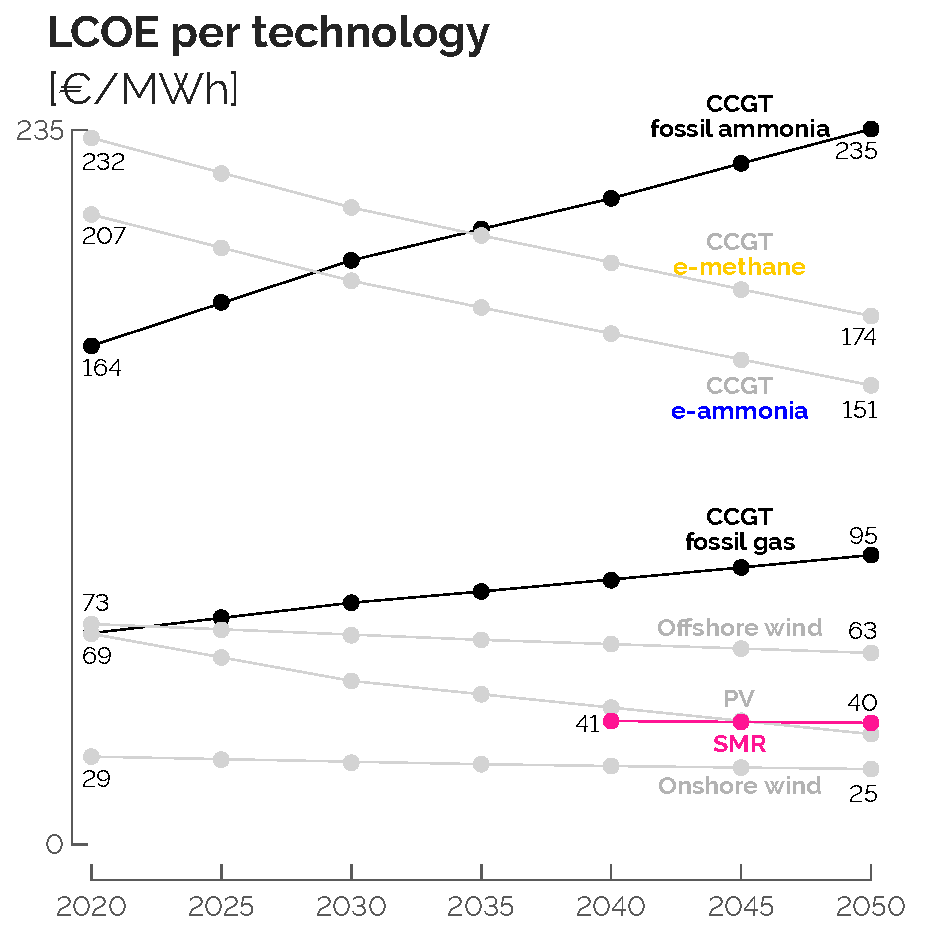
\includegraphics[width=0.49\textwidth]{LCOE_line_2.pdf}
\caption{Levelised cost of energy (LCOE) for the main technologies in the power sector. Grey and black curves are related to technologies running on renewable and fossil resources, respectively. \gls{SMR} is cheaper than the other flexible options. \gls{CCGT} running on e-ammonia is cheaper than its e-methane alternative.}
\label{fig:LCOE}
\end{figure}

\subsection{Uncertainty ranges}
\label{subsec:cs:uncertainty}
Accounting for uncertainty in \gls{ESOM} is crucial \cite{mavromatidis2018uncertainty}, especially when it comes to optimising several decades in an inherently uncertain future. The fundamental step in this ambition is to characterise these uncertainties.  Characterising precisely the uncertainty---ideally with their respective probability density functions (PDFs)---of the thousands of parameters in the model is daunting if not impossible because of lack of data \cite{marnay2006addressing}. Therefore, we used a workaround developed by \citet{Moret2017} that defines relative ranges of variation for different groups of parameters. These ranges have been adapted for the Belgian energy system and the pathway formulation.  For the operation-type parameters (types II and III), a scaling factor needs to be considered to avoid assuming that the uncertainty for the last year of the planning horizon ($N$) is representative for all years in the planning horizon \citet{Moret2017}. In EnergyScope Pathway, as the model optimises the system every 5 years, $N=5$ has been selected to get the final ranges of uncertainties of type II and III. For type III uncertainties (\ie uncertainty ranges increasing with time), a 50\% increase has been set arbitrarily between the ranges for 2025 and these same ranges for 2050. In other words, for these specific uncertainties, the ranges for 2050 are 50\% larger than for 2025. Like other works \cite{li2019renewables,coppitters2021robust}, the uncertain parameters are assumed to be independent and uniformly distributed between their respective lower and upper bounds. 

\citet{rixhon2021role} analysed the impact of these parameters on the total cost of the snapshot Belgian whole-energy system in 2050 subject to different \gls{GWP} limits. Based on this work, we have selected a subset of impacting uncertainties, added others due to the pathway formulation (\eg $\Delta_{\mathrm{change,pass}}$), and listed them in Table \ref{tab:UC_full} that summarises the uncertainty ranges for the different groups of technologies and resources, for the year 2025.  Moreover, some ranges have been added to account for new parameters coming from the pathway formulation described in {\color{red} \Cref{subsec:meth:ES_Pathway}} like the society inertia (\eg $\Delta_{\mathrm{change,pass}}$). 

A particular attention is to pay to the potential installation of \gls{SMR}. As detailed in \Cref{app:dem_res_tech}, the commercial availability of such a technology is uncertain but would not be before 2040. Consequently, for \gls{SMR}, the parameter $f_{\mathrm{max,SMR}}$ influences the maximum capacity to install to translate somehow the readiness of this technology. As SMRs are foreseen, if installed, to be around the same locations (\ie Tihange and Doel) as the conventional nuclear power plants and using the same area in kW/ha, the same 6\,GW are assumed to be the maximum capacity for SMRs. If it is (i) smaller than 0.6, there is no possibility to install \gls{SMR} during the transition; (ii) between 0.6 and 0.8, these 6~GW can be installed only in 2050; (iii) between 0.8 and 0.9, these can be installed from 2045 onward and; (iv) higher than 0.9, the prescribed maximum capacity can be installed from 2040 onward. Based on the local sensitivity analysis carried out by \citet{PATHS2050}, the current work also considers a [-40\%; +44\%] range on the CAPEX of SMR, on top of the uncertainty about the availability. Finally, the the cost of purchasing renewable electrofuels presents a wide range, [-64.3\%; +179.8\%], like the other imported commodities.

\begin{table}[htbp!]
\caption{Application of the uncertainty characterization method of \citet{Moret2017PhDThesis} to the EnergyScope Pathway model for the year 2025. }
\label{tab:UC_full}
\begin{minipage}{\linewidth}
\centering
\resizebox{\textwidth}{!}{
\begin{tabular}{l l l c c c}
\toprule
\multirow{2}{*}{\textbf{Category}} & \multirow{2}{*}{\textbf{Parameter}} & \multirow{2}{*}{\textbf{Meaning}} & \multirow{2}{*}{\textbf{Type}\footnote{\label{foot:type_uncert_range_app}Per \citet{Moret2017PhDThesis}, \og I: investment-type, II: operation-type (constant uncertainty over time), III: operation-type (uncertainty increasing over time)\fg . }}  & \multicolumn{2}{c}{\textbf{Relative variation}\footnote{\label{foot:nom_val_uncert_app}The nominal values of each of the parameters is 0, meaning no variation compared to the nominal values of the impacted parameter in the model. }}\\
    & & & &	 min 	&	 max \\ 	
\midrule		
\multirow{4}{*}{\textbf{Cost of purchasing}} & $c_{\mathrm{op,fossil}}$ & Purchase fossil fuels & II & -64.3\% & 179.8\% \\
& $c_{\mathrm{op,elec}}$ & Purchase electricity & II & -64.3\% & 179.8\% \\
& $\mathbf{c_{\mathrm{op,electrofuels}}}$ & \textbf{Purchase electrofuels} & \textbf{II} & \textbf{-64.3\%} & \textbf{179.8\%} \\
& $c_{\mathrm{op,biofuels}}$ & Purchase biofuels & II & -64.3\% & 179.8\% \\
\midrule
\multirow{9}{*}{\textbf{Investment cost}} &$c_{\mathrm{inv,car}}$ & CAPEX car  & I & -21.6\% & 25.0\% \\
& $c_{\mathrm{inv,bus}}$ & CAPEX bus & I & -21.6\% & 25.0\% \\
& $c_{\mathrm{inv,ic\_prop}}$ & CAPEX ICE & I & -21.6\% & 25.0\% \\
& $c_{\mathrm{inv,e\_prop}}$ & CAPEX electric motor & I & -39.6\% & 39.6\% \\
& $c_{\mathrm{inv,fc\_prop}}$ & CAPEX fuel cell engine & I & -39.6\% & 39.6\% \\
& $c_{\mathrm{inv,efficiency}}$ & CAPEX efficiency measures & I & -39.3\%  & 39.3\% \\
& $c_{\mathrm{inv,PV}}$ & CAPEX PV & I & -39.6\% & 39.6\% \\
& $c_{\mathrm{inv,grid}}$ & CAPEX power grid & I & -39.3\% & 39.3\% \\
& $c_{\mathrm{inv,grid\_enforce}}$ & CAPEX grid reinforcement & I & -39.3\% & 39.3\% \\
& $\mathbf{c_{\mathrm{inv,nuclear\_SMR}}}$ & \textbf{CAPEX \gls{SMR}}\footnote{\label{foot:range_SMR_app}This range has been inferred from the local sensitivity analysis performed by \citet{PATHS2050}.} & \textbf{I} & \textbf{-40.0\%} & \textbf{44.0\%} \\
\midrule
\textbf{Maintenance cost} & $c_{\mathrm{maint,var}}$ & Variable OPEX of technologies & I & -48.2\% & 35.7\% \\
\midrule
\multirow{2}{*}{\textbf{Consumption}} &$\eta_{\mathrm{e\_prop}}$ & Consumption electric vehicles & I & -28.7\% & 28.7\% \\
& $\eta_{\mathrm{fc\_prop}}$ & Consumption fuel cell vehicles & I & -28.7\% & 28.7\% \\
\midrule
\multirow{3}{*}{\textbf{Potential installed capacity}} &$f_{\mathrm{max,PV}}$ & Max capacity PV & I & -24.1\% & 24.1\% \\
& $f_{\mathrm{max,windon}}$ & Max capacity onshore wind & I & -24.1\% & 24.1\% \\
& $f_{\mathrm{max,windoff}}$ & Max capacity offshore wind & I & -24.1\% & 24.1\% \\
& $\mathbf{f_{\mathrm{max,SMR}}}$ & \textbf{Potential capacity \gls{SMR}} & \textbf{-} & \textbf{0} & \textbf{1} \\
\midrule
\multirow{2}{*}{\textbf{Hourly load factor}} & $c_{\mathrm{p,t,PV}}$ & Hourly load factor PV & II & -22.1\% & 22.1\% \\
& $c_{\mathrm{p,t,winds}}$ & Hourly load factor wind turbines & II & -22.1\% & 22.1\% \\
\midrule
\multirow{2}{*}{\textbf{Resource availability}} & $avail_{\mathrm{elec}}$ & Available electricity import & I & -32.1\% & 32.1\% \\
& $avail_{\mathrm{biomass}}$ & Available local biomass & I & -32.1\% & 32.1\% \\
\midrule

\multirow{4}{*}{\textbf{End-use demand}} &$HH\_EUD$ & Households EUD & III & -13.8\% & 11.2\% \\
& $services\_EUD$ & Services EUD & III & -14.3\% & 11\% \\
& $pass\_EUD$ & Passenger mobility EUD & III & -7.5\% & 7.5\% \\
& $industry\_EUD$ & Industry EUD & III & -20.5\% & 16.0\% \\
\midrule

\multirow{5}{*}{\textbf{Miscellaneous}} &$i_{\mathrm{rate}}$  & Discount rate & I & -46.2\% & 46.2\% \\
& $\%_{\mathrm{pub,max}}$ & Max share of public transport & I & -10\% & 10\% \\
& $\Delta_{\mathrm{change,freight}}$ & Modal share change freight mobility & - & -30\% & 30\% \\
& $\Delta_{\mathrm{change,pass}}$ & Modal share change passenger mobility & - & -30\% & 30\% \\
& $\Delta_{\mathrm{change,LT\_heat}}$ & Modal share change LT-heat & - & -30\% & 30\% \\
\bottomrule							

\end{tabular}}
\end{minipage}
\end{table}

This work considers nine groups of uncertain parameters: (i) the cost of purchasing imported energy carriers; (ii) the investment cost (\ie CAPEX) of some technologies, mostly related to the mobility sector and the integration of renewables; (iii) the maintenance cost (\ie OPEX) of every technology; (iv) the consumption of electric and fuel cells vehicles in the mobility sector; (v) the potential installed capacity of renewables; (vi) the hourly load factor of renewables accounting for the variability of solar irradiance or wind speed; (vii) the availability of resources considered limited (\ie biomass and electricity); (viii) the end-use-demands split per sector of activities (\ie households, services, passenger mobility and industry) and (ix) other parameters like the discount rate or the exogenous modal share change in different key sectors. A particular attention is to pay to the potential installation of \gls{SMR}, at the bottom of \Cref{tab:UC_full}. As detailed before, the commercial availability of such a technology is uncertain but would not be before 2040. Consequently, for \gls{SMR}, the parameter $f_{\mathrm{max,SMR}}$ influences the maximum capacity to install to translate somehow the readiness of this technology. Arbitrarily, we have then assumed the following probability of availability of such a technology: 10\% chance to be installable from 2040, 20\% from 2045 and 40\% from 2050\footnote{In other words, if this parameter, ranging between 0 and 1, is (i) smaller than 0.6, there is no possibility to install \gls{SMR} during the transition; (ii) between 0.6 and 0.8, these 6~GW can be installed only in 2050; (iii) between 0.8 and 0.9, these can be installed from 2045 onward and; (iv) higher than 0.9, the prescribed maximum capacity can be installed from 2040 onward. }. Based on the local sensitivity analysis carried out by \citet{PATHS2050}, the current work also considers a [-40\%; +44\%] range on the CAPEX of SMR, on top of the uncertainty about its availability. Finally, the cost of purchasing renewable electrofuels presents a wide range, [-64.3\%; +179.8\%], like the other imported commodities.

\subsection{\ce{CO2} budget for the transition}
\label{subsec:cs:CO2-budget}
In most studies carried out on the pathway optimisation of a whole-energy system, a \ce{CO2}-trajectory is \textit{a priori} set to reach carbon neutrality by 2050. \citet{nerini2017myopic} used the emission trajectory indicated by the UK's Committee on Climate Change in their analysis of the impact of limited foresight to achieve the target of 80\% reduction of \gls{GHG} by 2050 in the United Kingdom. In their assessment of the impacts of economy-wide emission policies in the water-energy-land nexus, \citet{licandeo2023assessing} analysed different \ce{CO2} trajectories considering more or less severe water scarcity for the US. \citet{poncelet2016myopic} with LUSYM (Leuven University SYstem Model) and \citet{PATHS2050} with TIMES-BE also set decreasing emission trajectories in their analysis of respectively the Belgian power sector and whole-energy system.  Others only set the objective of carbon neutrality by 2050. For instance, \citet{heuberger2018impact} investigated the impact of different factors (\eg limit of the foresight in the future, availability of \og unicorn technologies\fg or committed versus market-driven decarbonisation strategies) to reach this ultimate objective in the UK system. In their ``near-term to net zero'' (NT2NZ) approach to estimate \ce{CO2} prices, \citet{kaufman2020near} emphasises the need to select, \textit{a priori}, an emissions pathway to the net-zero target. Some authors suggest limiting near-term technological disruptions and, consequently, the initial rate of emission reductions \cite{wigley1996economic} whereas others, to avoid technology lock-in and to benefit from early investments in the transition, encourage a sharper decrease of the emissions at an earlier stage \cite{vogt2018starting}.

In this work, the effect of greenhouse gases is cumulative over time and a constraint is set on the overall emissions of the transition---a \ce{CO2} budget for the transition. This approach is in line with the works defining safe operating spaces within the nine different global planetary boundaries (\ie (i) novel entities, (ii) stratospheric ozone depletion, (iii) atmospheric aerosol loading, (iv) ocean acidification, (v) biogeochemical flows, (vi) freshwater change, (vii) land system change, (viii) biosphere integrity, and, (ix) climate change) \cite{richardson2023earth,steffen2015planetary,rockstrom2009safe}. This ``systemic framework for addressing global anthropogenic impacts on Earth system'' gives quantitative recommendations about the \ce{CO2} concentration, among others, to maintain ``the stability and resilience of Earth system as a whole'' \cite{richardson2023earth}. In their review, \citet{ryberg2020downscaling} identified three main sharing principle categories when considering these safe spaces: \ie \textit{utilitarian}, \textit{egalitarian} and \textit{acquired rights} principles. In a nutshell, the former, mostly applied to the industry sector \cite{ryberg2018bring,brejnrod2017absolute}, aims at maximising the sum of welfare. The second shares the so-called ``budget'' equally among the total population, allocating the same share to each individual \cite{hoff2017bringing,o2018good}. Finally, in \textit{acquired rights} principles, also called ``grandfathering'', the sharing is based on \og maintaining that prior emissions increase future emission entitlements\fg  \cite{knight2013grandfathering}. In this thesis, we have chosen the latter principle to allocate the \ce{CO2} budget to the Belgian transition. This budget (1.2\,Gt$_{\ce{CO2},\text{eq}}$) corresponds to the proportion of Belgium's emissions in the world energy-related emissions in 2020 (34.8\,Gt$_{\ce{CO2},\text{eq}}$ \cite{ourworldindata_CO2_world}) applied to the global budget to have a 66\% chance of limiting warming to 1.5°C of 420\,Gt$_{\ce{CO2},\text{eq}}$ \cite{IPCC_CO2_budget}. Therefore, in this work, a limit has been put on $\emph{gwp\textsubscript{lim,trans}}=1.2\,\text{Gt}_{\ce{CO2},\text{eq}}$ in Equation\,(\ref{eq:limit_gwp_trans}). This is another sign of the urgency to act to mitigate climate change as this 30-year budget represents only 10 years of the current emissions.  In this approach, the residual emissions in 2050 are not explicitly constrained down to zero. This carbon neutrality is rather implicit given the ambitious \ce{CO2} budget.

\section{Supplementary results of the uncertainty quantification}

\subsection{Total transition cost}
\label{app:UQ_transition_cost}

\Cref{tab:UQ_full} gives the ranking and total Sobol index over the total transition cost of each of the 34 parameters listed in \Cref{tab:UC_full}. The first column shows these indicators for the \gls{GSA} applied on the hourly pathway model. For information, the second column gives the same indicators but for an uncertainty quantification carried out on the monthly pathway model that has some limitations \cite{limpens2024pathway} but has the main advantage of running much faster. Given the similar rankings of the parameters between these two, this comparison shows that the monthly model can be a computationally efficient proxy to quantify the uncertainties of the actual hourly model and point out the key parameters of the optimisation-driving objective, the total transition cost. 

Besides the top-4 parameters, rankings are slightly different. The main difference in terms of ranking relates to the import of electricity from abroad, \ie its cost of purchasing and its availability. Indeed, as observed by \citet{limpens2024pathway}, the monthly model does not require this import given the easier integration of monthly-averaged local \gls{VRES}. However, this does not jeopardize the comparative analysis given the similar Sobol' indices. Given their wide range of uncertainty [-64.3\%; 179.8\%] and their significant role in meeting the \ce{CO2} budget, the cost of purchasing electrofuels is the first, by far, impacting parameter. Next, comes, naturally, the industrial \gls{EUD}, representing, at the nominal value, 60\% of the total demands by 2050. The top 3 are completed by the variation of the discount rate, directly impacting the annualisation and the salvage values of the assets. Finally, since the current Belgian whole-energy system deeply relies on fossil resources, and would still do so in the near future, the cost of purchasing fossil fuels is part of the impacting parameters. On the contrary, due to the very low annualised, cost, and long lifetime leading to a significant salvage value and a low-emitting fuel, the parameters related to \gls{SMR} barely impact the total transition cost.


\begin{table}[htbp!]
\caption{Total Sobol' indices of the uncertain parameters over the total transition cost.}
\label{tab:UQ_full}
\begin{minipage}{\textwidth}
\centering
\resizebox{0.8\textwidth}{!}{
\begin{tabular}{l c c}
\toprule
\textbf{Parameter}  & \multicolumn{2}{c}{\textbf{Ranking (Sobol' index)}}\\
\midrule
\textbf{Purchase electrofuels} & 1 & (46.8\%) \\
Industry EUD & 2 & (23.2\%) \\
Discount rate & 3 & (12.0\%) \\
Purchase fossil fuels & 4 & (5.7\%) \\
\midrule
Variable OPEX of technologies & 5 & (3.1\%) \\
Purchase biofuels & 6 & (2.6\%) \\
CAPEX electric motor & 7 & (2.1\%) \\
Purchase electricity & 8 & (1.5\%) \\
Hourly load factor wind turbines & 9 & (1.1\%) \\
Hourly load factor PV & 10 & (1.1\%) \\
\textbf{Potential capacity \gls{SMR}} & 11 & (0.9\%) \\
CAPEX car & 12 & (0.8\%) \\
Available local biomass & 13 & (0.7\%) \\
Passenger mobility EUD & 14 & (0.7\%) \\
Modal share change LT-heat & 15 & (0.5\%) \\
Max capacity PV & 16 & (0.5\%) \\
Households EUD & 17 & (0.5\%)\\
Services EUD & 18 & (0.5\%) \\
Max share of public transport & 19 & (0.3\%) \\
Max capacity onshore wind & 20 & (0.3\%) \\
CAPEX PV & 21 & (0.2\%) \\
Efficiency electric motor & 22 & (0.2\%) \\
Max capacity offshore wind & 23 & (0.2\%) \\
Available electricity import & 24 & (0.1\%) \\
CAPEX ICE & 25 & (0.1\%) \\
CAPEX fuel cell engine & 26 & (0.1\%) \\
Efficiency fuel cell engine & 27 & (0.1\%) \\
Modal share change freight mobility & 28 & (0.1\%) \\
Modal share change passenger mobility & 29 & ($<$0.1\%) \\
CAPEX grid reinforcement & 30 & ($<$0.1\%) \\
CAPEX efficiency measures & 31 & ($<$0.1\%)\\
CAPEX bus & 32 &($<$0.1\%)  \\
\textbf{CAPEX \gls{SMR}} & 33 & ($<$0.1\%) \\
CAPEX power grid & 34 & ($<$0.1\%)\\
\bottomrule							

\end{tabular}}
\end{minipage}
\end{table}





%\begin{table}[htbp!]
%\caption{Total Sobol' indices of the uncertain parameters over the total transition cost in the monthly and hourly pathway models. The similar rankings (and indices) show the validity of using the faster (even though less accurate) monthly model to assess uncertainties over the hourly model.}
%\label{tab:UQ_full}
%\centering
%\begin{tabular}{l c c|c c| c c}
%\toprule
%\multirow{2}{*}{\textbf{Parameter}}  & \multicolumn{6}{c}{\textbf{Ranking (Sobol' index)}}\\
%& \multicolumn{2}{c}{Hourly model} & \multicolumn{2}{c|}{Monthly model} 	& \multicolumn{2}{c}{Hourly model} \\ 	
%\midrule
%\textbf{Purchase electrofuels} & 1 & (46.8\%) & 1 & (47.4\%) & 1 & (44.4\%) \\
%Industry EUD & 2 & (23.2\%) & 2 & (23.5\%) & 2 & (26.4\%)  \\
%Discount rate & 3 & (12.0\%) & 3 & (11.0\%) &  3 & (13.2\%)  \\
%Purchase fossil fuels & 4 & (5.7\%) & 4 & (6.9\%) & 4 & (6.9\%)   \\
%\midrule
%Variable OPEX of technologies & 5 & (3.1\%) & 5 & (2.9\%) & 6 & (3.0\%) \\
%Purchase biofuels & 6 & (2.6\%) & 6 & (2.6\%) & 5 & (3.0\%) \\
%CAPEX electric motor & 7 & (2.1\%) & 8 & (1.9\%) & 7 & (2.5\%) \\
%Purchase electricity & 8 & (1.5\%) & 34 & ($<$0.1\%) & \multicolumn{2}{c}{-} \\
%Hourly load factor wind turbines & 9 & (1.1\%) & 9 & (1.3\%) & 8 & (1.4\%) \\
%Hourly load factor PV & 10 & (1.1\%) & 7 & (1.9\%) & 9 & (1.3\%) \\
%\textbf{Potential capacity \gls{SMR}} & 11 & (0.9\%) & 11 & (0.9\%) & 11 & (1.0\%) \\
%CAPEX car & 12 & (0.8\%) & 13 & (0.7\%) & 10 & (1.2\%) \\
%Available local biomass & 13 & (0.7\%) & 12 & (0.8\%) & 12 & (0.7\%) \\
%Passenger mobility EUD & 14 & (0.7\%) & 14 & (0.7\%) & 13 & (0.7\%) \\
%Modal share change LT-heat & 15 & (0.5\%) & 15 & (0.5\%) & \multicolumn{2}{c}{-} \\
%Max capacity PV & 16 & (0.5\%) & 10 & (1.1\%) & 14 & (0.5\%) \\
%Households EUD & 17 & (0.5\%) & 16 & (0.5\%) & \multicolumn{2}{c}{-} \\
%Services EUD & 18 & (0.5\%) &  17 & (0.4\%) & \multicolumn{2}{c}{-} \\
%Max share of public transport & 19 & (0.3\%) & 19 & (0.3\%) & \multicolumn{2}{c}{-} \\
%Max capacity onshore wind & 20 & (0.3\%) & 18 & (0.3\%) & \multicolumn{2}{c}{-} \\
%CAPEX PV & 21 & (0.2\%) & 20 & (0.2\%) & \multicolumn{2}{c}{-} \\
%Efficiency electric motor & 22 & (0.2\%) & 22 & (0.1\%) & \multicolumn{2}{c}{-} \\
%Max capacity offshore wind & 23 & (0.2\%) & 21 & (0.2\%) & \multicolumn{2}{c}{-} \\
%Available electricity import & 24 & (0.1\%) & 33 & ($<$0.1\%) & \multicolumn{2}{c}{-} \\
%CAPEX ICE & 25 & (0.1\%) & 24 & (0.1\%) & \multicolumn{2}{c}{-} \\
%CAPEX fuel cell engine & 26 & (0.1\%) & 23 & (0.1\%) & \multicolumn{2}{c}{-} \\
%Efficiency fuel cell engine & 27 & (0.1\%) & 25 & ($<$0.1\%) & \multicolumn{2}{c}{-} \\
%Modal share change freight mobility & 28 & (0.1\%) & 26 & ($<$0.1\%) & \multicolumn{2}{c}{-} \\
%Modal share change passenger mobility & 29 & ($<$0.1\%) & 27 & ($<$0.1\%) & \multicolumn{2}{c}{-} \\
%CAPEX grid reinforcement & 30 & ($<$0.1\%) & 30 & ($<$0.1\%) & \multicolumn{2}{c}{-} \\
%CAPEX efficiency measures & 31 & ($<$0.1\%) & 28 & ($<$0.1\%) & \multicolumn{2}{c}{-} \\
%CAPEX bus & 32 &($<$0.1\%)  & 29 & ($<$0.1\%) & \multicolumn{2}{c}{-} \\
%\textbf{CAPEX \gls{SMR}} & 33 & ($<$0.1\%)  & 32 & ($<$0.1\%) & \multicolumn{2}{c}{-} \\
%CAPEX power grid & 34 & ($<$0.1\%) & 31 &  & \multicolumn{2}{c}{-} \\
%\bottomrule							
%
%\end{tabular}
%\end{table}

\newpage
\subsection{Imported renewable electrofuels}
\label{app:UQ_electrofuels}
\begin{table}[htbp!]
\caption{Comparison of the quantities of imported renewable electrofuels, in TWh, between the REF case, the SMR case and the statistical features from the \gls{GSA} (\ie Q1, median and Q3). 2020 is not in the table as, per assumption, no renewable electrofuel is imported for this year. For the sake of clarity, zeroes are replaced by ``-''.}
\label{tab:uq_ref_smr_med}
\begin{minipage}{\textwidth}
\centering
\resizebox{0.8\textwidth}{!}{
\begin{tabular}{l l | c c c c}
\toprule
\textbf{Year} & \textbf{Case} & \textbf{e-methane} & \textbf{e-hydrogen} & \textbf{e-ammonia} & \textbf{e-methanol}\\	
\toprule							
\multirow{5}{*}{2025}
 & REF & - & - & 10 & 52\\
 & SMR & - & -  & 10 & 29\\
 \cmidrule{2 - 6}
 & Q1 & - & - & 9 & 2\\
 & Median & - & - & 10 & 47\\
 & Q3 & - & - & 11 & 55\\
\toprule
\multirow{5}{*}{2030}
 & REF & - & 1 & 10 & 52\\
 & SMR & - & 1 & 10 & 52\\
 \cmidrule{2 - 6}
 & Q1 & - & - & 9 & 43\\
 & Median & - & - & 10 & 50\\
 & Q3 & - & 1 & 12 & 57\\
\toprule
\multirow{5}{*}{2035}
 & REF & - & 17 & 10 & 53\\
 & SMR & - & 17 & 10 & 53\\
 \cmidrule{2 - 6}
 & Q1 & - & - & 9 & 42\\
 & Median & - & 5 & 11 & 51\\
 & Q3 & - & 16 & 33 & 58\\
\toprule
\multirow{5}{*}{2040}
 & REF & - & 16 & 23 & 54\\
 & SMR & - & 16 & 10 & 54\\
 \cmidrule{2 - 6}
 & Q1 & - & - & 10 & 41\\
 & Median & - & 12 & 26 & 51\\
 & Q3 & 8 & 16 & 68 & 60\\
\toprule
\multirow{5}{*}{2045}
 & REF & 40 & 16 & 42 & 54\\
 & SMR & - & 16 & 11 & 54\\
 \cmidrule{2 - 6}
 & Q1 & - & - & 12 & 42\\
 & Median & - & 12 & 37 & 52\\
 & Q3 & 35 & 17 & 71 & 60\\
\toprule
\multirow{5}{*}{2050}
 & REF & 39 & 16 & 44 & 55\\
 & SMR & 7 & 16 & 11 & 55\\
 \cmidrule{2 - 6}
 & Q1 & - & - & 11 & 43\\
 & Median & 1 & 13 & 31 & 53\\
 & Q3 & 36 & 17 & 66 & 61\\
\bottomrule							
\end{tabular}}
\end{minipage}
\end{table}

Figures \ref{fig:results_uq_prod_cons_Gas}, \ref{fig:results_uq_prod_cons_H2}, \ref{fig:results_uq_prod_cons_Ammonia} and \ref{fig:results_uq_prod_cons_Methanol} give the distribution of the different routes of supply and consumption of methane, hydrogen, ammonia and methanol, resulting from the 1260 samples of the \gls{GSA}.

Given its lower cost of purchasing than its renewable equivalent (\Cref{fig:cs_resources_cost}) and lower \gls{GWP} than other fossil fuels (\ie $\mathit{gwp}_{\mathrm{op,NG}}=0.27$\,kt$_{\ce{CO2},\text{eq}}$/GWh versus $\mathit{gwp}_{\mathrm{op,LFO}}=0.31$\,kt$_{\ce{CO2},\text{eq}}$/GWh or $\mathit{gwp}_{\mathrm{op,coal}}=0.40$\,kt$_{\ce{CO2},\text{eq}}$/GWh), fossil \gls{NG} remains the main source of gas in the system until 2040. Besides bio-hydrolysis as the main consumer of wet biomass to consistently produce gas, e-methane eventually substitutes fossil natural gas by 2045-2050 to respect the \ce{CO2} budget for the transition. As a versatile energy carrier, gas is used by a wide variety of technologies in the different sectors. Initially, in 2020, decentralised gas boilers, \gls{CCGT} and industrial gas boilers represent the biggest consumers of gas with 39\%, 21\% and 16\% of the total consumption, respectively. Progressively, in line with the rest of the system shifting towards more efficiency in the mid-term, industrial \gls{CHP} represents the biggest share, next to other usages in the transport or \gls{LT}-heating sectors.

On the contrary, the import of fossil-based hydrogen, largely produced from steam-methane-reforming \cite{spf_economie_h2}, is rarely part of the solution due to the emissions related to the consumption of natural gas. E-hydrogen is the consistent source of hydrogen in the system, next to local production (\ie steam-methane-reforming, electrolysis or ammonia-cracking) in some rare cases where low industrial \gls{EUD} coincides with more abundant electricity from \gls{SMR} or \gls{PV}. In terms of consumption, \gls{FC} trucks are the more consistent player. \gls{FC} cars are also at stake but in specific cases where their CAPEX and the CAPEX of electric vehicles are at the bottom and the top of their respective uncertainty ranges.

Becoming cheaper than its fossil equivalent at the early stages of the transition (\ie from 2030 onward), e-ammonia is the exclusive stream of ammonia in the system, except in rare cases. Then, on top of its consistent \gls{NED}, the largest consumption of ammonia is \gls{CCGT} as flexible power generation units, to substitute their e-methane equivalents that have a higher \gls{LCOE} (see \Cref{fig:LCOE}).

Similarly to ammonia, on top of local production in rare cases, e-methanol is the key source of methanol. Besides its own \gls{NED}, methanol is mostly consumed to produce \gls{HVC} via the \gls{MTO} process instead of naphtha-cracking, to respect to \ce{CO2} budget for the transition.

\begin{figure}[p!]
\centering
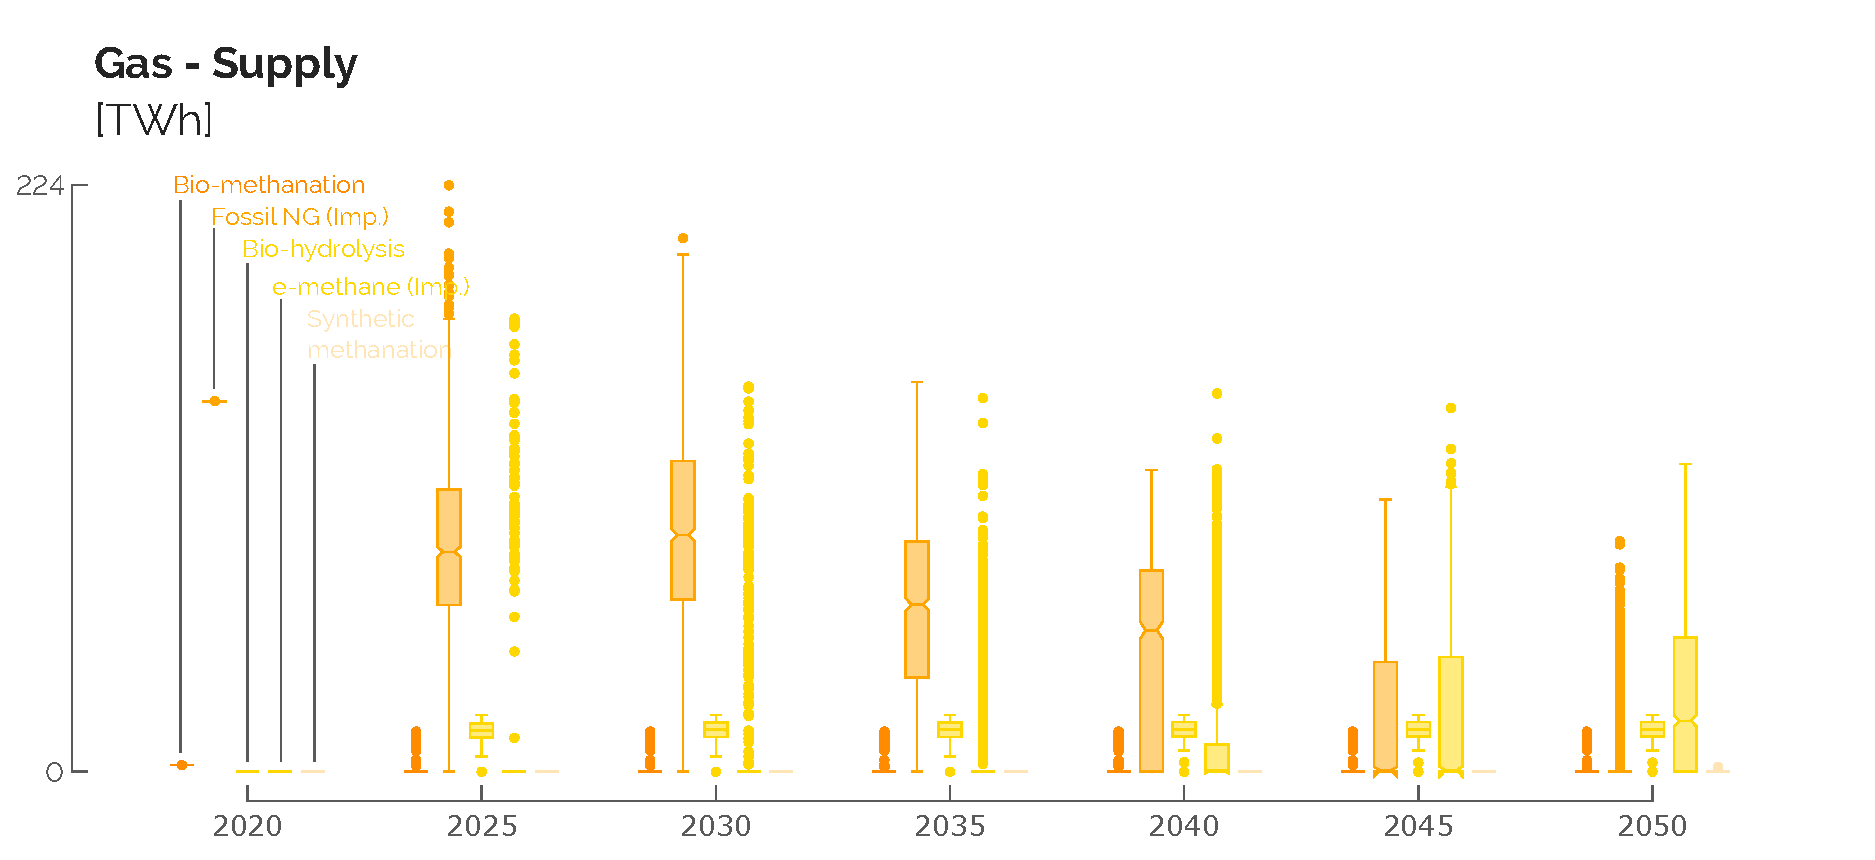
\includegraphics[width=\textwidth]{UQ_Gas_Prod.pdf}
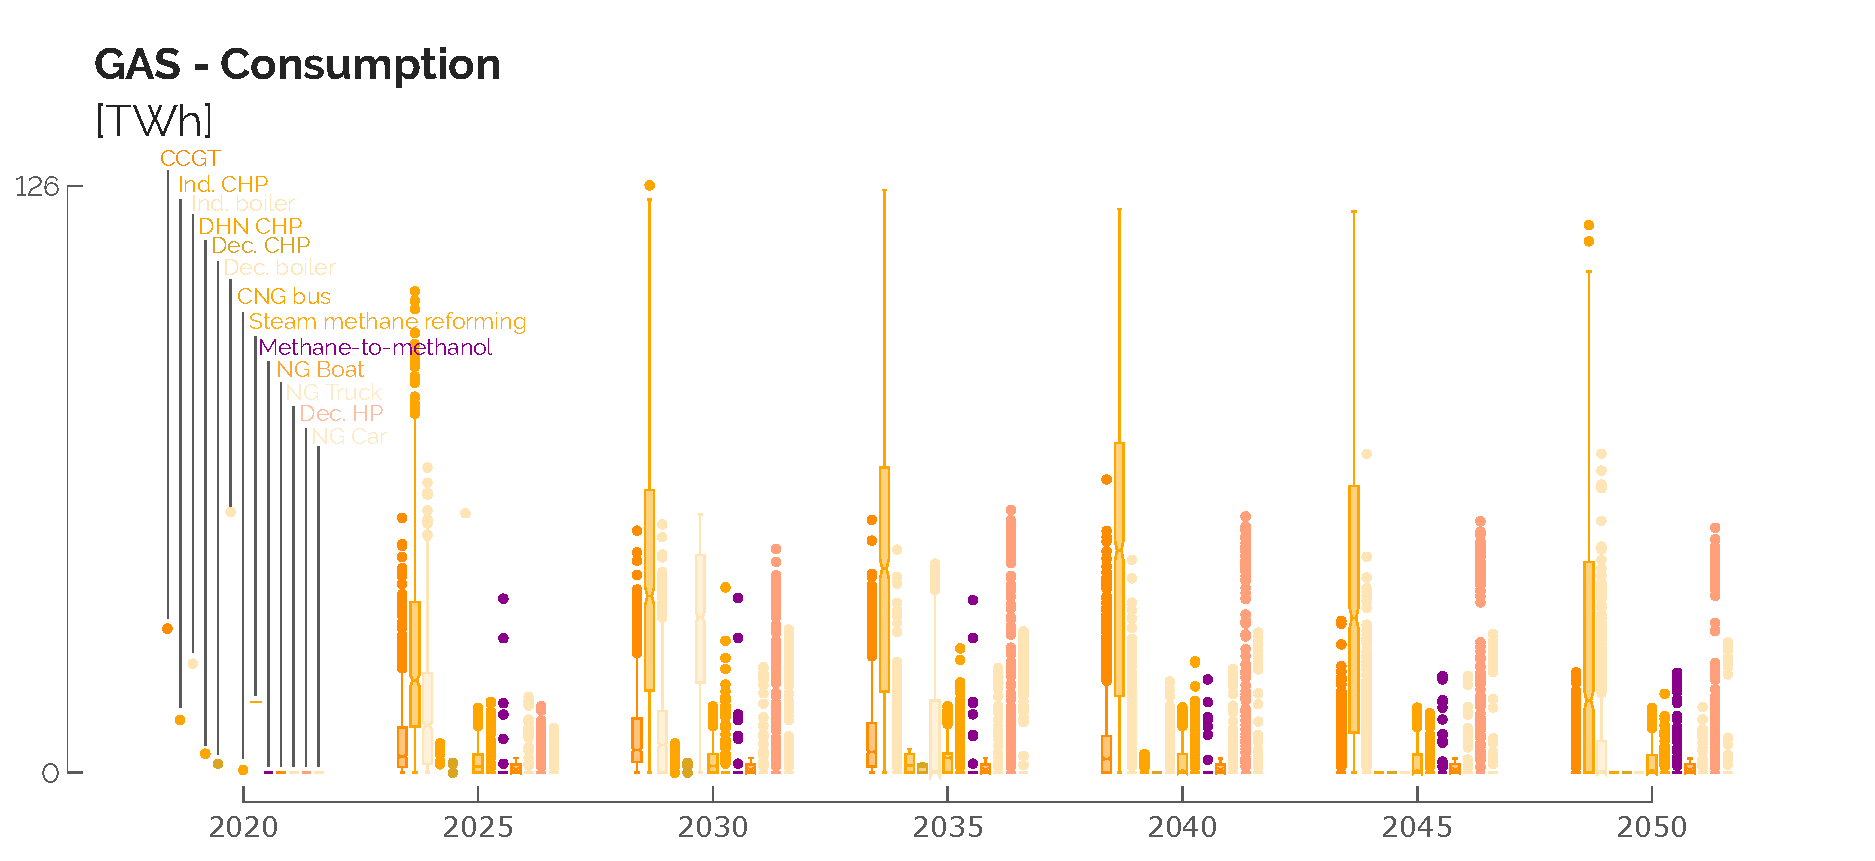
\includegraphics[width=\textwidth]{UQ_Gas_Cons.pdf}
\caption{Distribution of the different streams of supply (top) and consumption (bottom) of methane from the \acrfull{GSA}.}
\label{fig:results_uq_prod_cons_Gas}
\end{figure}

\begin{figure}[p!]
\centering
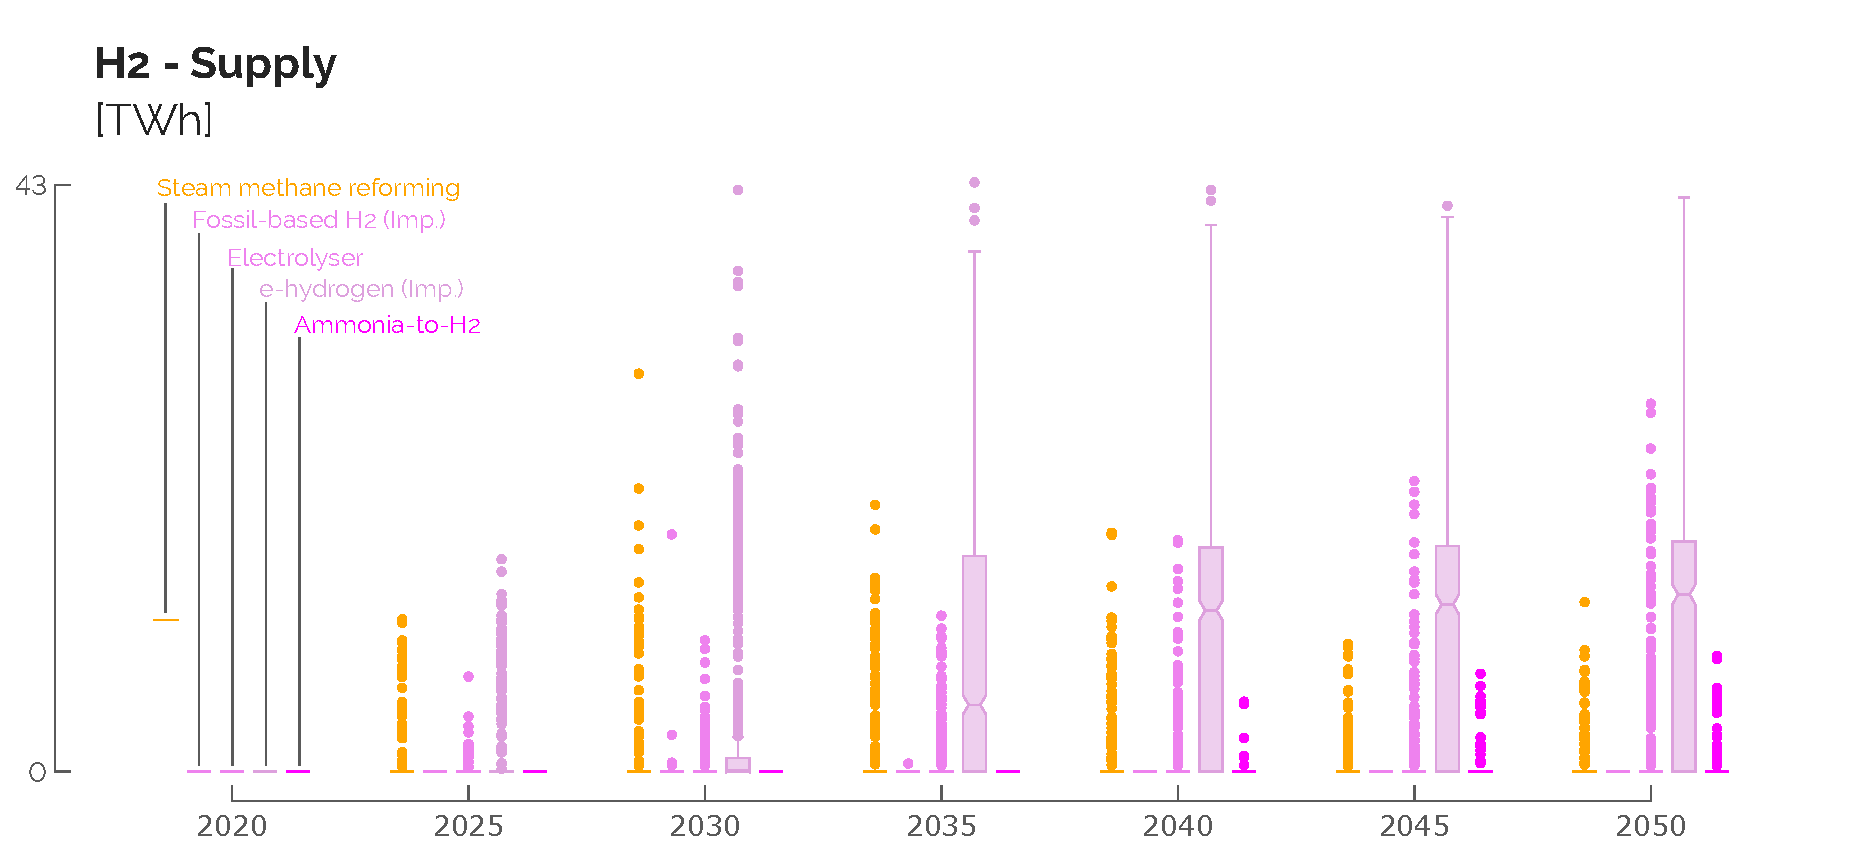
\includegraphics[width=\textwidth]{UQ_H2_Prod.pdf}
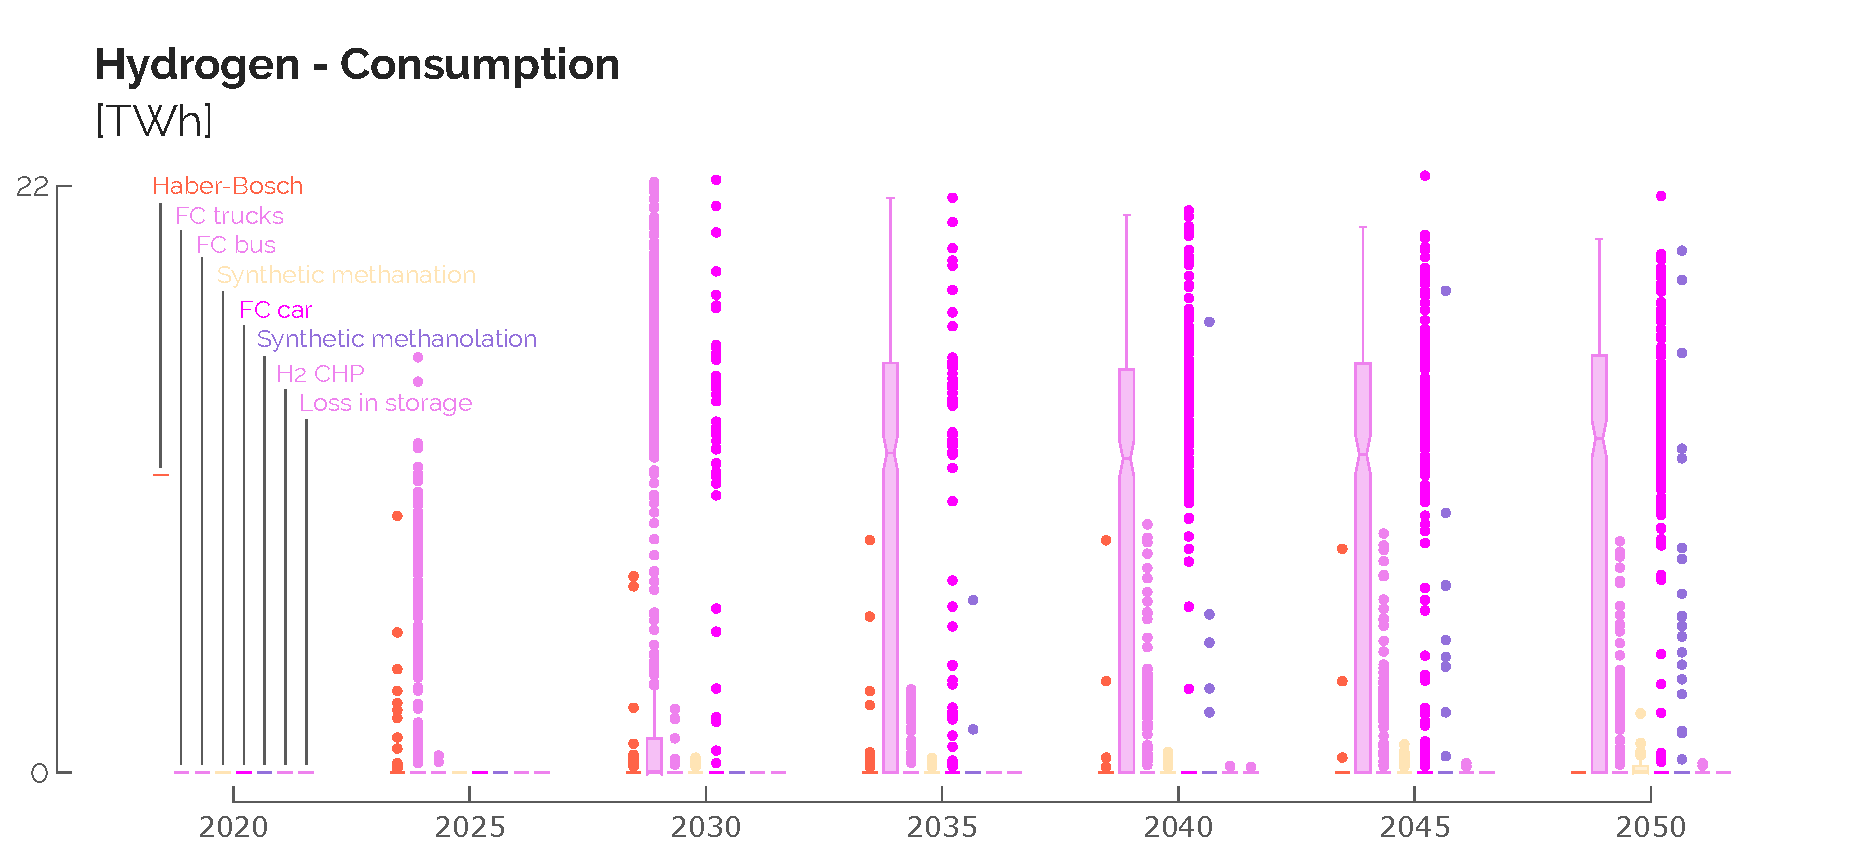
\includegraphics[width=\textwidth]{UQ_H2_Cons.pdf}
\caption{Distribution of the different streams of supply (top) and consumption (bottom) of hydrogen from the \acrfull{GSA}.}
\label{fig:results_uq_prod_cons_H2}
\end{figure}

\begin{figure}[p!]
\centering
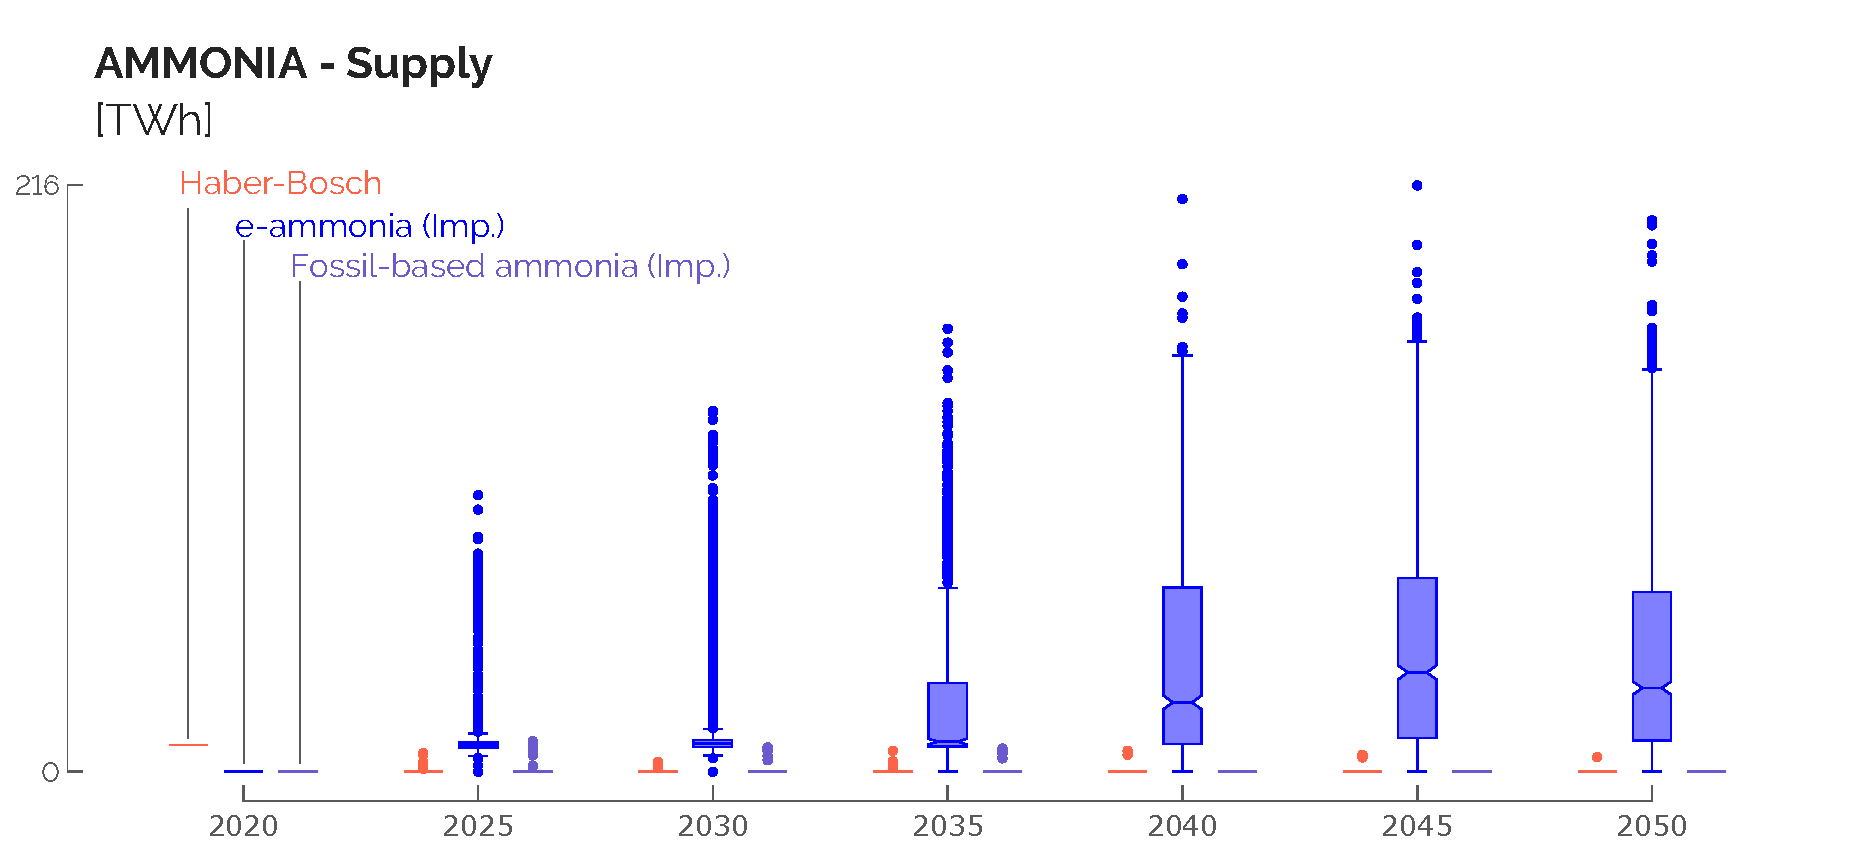
\includegraphics[width=\textwidth]{UQ_Ammonia_Prod.pdf}
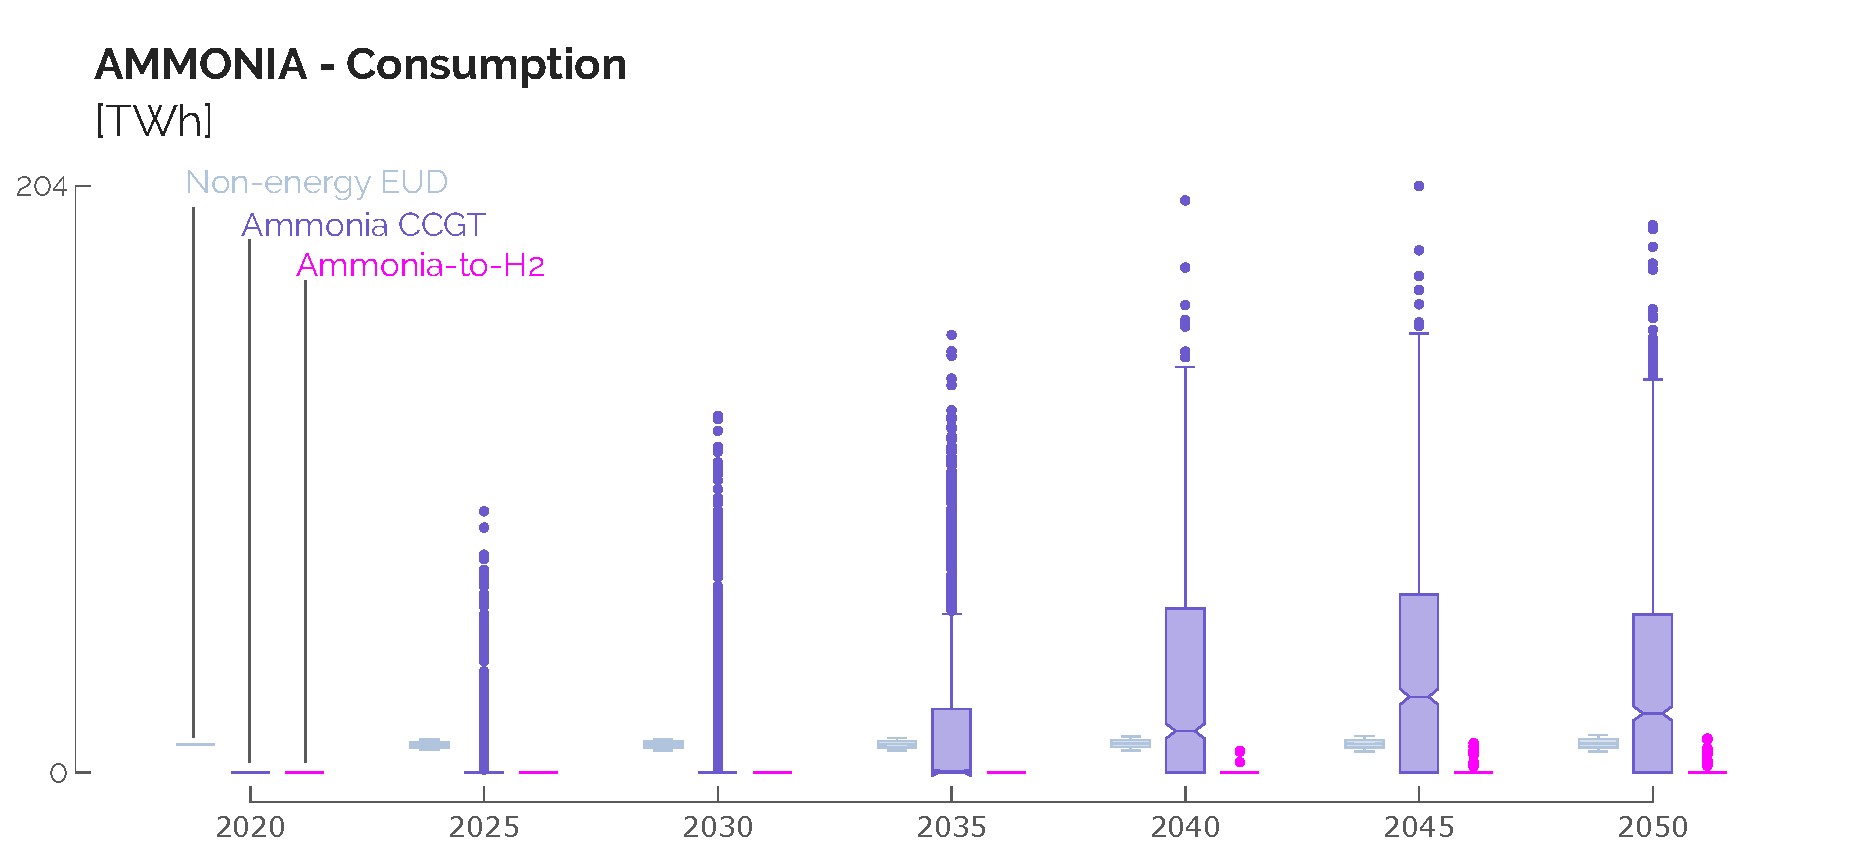
\includegraphics[width=\textwidth]{UQ_Ammonia_Cons.pdf}
\caption{Distribution of the different streams of supply (top) and consumption (bottom) of ammonia from the \acrfull{GSA}.}
\label{fig:results_uq_prod_cons_Ammonia}
\end{figure}

\begin{figure}[p!]
\centering
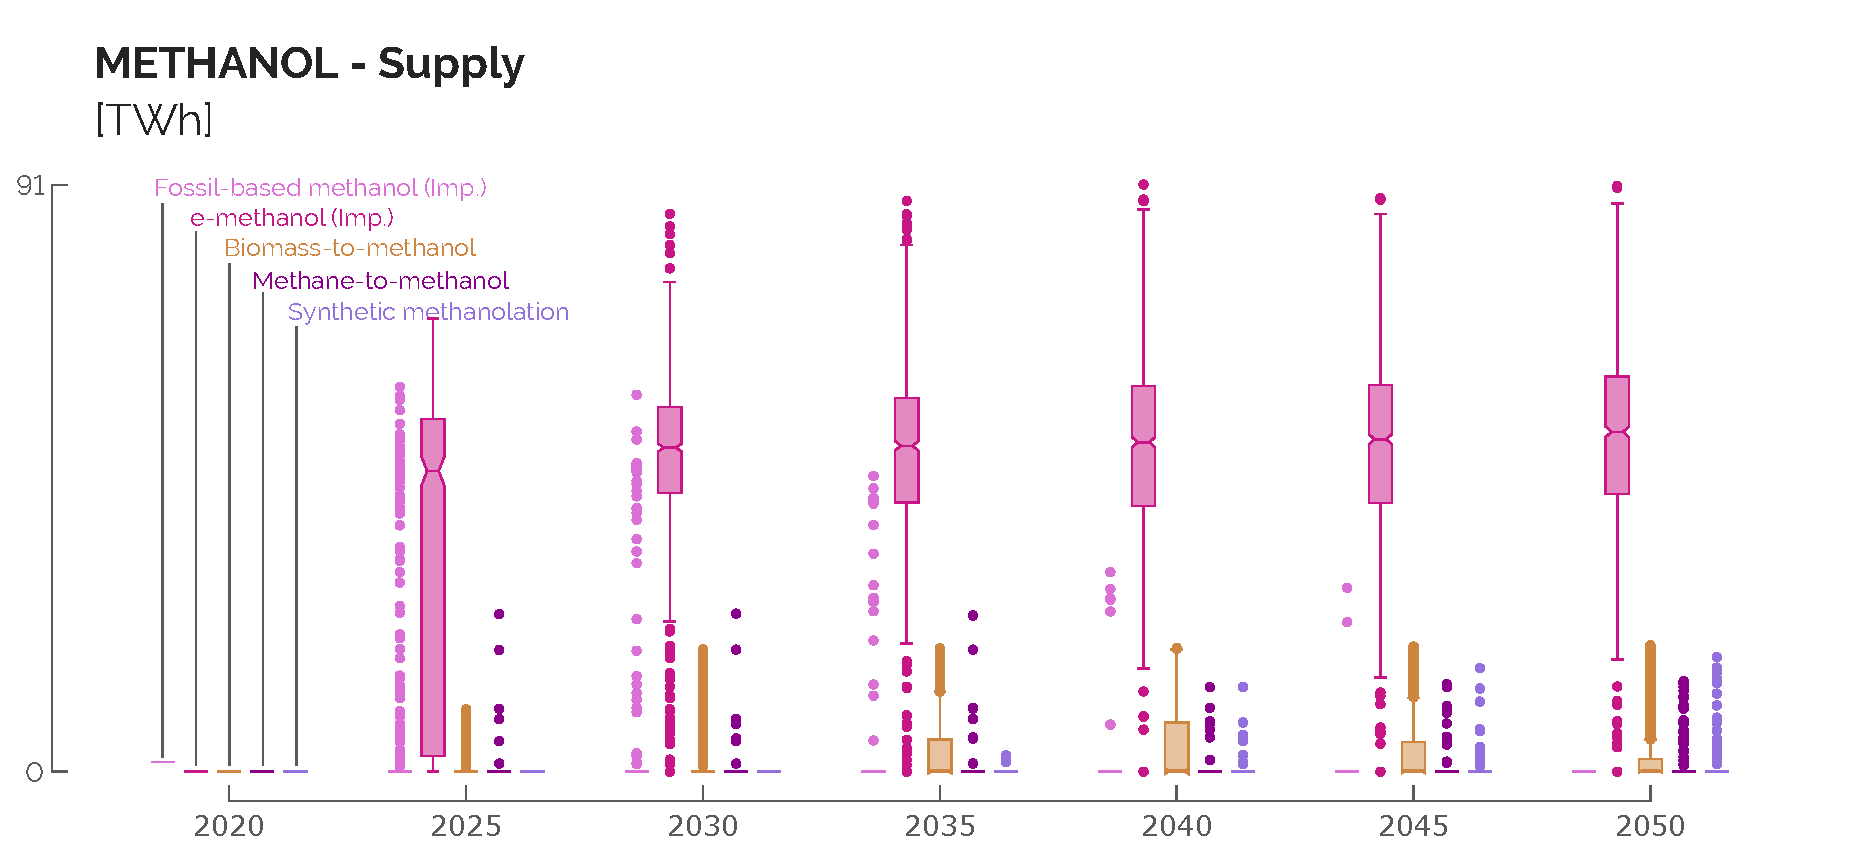
\includegraphics[width=\textwidth]{UQ_Methanol_Prod.pdf}
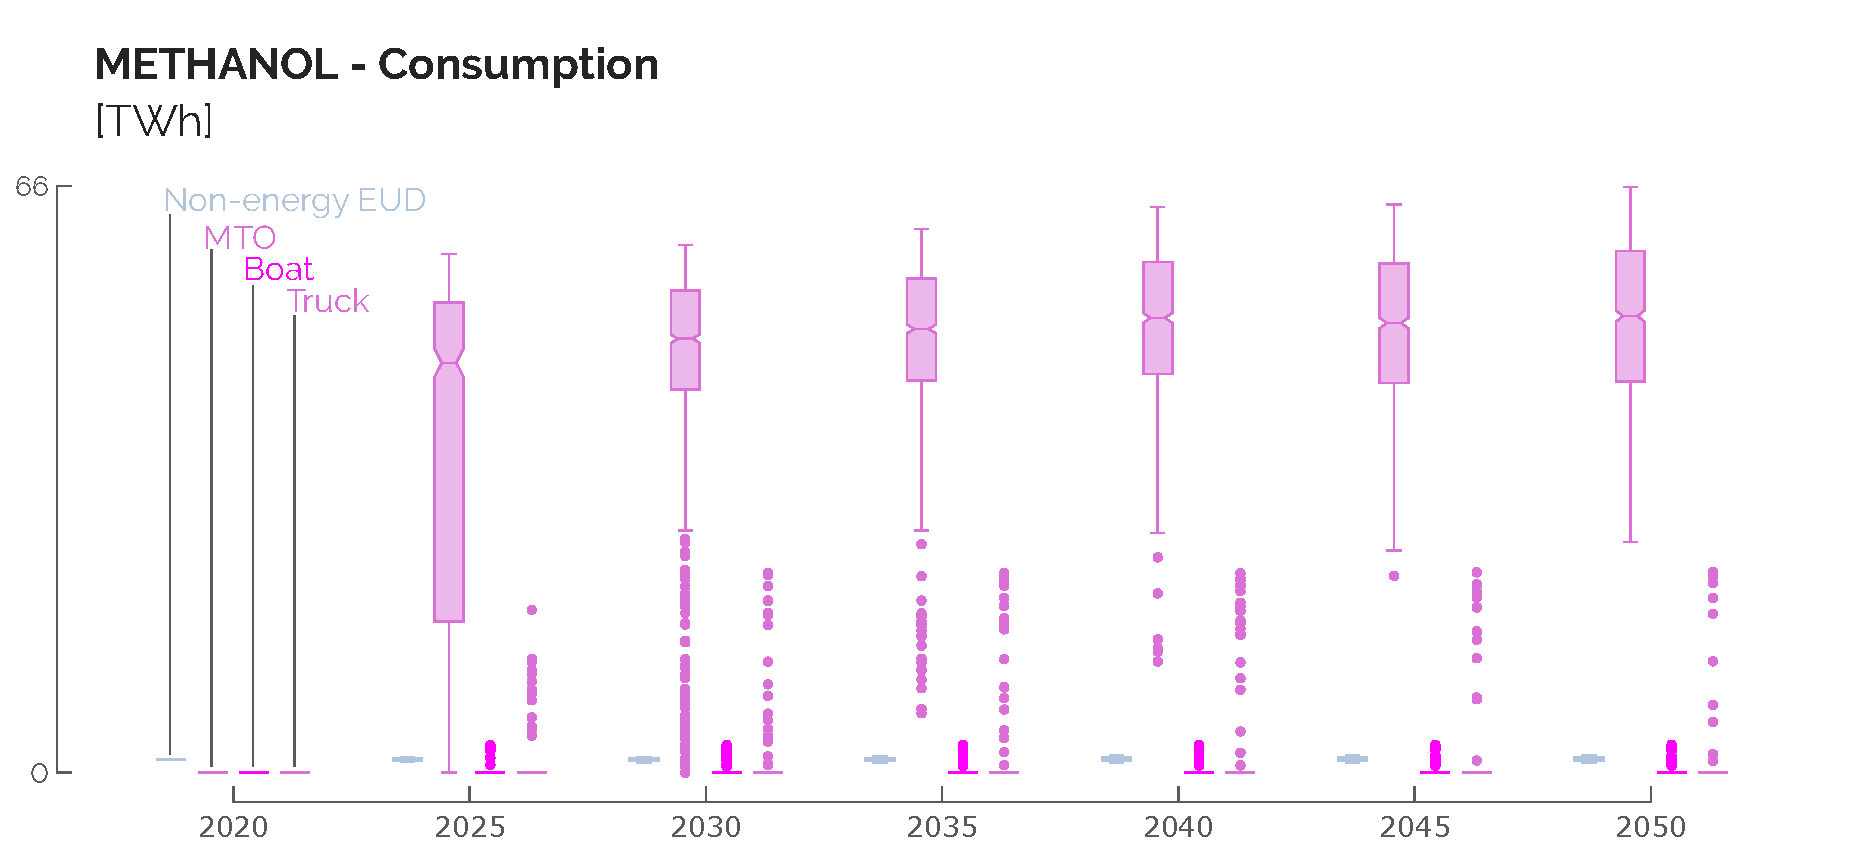
\includegraphics[width=\textwidth]{UQ_Methanol_Cons.pdf}
\caption{Distribution of the different streams of supply (top) and consumption (bottom) of methanol from the \acrfull{GSA}.}
\label{fig:results_uq_prod_cons_Methanol}
\end{figure}

\clearpage

\subsection{Installed capacities}
\label{app:UQ_tech_cap}


\begin{figure}[htbp!]
\centering
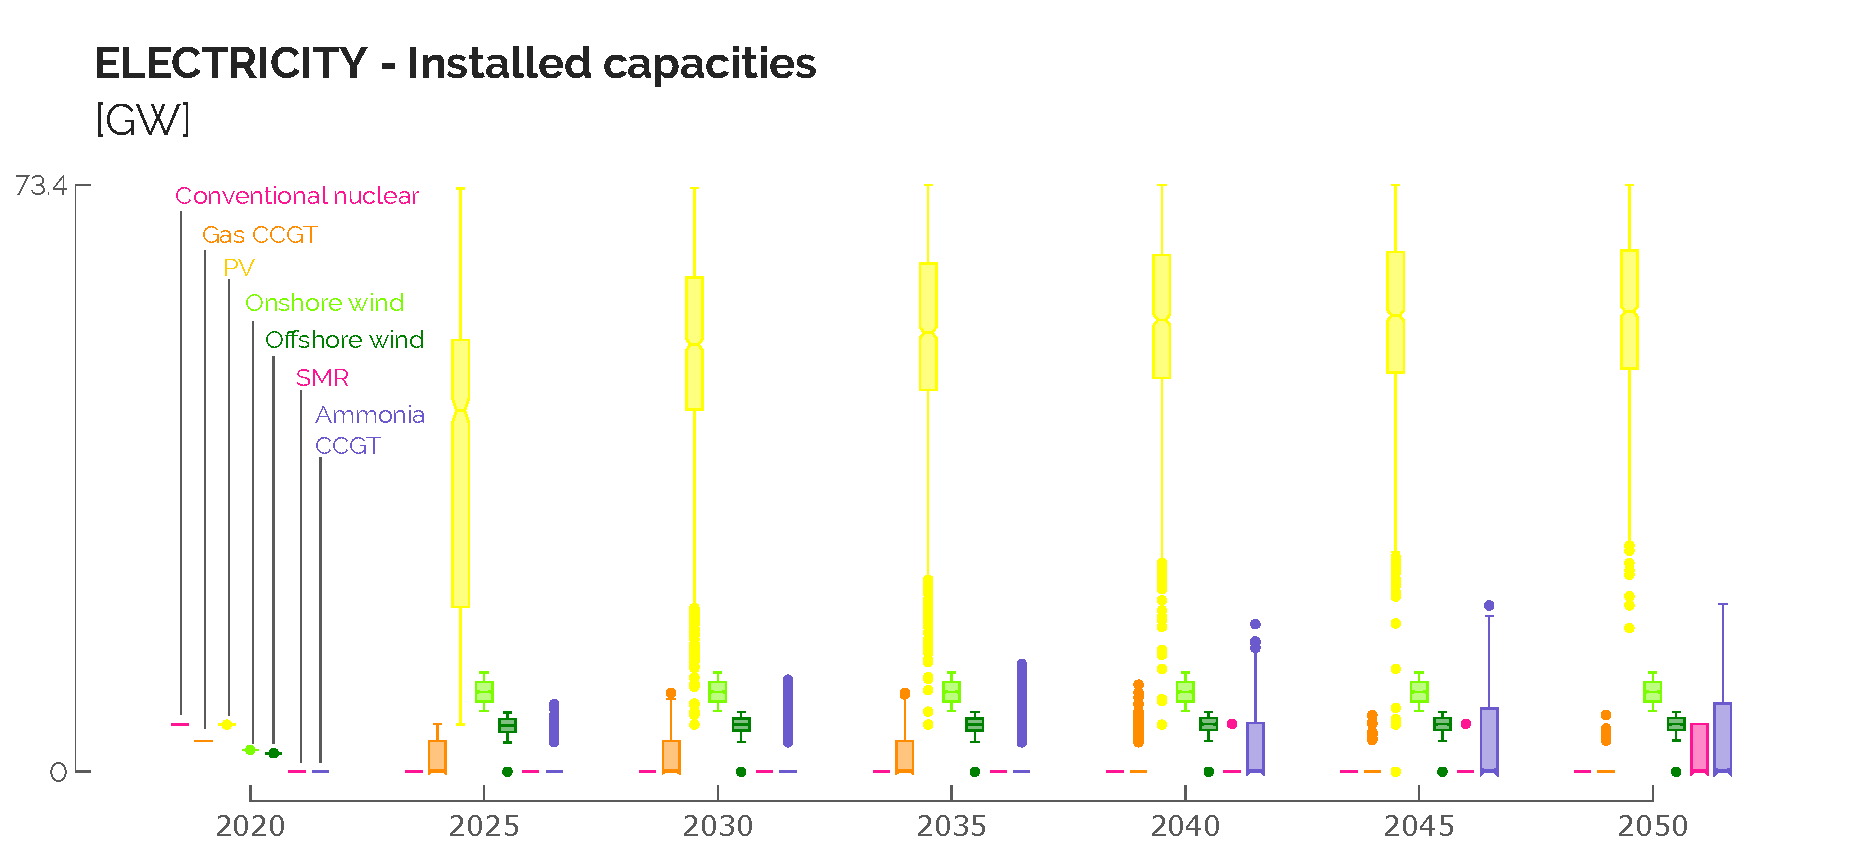
\includegraphics[width=0.9\textwidth]{ELECTRICITY_Tech.pdf}
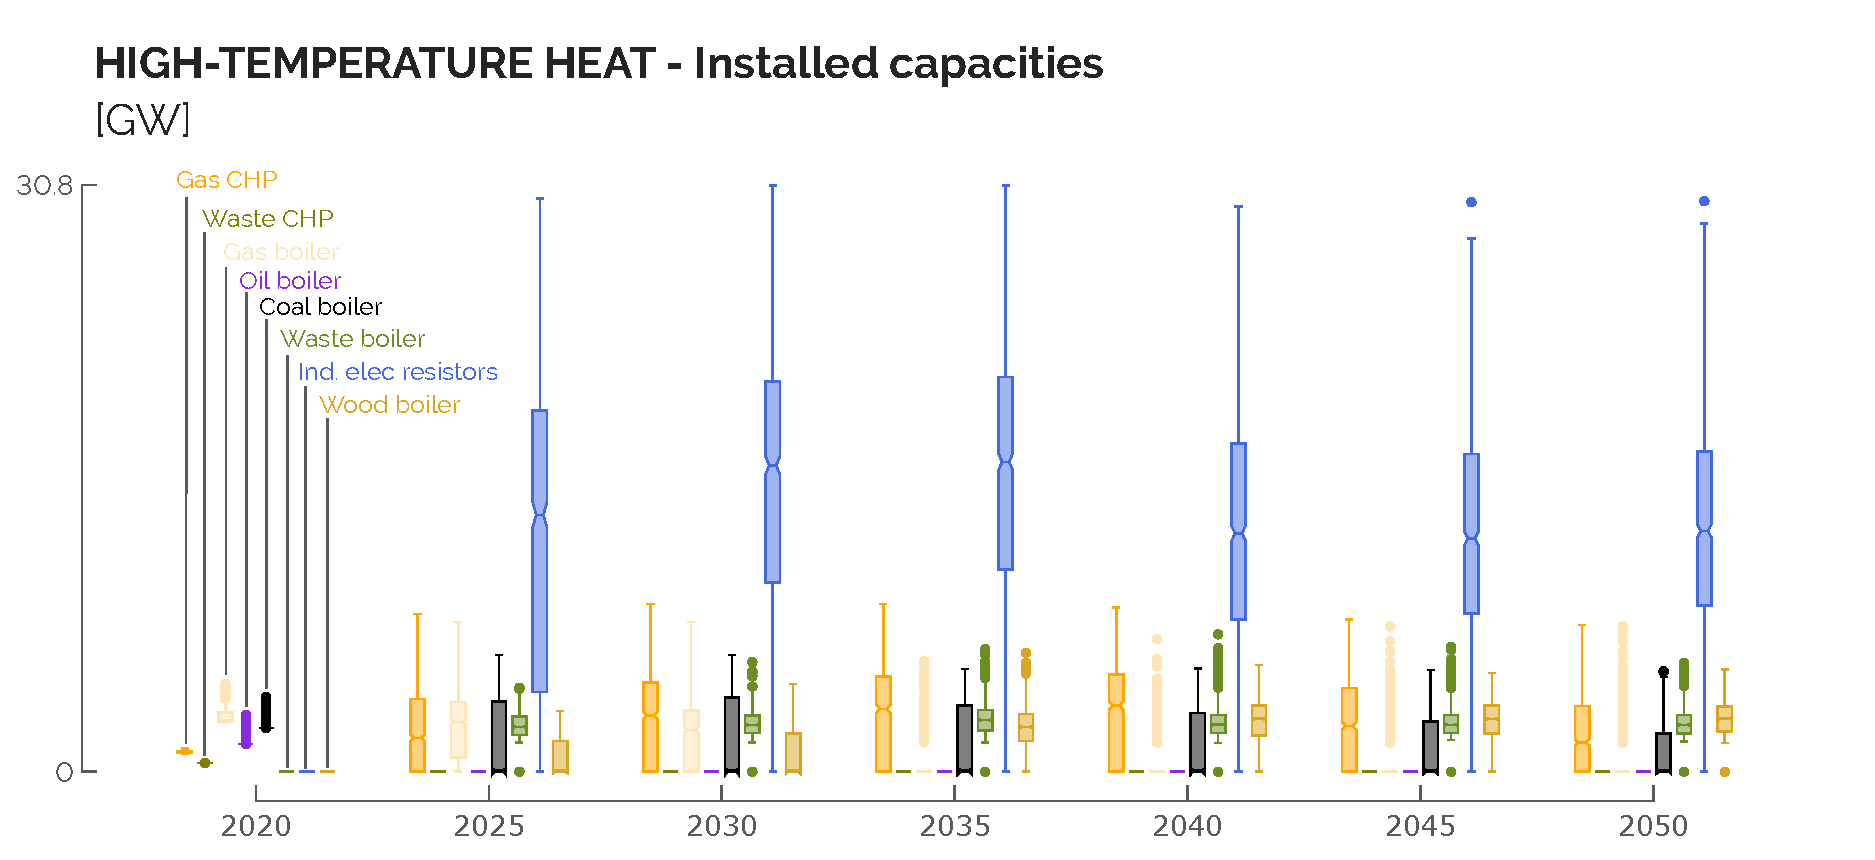
\includegraphics[width=0.9\textwidth]{HT_HEAT_Tech.pdf}
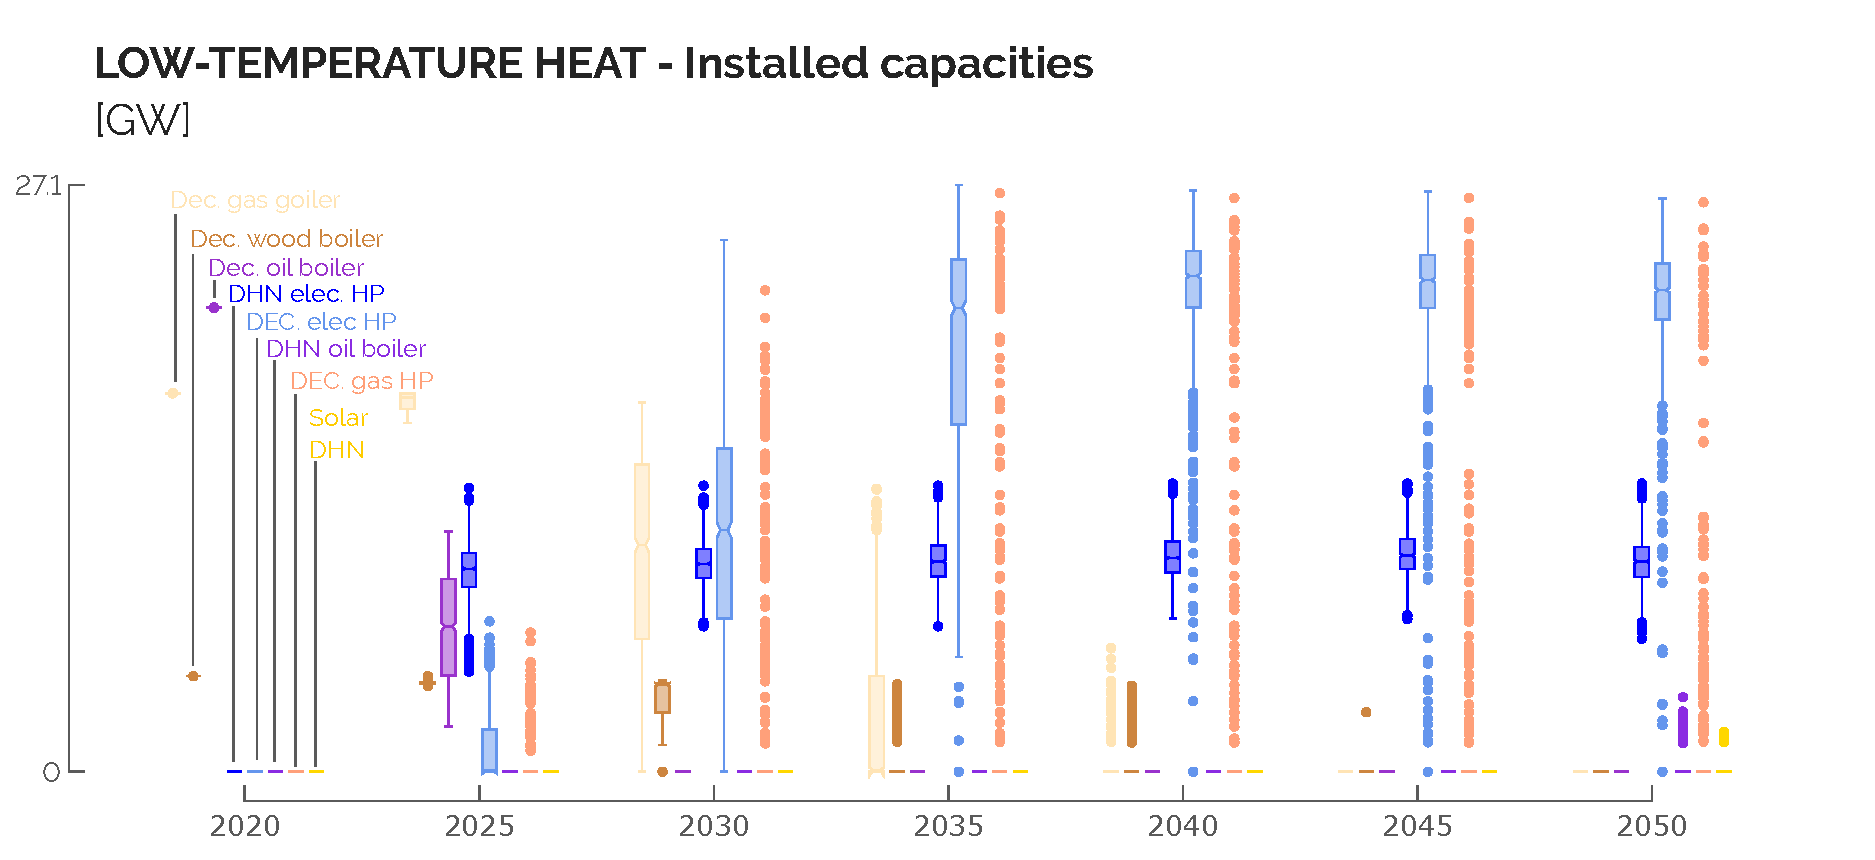
\includegraphics[width=0.9\textwidth]{LT_HEAT_Tech.pdf}
\caption{Distribution of the installed capacities among the end-use sectors of electricity, \gls{HT} and \gls{LT} heat from the \acrfull{GSA}.}
\label{fig:results_uq_tech_cap_ELEC_HT_LT}
\end{figure}

\begin{figure}[htbp!]
\centering
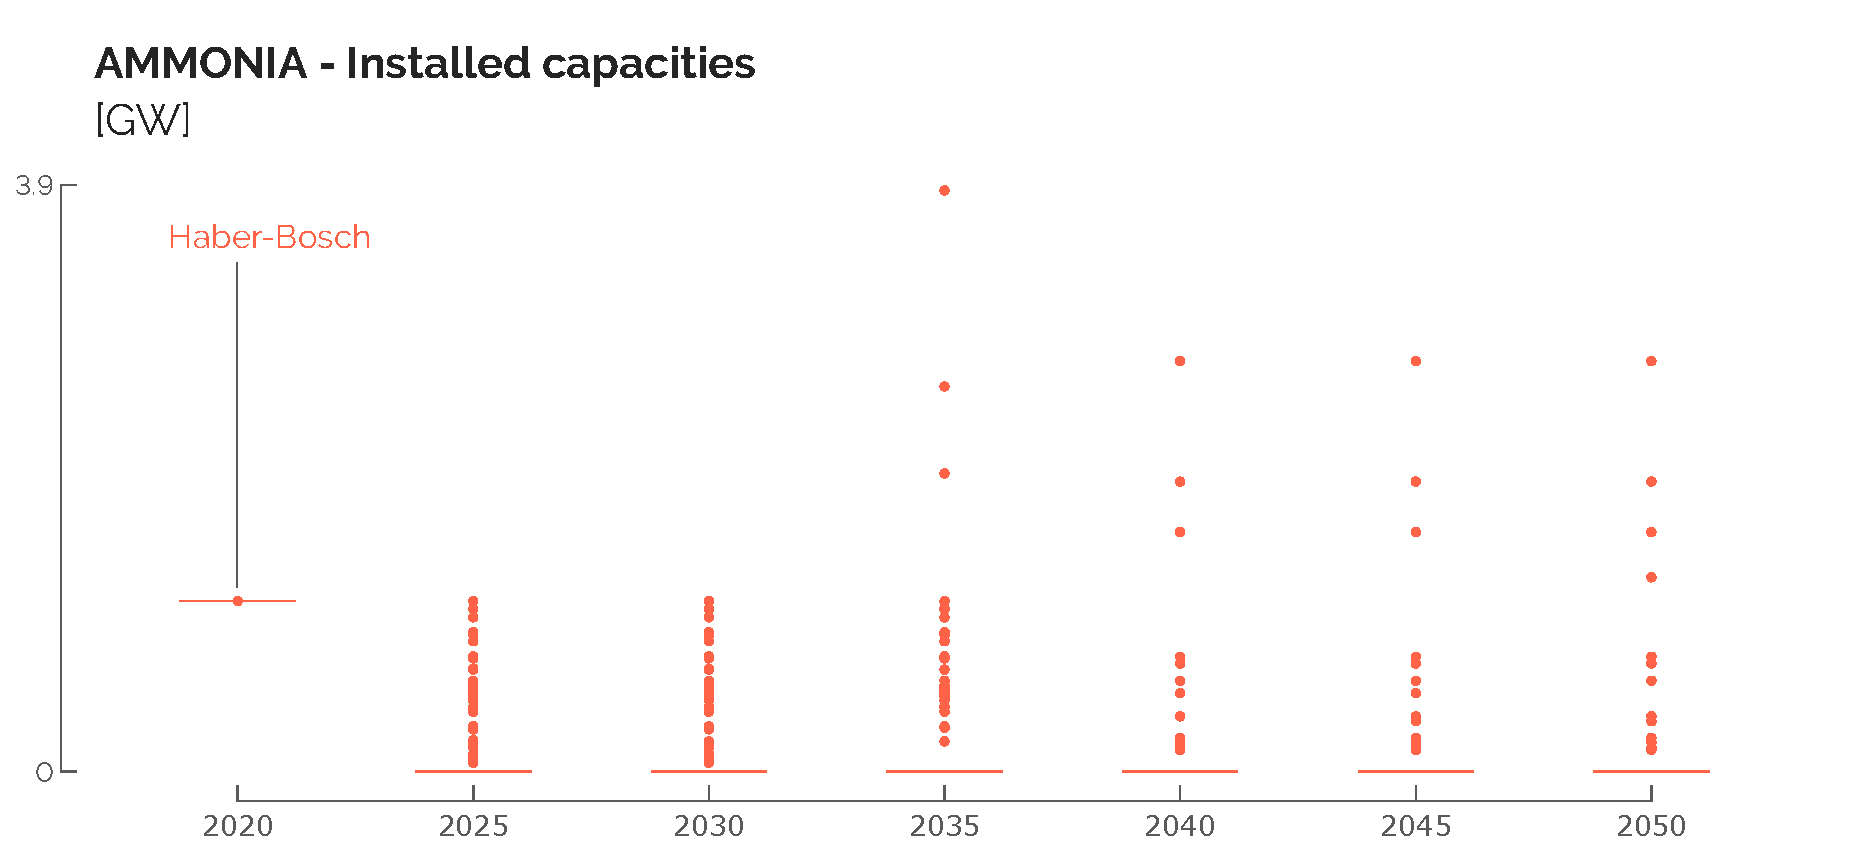
\includegraphics[width=\textwidth]{AMMONIA_Tech.pdf}
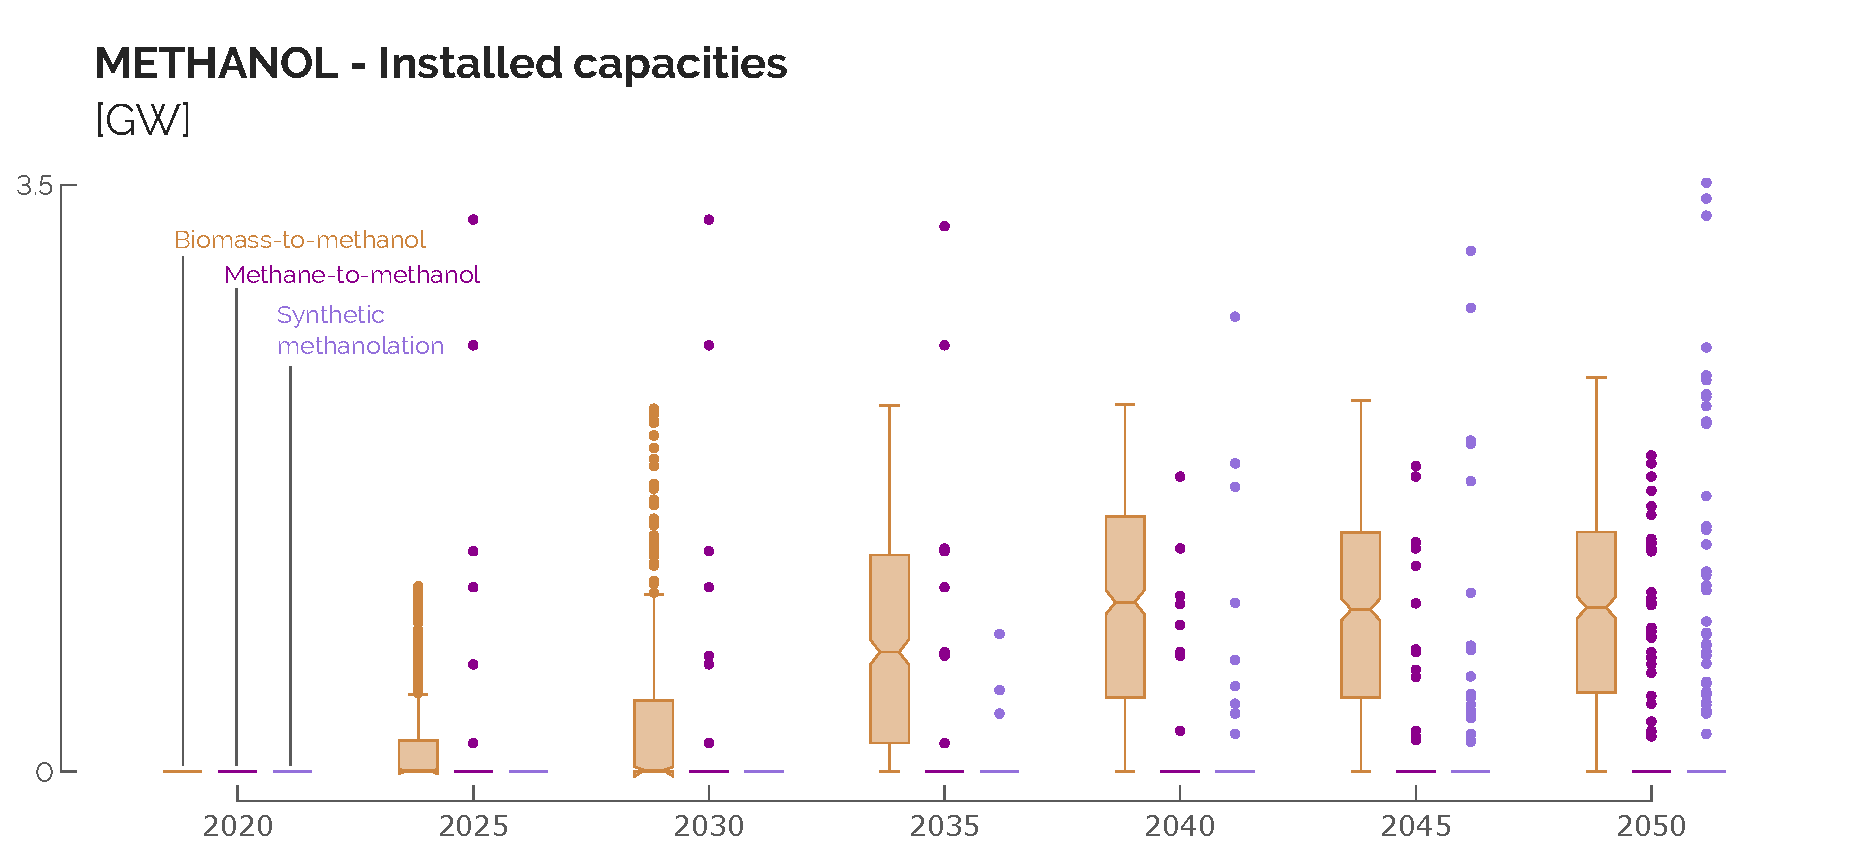
\includegraphics[width=\textwidth]{METHANOL_Tech.pdf}
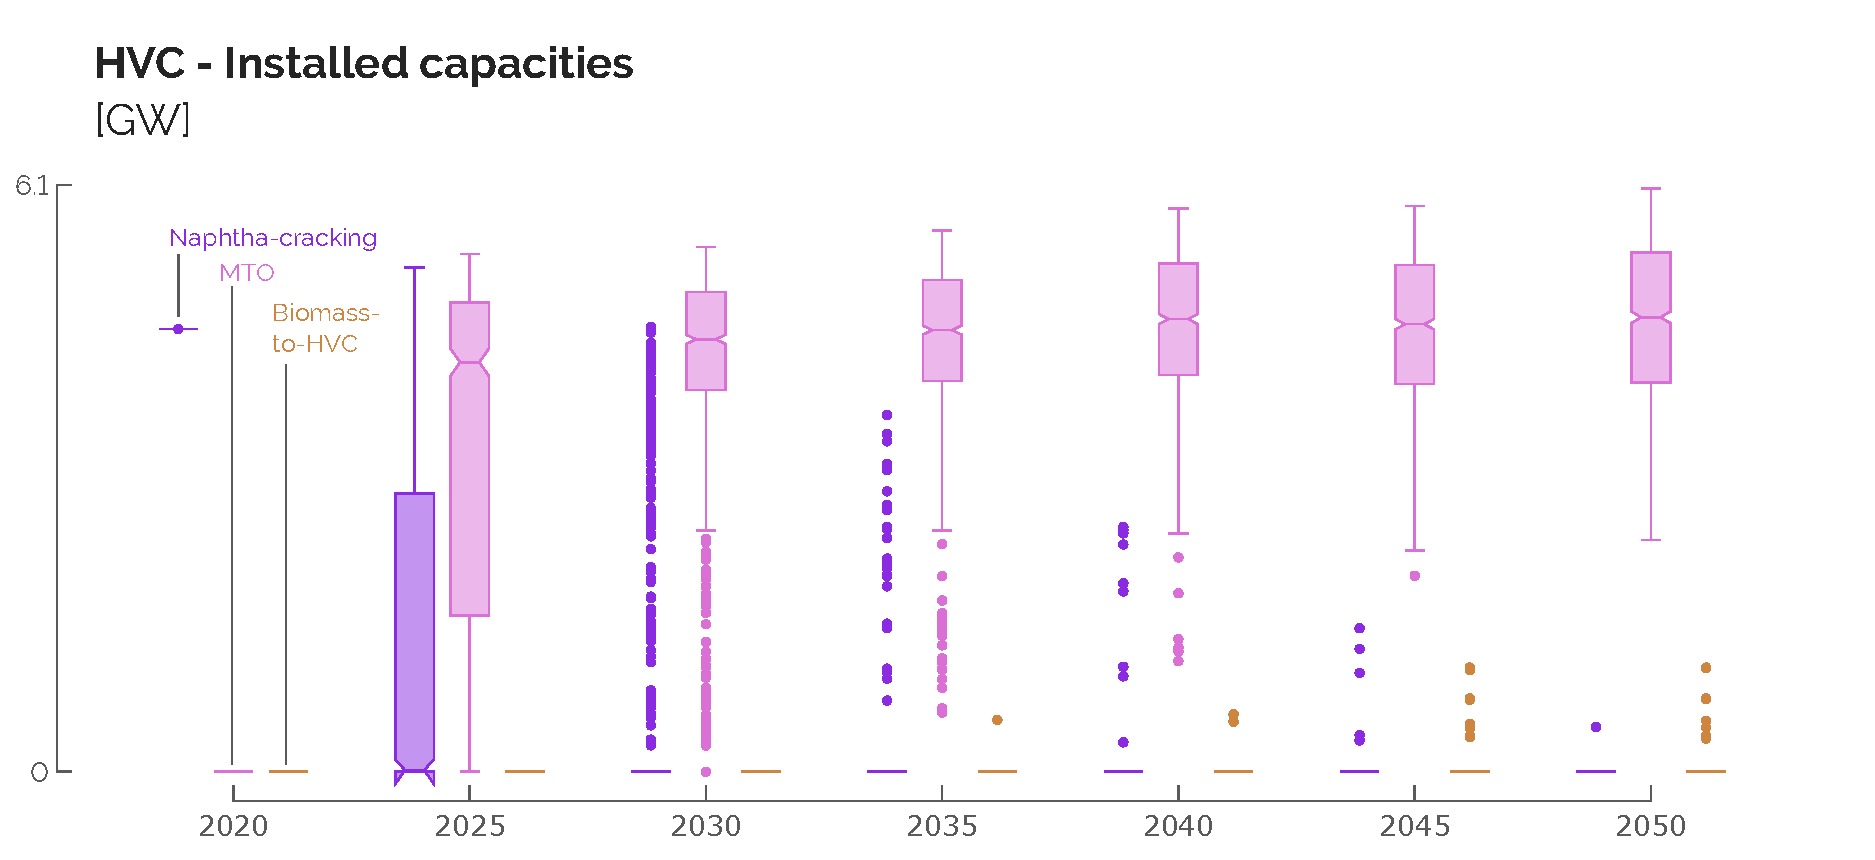
\includegraphics[width=\textwidth]{HVC_Tech.pdf}
\caption{Distribution of the installed capacities among the end-use sectors of ammonia, methanol and \gls{HVC} from the \acrfull{GSA}.}
\label{fig:results_uq_tech_cap_NED}
\end{figure}

\begin{figure}[htbp!]
\centering
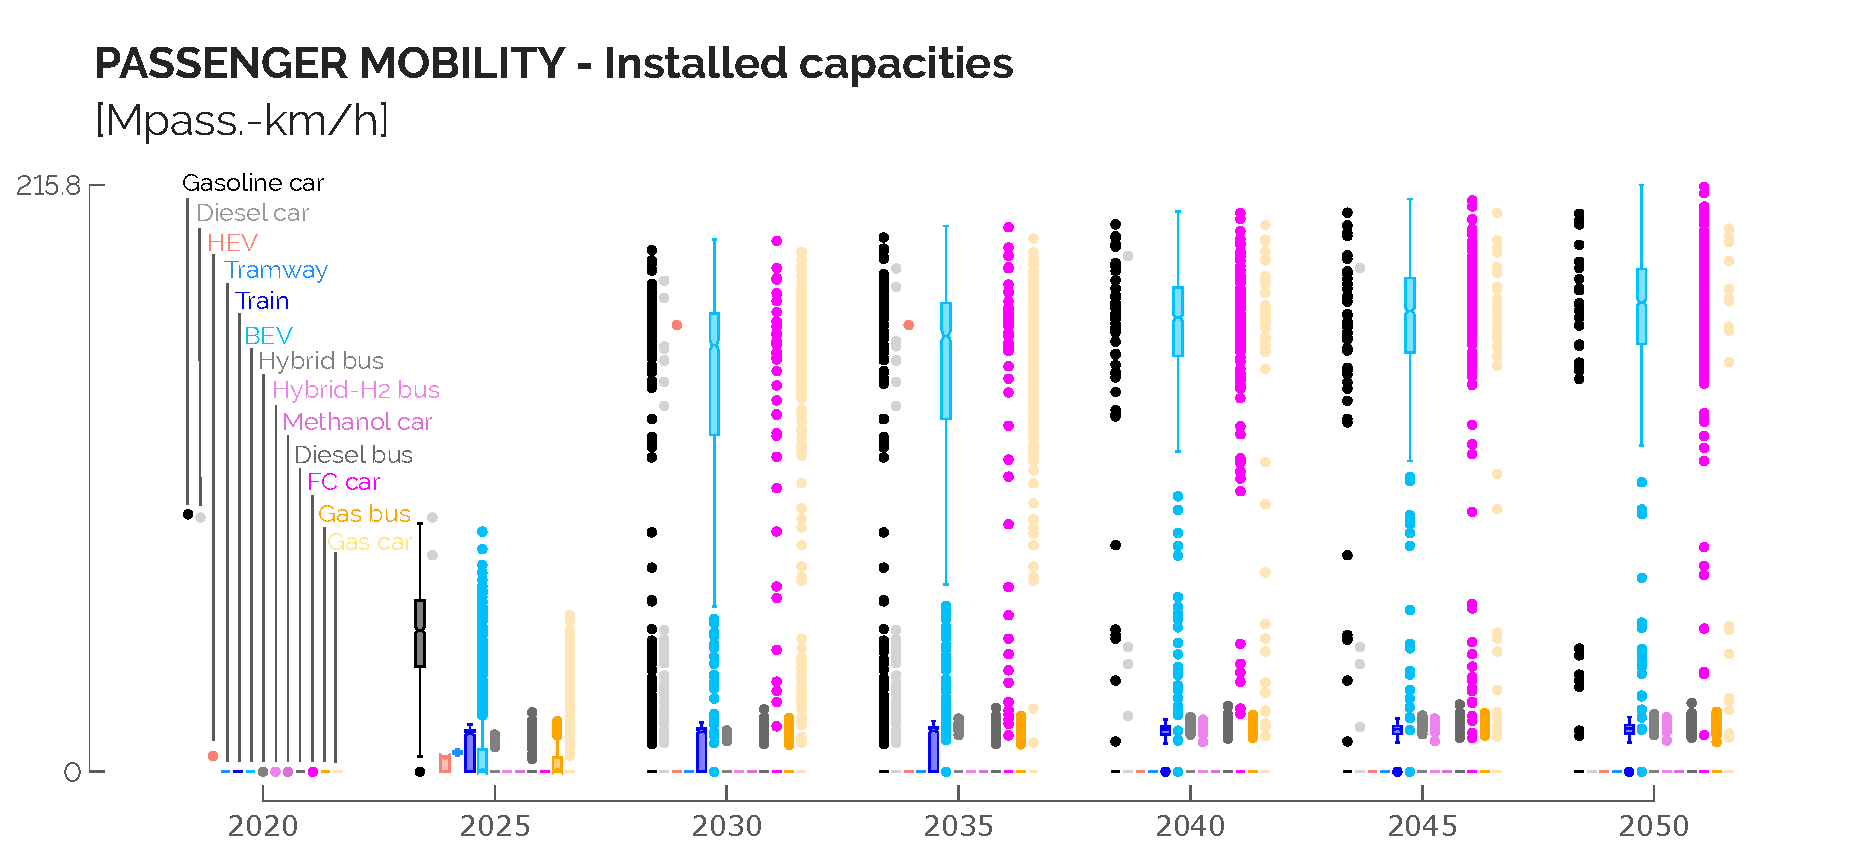
\includegraphics[width=\textwidth]{PASS_MOB_Tech.pdf}
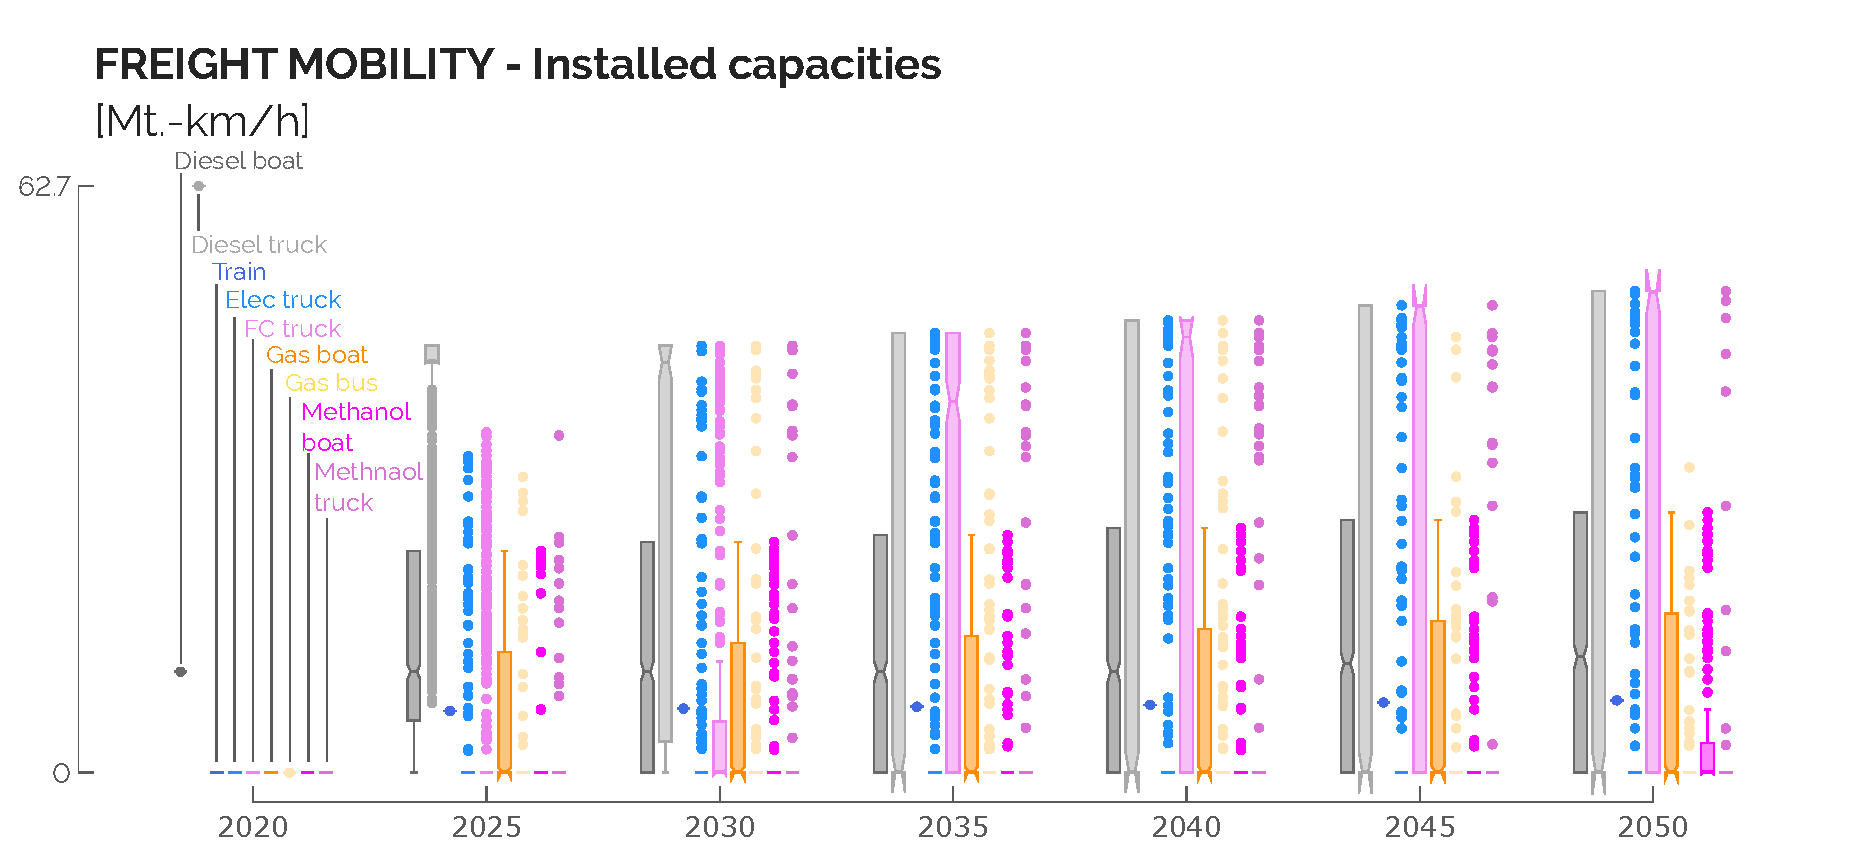
\includegraphics[width=\textwidth]{FREIGHT_MOB_Tech.pdf}
\caption{Distribution of the installed capacities among the end-use sectors of passenger and freight mobility from the \acrfull{GSA}.}
\label{fig:results_uq_tech_cap_MOB}
\end{figure}


\end{appendices}


\newpage

\section*{Acknowledgement}
Authors acknowledge the support of the Energy Transition Fund of Belgium.

%\section{References}
% If not using biblatex
% To set the bibliography style
%\bibliographystyle{unsrt} 
%\bibliography{bibliography/biblio}{}
% If using biblatex
\printbibliography[heading=bibintoc]
\end{document}
%%%%%%%%% End of the Report %%%%%%%%%